\ifnum \aluno=1
\renewcommand\chapterillustration{abertura-log.jpg}
\else
\renewcommand\chapterillustration{abertura-log-prof.jpg}
\fi
%Imagem da Wikimedia Commons - https://commons.wikimedia.org/wiki/File:Pedra_Azul_Milky_Way.jpg
\renewcommand\chapterwhat{Conceito de logaritmo.
Propriedades operacionais dos logaritmos. Função logarítmica.
Gráfico da função logarítmica  e sua relação com a função exponencial. Gráficos em escalas logarítmicas.}
\renewcommand\chapterbecause{Os logaritmos estão presentes em problemas de natureza exponencial sempre que a incógnita aparece no expoente. Esse tipo de questão é relevante em muitos problemas práticos como,  por exemplo, para calcular em quanto tempo uma dívida no cartão de crédito dobrará seu valor.

Os logaritmos também estão presentes em questões técnicas de muitas áreas do conhecimento, por exemplo na escala Richter, nas definições de decibel e de PH, no decaimento radioativo, na datação por carbono 14, na farmacologia e na homeopatia.

Os logaritmos são também úteis sempre que dados de magnitudes muito distintas estão representadas em um mesmo gráfico ou quando crescimentos relativos são mais importantes do que os valores absolutos. Gráficos nessa escala são muito utilizados para avaliar a evolução de ações da bolsa de valores e em processos que cresçam exponencialmente, como na pandemia de Covid-19.}





\chapter{Logaritmos e a Função Logarítmica}

\mbox{}\thispagestyle{empty}\newpage

\thispagestyle{empty}

\begin{center}
Projeto: LIVRO ABERTO DE MATEMÁTICA

\noindent \begin{tabular}{lcccr}

\includegraphics[scale=.15]{impa}& \quad\quad& 
\includegraphics[width=3cm]{logo} & \quad\quad& 
\includegraphics[scale=.24]{obmep} 
\end{tabular}
\end{center}

\vspace*{.3cm}

Cadastre-se como colaborador no site do projeto: \url{umlivroaberto.com}

Versão digital do capítulo:

\url{https://www.umlivroaberto.org/BookCloud/Volume_1/master/view/AF107.html}


\begin{tabular}{p{.15\textwidth}p{.7\textwidth}}
Título: & Logaritmos\\
\\
Ano/ Versão: & 2020 / versão 1.0 de 20 de agosto de 2020\\
\\
Editora & Instituto Nacional de Matem\'atica Pura e Aplicada (IMPA-OS)\\
\\
Realização:& Olimp\'iada Brasileira de Matem\'atica das Escolas P\'ublicas (OBMEP)\\
\\
Produção:& Livro Aberto\\
\\
Coordenação:& Fabio Simas e Augusto Teixeira (livroaberto@impa.br)\\
\\
  Autores: & Márcio Rostirolla Adames (UTFPR)\\
             & Rose Elizangela Martins Pedrosa (SEED - PR)\\
\\
Revisores: & Wanderley Rezende (UFF) \\ & Cydara Cavedon Ripoll (UFRGS) \\
                
\\
Design: & Andreza Moreira (Tangentes Design)\\
\\
  Ilustrações: & Márcio Rostirolla Adames \\ 
\\
Gráficos: & Beatriz Cabral e Tarso Caldas (Licenciandos da UNIRIO)\\
\\
  Capa: & (adaptado da) Foto "Pedra Azul Milky Way"\, de EduardoMSNeves, na Wikimedia Commons  \\

\end{tabular}
\vspace{.5cm}


\begin{minipage}[l]{5cm}
  
\includegraphics[width=3.5cm]{cc-by-nc-sa}
\end{minipage}\hfill
\begin{minipage}[r]{5cm}
{\Large  Patrocínio:}
  
  
\includegraphics[width=3.5cm]{itau}
\end{minipage}

\clearpage





\begin{apresentacao}
\section*{Contextualizando o ensino de logaritmos.}
A BNCC determina o estudo de logaritmos no ensino médio através das habilidades:

\begin{objetivos}{EM13MAT305}
Resolver e elaborar problemas com funções logarítmicas nos quais seja necessário compreender e interpretar a variação das grandezas envolvidas, em contextos como os de abalos sísmicos, pH, radioatividade, Matemática Financeira, entre outros.
\tcbsubtitle{EM13MAT403}
Analisar e estabelecer relações, com ou sem apoio de tecnologias digitais, entre as representações de funções exponencial e logarítmica expressas em tabelas e em plano cartesiano, para identificar as características fundamentais (domínio, imagem, crescimento) de cada função.
\end{objetivos}

Os logaritmos estão presentes em problemas de natureza exponencial sempre que a incógnita aparece no expoente. O logaritmo é o expoente ao qual a base deve ser elevada para obter-se determinado número\notarodape{Chamado de logaritmando.}. Estamos convencidos que esse entendimento conceitual é importante para a interpretação de situações em diversos contextos e subsequente construção de modelos, análise de resultados, comunicação desses resultados e  tomadas de decisão, etapas essas previstas nas competências 1, 2, 3 e 4 da BNCC.


Alguns contextos frequentemente ligados aos logaritmos são os juros compostos da matemática financeira, a escala Richter, as definições de decibel e de PH. Eles também estão presentes no decaimento radioativo, na datação por carbono 14, na farmacologia e na homeopatia.

Além dos contextos específicos, os logaritmos são um recurso para representarmos dados de magnitudes muito distintas em um mesmo gráfico, como no caso da pandemia de Covid19, e quando os crescimentos relativos são mais importantes que os valores propriamente ditos, como no caso de ações da bolsa de valores.

Devido aos muitos contextos envolvidos, o conteúdo também é uma oportunidade para auxiliar no desenvolvimento de outras habilidades da BNCC:
\begin{itemize}
\item O logaritmo é uma ferramenta natural para problemas de matemática financeira quando a incógnita é o tempo necessário para chegar a determinado objetivo, o que está relacionado à habilidade:
\end{itemize}

\begin{objetivos}{EM13MAT303}
Interpretar e comparar situações que envolvam juros simples com as que envolvem juros compostos, por meio de representações gráficas ou de análise de planilhas, destacando o crescimento linear ou exponencial de cada caso.
\end{objetivos}

\begin{itemize}
\item Situações envolvendo juros compostos são comuns no cotidiano familiar. Saber como isso funciona pode auxiliar na tomada de decisão, por exemplo, para fazer uma aplicação ou saldar uma dívida.
\end{itemize}

\begin{objetivos}{EM13MAT203}
Aplicar conceitos matemáticos no planejamento, na execução e na análise de ações envolvendo a utilização de aplicativos e a criação de planilhas (para o controle de orçamento familiar, simuladores de cálculos de juros simples e compostos, entre outros), para tomar decisões.
\end{objetivos}

\begin{itemize}
\item Dados relacionados a diferentes aspectos da natureza, podem ser apresentados por meio de gráficos em escala logarítmica, sendo o conhecimento desse conteúdo necessário na apresentação dos dados e na análise dos mesmos.
\end{itemize}

\begin{objetivos}{EM13MAT101}
Interpretar criticamente situações econômicas, sociais e fatos relativos às Ciências da Natureza que envolvam a variação de grandezas, pela análise dos gráficos das funções representadas e das taxas de variação, com ou sem apoio de tecnologias digitais.
\end{objetivos}

\begin{objetivos}{EM13MAT104}
Interpretar taxas e índices de natureza socioeconômica (índice de desenvolvimento humano, taxas de inflação, entre outros), investigando os processos de cálculo desses números, para analisar criticamente a realidade e produzir argumentos.
\tcbsubtitle{EM13MAT102} Analisar tabelas, gráficos e amostras de pesquisas estatísticas apresentadas em relatórios divulgados por diferentes meios de comunicação, identificando, quando for o caso, inadequações que possam induzir a erros de interpretação, como escalas e amostras não apropriadas.
\end{objetivos}



\section*{O que dizem as pesquisas sobre o tema?}

As quatro competências 1, 2, 3 e 4 da BNCC \cite{BNCC2018} \notarodape{de um total de cinco} indicam um foco em problemas concretos e aplicabilidade na vida real. 

Também destacam a importância das questões praticas, os testes utilizados para avaliar o desempenho dos estudantes em larga escala (de sistemas educacionais inteiros, como o SAEB e o PISA). Por exemplo, em \cite[p.139]{OCDE2016}:

\textit{"Isto é, o PISA analisa até que ponto estudantes dessa idade sabem lidar adequadamente com a matemática ao serem confrontados com certos problemas e situações, a maioria apresentada em contextos do mundo real."}


Ressaltamos aqui que a preocupação com questões do mundo real está presente, em maior ou menor grau, nos livros didáticos aprovados pelo PNLD, contudo esses livros usualmente acrescentam as aplicações em cima de uma abordagem tradicional. As pesquisas sobre o tema parecem apontar que algumas dificuldades encontradas pelos estudantes podem estar relacionadas a essa forma de trabalhar o conteúdo.

%%%%%%%%%%%%%%%%%%%%%%%%%%%%%%%%


	Muitos trabalhos buscam entender, especificamente, as dificuldades no estudo de logaritmos.
	 
	Um dos trabalhos encontrados \cite{Liang2005} estudou estatisticamente o desempenho dos estudantes em questões propondo avaliar o desempenho nas categorias computação, entendimento e aplicação \notarodape{aplicadas na matemática e não em questões da vida real}, baseado-se em uma taxonomia de Bloom modificada, e concluiu que os estudantes têm maior dificuldade nas questões de entendimento e de aplicação. A análise deles é que parecem haver erros devido ao não entendimento conceitual do conteúdo, apesar da razoável capacidade operacional.

Na dissertação \cite{Berezovski2004}, a autora buscou analisar e descrever as principais causas de problema no entendimento dos estudantes ao aprender logaritmos e chegou à conclusão que vários estudantes tiveram dificuldades em entender os logaritmos como números e em reconhecer as propriedades dos logaritmos. Ela destacas duas causas possíveis para essas dificuldades:
	\begin{itemize}
	\item obstáculos cognitivo-epistemológicos na compreensão dos logaritmos como números e suas propriedades operatórias;
	\item o material didático, que pode estar focado demasiadamente nos conceitos de exponenciação e de função exponencial (tratando logaritmo como conceito secundário).
	\end{itemize}

No trabalho \cite{Kenney2013}, os autores discutem dificuldades que perceberam nos estudantes ao buscar entender o conteúdo de logaritmos. As dificuldades relatadas são:
	\begin{itemize}
	\item perceber o logaritmo como uma função (que pode ter origem em dificuldades com os conceitos de função exponencial ou função inversa);
	\item entender a notação corretamente; 
	\item entender e aplicar as propriedades dos logaritmos.
	\end{itemize}
Eles relatam, ainda, que outros autores também perceberam dificuldades semelhantes em seus trabalhos.

No trabalho \cite{Panagiotou2011}, o autor considera o uso da história no ensino de matemática e faz uma proposta concreta para o conteúdo de logaritmos. O autor afirma que a introduzir os logaritmos pela definição de Euler pode tornar difícil a compreensão do conceito de logaritmo e posa vários questionamentos difíceis de responder a partir desse ponto de vista.

No trabalho \cite{Weber2016}, o autor (Weber) explora detalhadamente a causa das dificuldades e conclui que os erros no entendimento dos logaritmos podem ser causados pela introdução do tema como a inversa de uma exponencial, pois os alunos não podem aplicá-lo diretamente. Ele apresenta os seguintes argumentos para isso:
\begin{itemize}
\item a definição de Euler\notarodape{Que define a função logarítmica como a inversa da função exponencial.} surgiu posteriormente ao surgimento dos logaritmos e reflete a visão de um especialista com grande experiência\notarodape{... e não de alguém entrando em contato com o assunto};
\item definições indiretas (a de Euler e outras) são pouco operacionais (não permitem o cálculo do logaritmo diretamente);
\item há similaridades no ensino de logaritmos com o ensino de divisão (inversa à multiplicação), mas a divisão é ensinada através de diversos contextos, ao contrário da elegância lógica dos logaritmos.
\end{itemize}
	
Assim os estudos parecem indicar que há espaço para a melhoria dos resultados no ensino-aprendizagem de logaritmos por meio de uma metodologia focada na introdução dos conceitos através das aplicações e não no conteúdo matemático formal.

Uma das possibilidades encontradas foi a de introduzir o conteúdo baseado no desenvolvimento histórico do conceito por Napier e Briggs (por exemplo em \cite{Pedrosa2018} e \cite{Panagiotou2011}), o que pode ser bastante interessante, mas não tem o foco na resolução de problemas práticos recomendada pela BNCC e pelos testes de larga escala.

Outra possibilidade encontrada foi a da Educação Matemática Realística (EMR), que busca engajar os estudantes através de contextos significativos e, ao invés de apresentar os conteúdos formais plenamente desenvolvidos, permite aos estudantes realizarem seus próprios raciocínios informais e formalizarem seus raciocínios progressivamente, indo do concreto para o abstrato.

De acordo com  \cite{HeuvelPanhuizen}, a Educação Matemática Realística (EMR) é uma teoria de instrução específica para matemática, que foi desenvolvida na Holanda. A principal característica da EMR é o uso de situações \textit{realistas}; que tem uma posição de destaque no processo de aprendizagem. Estas situações servem como fonte para iniciar o desenvolvimento de conceitos, ferramentas e procedimentos matemáticos em um contexto no qual os estudantes podem, em uma etapa posterior, aplicar seus conhecimentos matemáticos, que então, gradualmente, se tornam mais formais e gerais indo além do contexto inicial. Na EMR ao invés de serem receptores de matemática pronta, os estudantes devem ser participantes ativos no processo educacional, desenvolvendo ferramentas matemáticas e \textit{insights} por si mesmos.

A EMR baseia-se em alguns princípios fundamentais para o ensino da matemática, fortemente ligados à situações realistas, que listamos a seguir:
\begin{itemize}
\item \textit{O princípio da atividade}: os estudantes são tratados como participantes ativos no processo de aprendizagem e enfatiza que a matemática é melhor aprendida fazendo matemática.
\item \textit{O princípio do realismo}: o objetivo da educação matemática inclui desenvolver a habilidade de resolver problemas da vida real. Esse princípio também significa que a educação matemática deveria começar de situações problema, ao invés de começar pelas abstrações e definições para aplicá-las depois.
\item \textit{O princípio dos níveis}: os estudantes passam por vários níveis de entendimento, iniciando em soluções informais e relacionadas aos contextos, até atingir esquematizações das soluções e formalização matemática dos conceitos. 
\item \textit{O princípio do entrelaçamento}: os domínios do conteúdo matemático como número, geometria, análise de dados são altamente integrados.
\item \textit{O princípio da interatividade}: aprender matemática não é apenas uma atividade individual, mas uma atividade social. Assim a educação matemática realista favorece discussões em classe e trabalhos em grupo.
\item \textit{O princípio da orientação}: refere-se a ideia de Freudenthal da "reinvenção guiada" da matemática. Ela implica que o/a professor/a deve ter um papel proativo no aprendizado do estudante e guiá-lo por uma trajetória de aprendizagem com o potencial de promover avanços no entendimento do estudante.
\end{itemize}


A EMR é aplicada no conteúdo de logaritmos em \cite{Webb2011}. O método consiste em apresentar o conteúdo a partir do que é concreto até atingir o que é abstrato, e isso é realizado através de contextos e problemas da vida real.

Devido à necessidade do foco em questões práticas apontada pela BNCC e pelo SAEB, acreditamos que a EMR é uma metodologia adequada ao conteúdo de logaritmos. Também justificamos essa escolha pelas observações de Weber apresentadas anteriormente.

Contudo, ressaltamos que essas aplicações da matemática devem ser feitas de modo cuidadoso. O livro Dez Questões para professores de matemática, publicado pela OCDE e traduzido para o português pela SBM (\cite{OCDE2018}) utiliza os dados do PISA para avaliar a eficácia de diversas estratégias no ensino e conclui que, surpreendentemente, os estudantes com maior exposição à matemática pura apresentam melhor desempenho na prova do PISA (apesar de a mesma avaliar questões práticas). O relatório atribui isso ao fato de a matemática aplicada restringir-se nas escolas, muitas vezes, a questões de “faz de conta” e a aplicações forçadas e descoladas da realidade. Todavia o texto da OCDE ainda afirma que a matemática pura tem suas limitações no que pode atingir em termos de aprendizado.

Para resolver isso o material da OCDE sugere [p. 80]:

\textit {"A solução de problemas mais envolvida e multifacetada em diferentes contextos provavelmente é mais benéfica, porque ela pode ensinar aos alunos como questionar, fazer conexões e previsões, conceituar e construir modelos para interpretar e entender situações reais."}

O material indica [p. 86] aos professores três estratégias, que podem ser encontradas com explicações mais aprofundadas no material da OCDE, referentes a esse ponto:
\begin{itemize}
\item \textit{cubra as ideias matemáticas centrais com profundidade suficiente e mostre como elas estão relacionadas;}
\item \textit{não cubra somente as partes fundamentais do currículo;}
\item \textit{forneça aos estudantes uma variedade de problemas para resolver.}
\end{itemize}
    
Esse capítulo sobre logaritmos é desenvolvido, então, com inspiração na Educação Matemática Realística, mas levando em consideração as orientações sugeridas pela análise dos resultados do PISA elencados acima.

\section*{Objetivos Gerais}

Tendo em vista as demandas da BNCC, as avaliações dos testes de larga escala e as aplicações do conteúdo em diversos contextos, o presente material tem os seguintes objetivos gerais:

\begin{itemize}
\item  Compreender o conceito de logaritmo e como operar com potências.
\item Manipular corretamente expressões envolvendo logaritmos (propriedades) e calculá-lo efetivamente
(por meio de estimativas e por meio de usando a calculadora).
\item Reconhecer a importância dos logaritmos e da função logarítmica, sendo capaz de
aplicá-los a problemas concretos.
\item Esboçar e interpretar graficamente a função logarítmica e relacioná-la com a função
exponencial.
\item Compreender o uso da função logarítmica para expressar dados em que as grandezas
variam em escalas muito grandes, em particular analisando situações concretas com
gráficos expressos em escalas logarítmicas.
\end{itemize}

\section*{Orientações sobre o uso do material}

Esse material é dividido em seções do tipo \textit{explorando, organizando, praticando, exercícios, projeto aplicado e para saber mais}. As seções de exercícios contém exercícios que devem ser desenvolvidos pelos estudantes fora do horário de aula. As seções para saber mais são opcionais, de modo que sua omissão não atrapalha o desenvolvimento das demais atividades, apesar de explorarem aspectos interessantes do conteúdo.

As seções explorando, organizando e praticando foram pensadas para o desenvolvimento em sala.

O material foi planejado para ser desenvolvido em 4 semanas com três horas aula por semana e, para isso, seria necessário o desenvolvimento das atividades de modo eficiente pelos estudantes. O/a professor/a pode não realizar algumas das atividades, se julgar que a turma já atingiu o nível de maturidade adequado nos respectivos assuntos.

As 4 semanas sobre logaritmos e as funções logarítmicas podem ser divididas equitativamente nos seguintes tópicos:
\begin{itemize}
\item logaritmos;
\item propriedades dos logaritmos;
\item a função logarítmica e sua relação com a função exponencial;
\item gráficos em escala logarítmica e aplicações.
\end{itemize}

A primeira semana, sobre logaritmos, compreende as seções explorando: logaritmos, organizando: logaritmos, praticando: logaritmos e a seção de exercícios seguinte. A seção opcional \textit{"Para saber +: sem ferramentas de cálculo..."} poderia ser realizada ao final desse bloco. A metodologia adotada é baseada na introdução de contextos, nos quais a variável de interesse está no expoente de alguma potência. Somente após os contextos, discutimos os conceitos matemáticos formais. Diferentemente da maioria dos livros didáticos, fazemos uma discussão sobre o erro, pois muitas vezes não é possível encontrar o valor exato para um logaritmo e entendemos que as aproximações sempre estão atreladas aos seus erros.

A segunda semana, sobre as propriedades dos logaritmos, compreende as seções explorando: logaritmo do produto, organizando: logaritmo do produto, exercícios, explorando: mudança de base, organizando: mudança de base e exercícios. A seção opcional \textit{"Para saber +: logaritmos com a régua de cálculo"} poderia ser realizada ao final desse bloco. A metodologia adotada é baseada na investigação dos valores dos logaritmos e observação de padrões, correspondentes às propriedades. É destacada a aplicação dessas propriedades na resolução de problemas concretos.

A terceira semana, sobre a função logarítmica e sua relação com a função exponencial, compreende as seções explorando: função logarítmica, organizando: função logarítmica, explorando: funções logarítmicas e exponenciais e exercícios. As seções opcionais \textit{"Para saber +: ajuste de curvas"} e \textit{"Para saber +: logaritmos e progressões"} poderiam ser realizadas ao final desse bloco.. A metodologia adotada consiste em formular o conceito de função a partir de um dos contextos, no caso a definição de decibel. Na exploração do gráfico da função introduzimos o conceito de ajuste de curvas, que é uma aplicação importante em todas as áreas da ciência.

A quarta semana, sobre gráficos em escala logarítmica e aplicações, compreende as seções explorando: escala logarítmica, organizando: escala logarítmica, explorando: o logaritmo natural, organizando: decaimento radioativo, explorando: escalas logarítmicas e exercícios. A seção opcional \textit{"Para saber +: a lei de Weber"} poderia ser realizada ao final desse bloco. A metodologia consiste em apresentar dados reais e discutir as dificuldades de sua representação se os dados tem magnitudes muito distintas. Uma maneira de lidar com isso é colocar os gráficos em escalas logarítmicas, o que é amplamente utilizado nas mais diversas áreas da ciência, apesar de dificilmente ser abordado nos livros didáticos. Por fim apresentam-se conceitos específicos nos quais os logaritmos são aplicados com frequência.

Cabe ressaltar que a maior parte dos cálculos é realizada em exercícios contextualizados. Assim o material não apresenta exercícios de equações ou inequações logarítmicas per si. A decisão de não incluí-los deve-se à preferência por fixar os conceitos e interpretações dos conteúdos em detrimento a fórmulas com pouco significado, uma vez que o tempo para trabalhá-lhos é finito.

Sobre a notação utilizada, observa-se que os estudantes utilizam flechas na resolução de exercícios indicando uma sequência de eventos ou substituindo o símbolo de igual "$=$". Todavia as flechas têm significados precisos na matemática. No contexto de resolução de exercícios, as flechas simples ($\Longrightarrow$) significam "implica" ou "então"; já as flechas duplas ($\Longleftrightarrow$) são usadas nas "bi-implicações" ou "equivalências". Recomenda-se o uso das flechas (na resolução de exercícios) somente com esses significados. Em outros contextos as flechas podem ter outros significados.

Um caso onde esse efeito têm particular importância é na resolução de exercícios. Muitas vezes são escritas equações sucessivas sem que se diga a relação entre elas, o que não é adequado. Existem algumas formas de contornar isso. Uma dessas formas é simplesmente iniciar com a incógnita no lado esquerdo e desenvolver o lado direito somente, de modo que temos sempre expressões iguais à incógnita e, assim, temos a certeza de ter encontrado a solução no final.

Quando é necessário desenvolver os dois lados de uma equação, obtemos uma sequência de equações distintas e é necessário tomar cuidado com as relações entre elas, pois só temos certeza de ter obtido uma solução se tivermos bi-implicações ($\Longleftrightarrow$) entre todas as equações, contudo verificar isso pode ser excessivamente trabalhoso. Por isso recomenda-se a utilização das implicações simples ($\Rightarrow$), que são consequência da aplicação de qualquer \textit{função} matemática, mas que só garantem que o valor obtido satisfaz condições necessárias para a solução. Assim a resposta obtida é apenas uma candidata à solução e é necessário testar se ela, de fato, resolve o problema.

Por fim destacamos que a operação de potenciação $a^b$, com $a>0$, $a\neq 1$ tem duas variáveis e, por isso, apresenta duas possibilidades de inversa:
\begin{itemize}
\item se pensamos no expoente $b$ como fixo e desejamos obter $a$, devemos aplicar a radiciação de índice $b$: $\sqrt[b]{a^b}=a$;
\item se pensamos na base $a$ como fixa e desejamos obter $b$, devemos aplicar o logaritmo de base $a$: $\log_a a^b =b$.
\end{itemize}
O tema dessa unidade relaciona-se à segunda forma de inverter a potenciação e sua correspondente: a função exponencial.
\end{apresentacao}

\setcounter{page}{1}


\explore{logaritmos}\label{expoente_incog}
\begin{ObjetivoEsp}{Logaritmos}
{\begin{itemize}
\item Observar situações práticas em que a incógnita está no expoente.
\item Desenvolver raciocínios informais sobre o número de vezes que uma operação de multiplicação é aplicada.
\item Desenvolver a interpretação e a comparação de situações que envolvam juros simples com as que envolvem juros compostos (EM13MAT303).
\item Reconhecer questões em que as incógnitas encontram-se em expoentes.
\item Compreender o logaritmo como o expoente ao qual a base deve ser elevada para obter determinado número e reconhecer que essa definição corresponde aos valores procurados nas atividades realizadas.
\end{itemize}}
{1}{1}
\end{ObjetivoEsp}


Na seção sobre a função exponencial, você observou diversas situações em que uma quantidade cresce exponencialmente. Esse é o caso, por exemplo, de juros compostos, no qual o montante (ou a dívida) é multiplicado por $1+i$ a cada período. Desse modo um capital de R\$ $1.000{,}00$ cresceria, a uma taxa de $5\%$ ao mês de acordo com a progressão a seguir.

\begin{figure}[!htb]
\centering
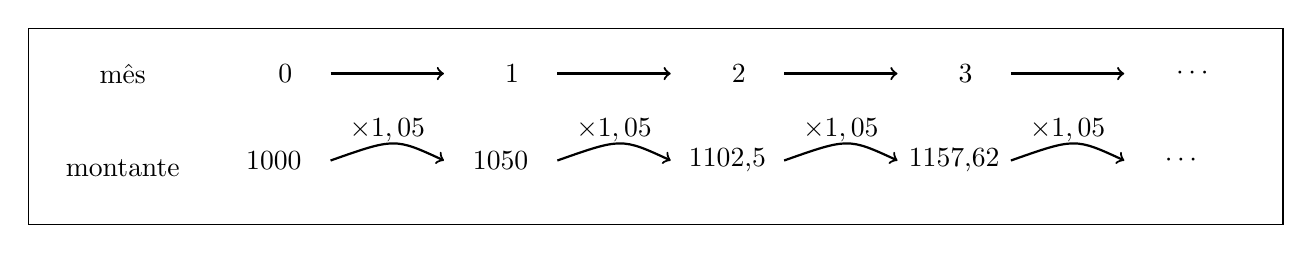
\begin{tikzpicture}[scale=0.48]
\node[black] at (-2,2) {mês};
\node[black] at (-2,-0.5) {montante};
\node[black] at (2,-0.3) {1000};
\node[black] at (2.3,2) {0};
\draw[black, thick, ->] (3.5,2) .. controls (5.2,2) .. (6.5,2);
\draw[black, thick, ->] (3.5,-0.3) .. controls (5.2,0.3) .. (6.5,-0.3);
\node[black] at (5,0.5) {$\times1,05$};

\node[black] at (8,-0.3) {1050};
\node[black] at (8.3,2) {1};
\draw[black, thick, ->] (9.5,2) .. controls (11.2,2) .. (12.5,2);
\draw[black, thick, ->] (9.5,-0.3) .. controls (11.2,0.3) .. (12.5,-0.3);
\node[black] at (11,0.5) {$\times1,05$};

\node[black] at (14,-0.3) {1102,5};
\node[black] at (14.3,2) {2};
\draw[black, thick, ->] (15.5,2) .. controls (17.2,2) .. (18.5,2);
\draw[black, thick, ->] (15.5,-0.3) .. controls (17.2,0.3) .. (18.5,-0.3);
\node[black] at (17,0.5) {$\times1,05$};

\node[black] at (20,-0.3) {1157,62};
\node[black] at (20.3,2) {3};
\draw[black, thick, ->] (21.5,2) .. controls (23.2,2) .. (24.5,2);
\draw[black, thick, ->] (21.5,-0.3) .. controls (23.2,0.3) .. (24.5,-0.3);
\node[black] at (23,0.5) {$\times1,05$};

\node[black] at (26,-0.3) {$\cdots$};
\node[black] at (26.3,2) {$\cdots$};

\draw (28.7,3.2) -- (28.7,-2) -- (-4.5,-2) -- (-4.5,3.2) -- (28.7,3.2);
\end{tikzpicture}
\caption{O crescimento com juros compostos.}
\end{figure}
  

\begin{Recomenda}{Logaritmos - introdução}
{Indica-se que o/a professor/a desenvolva com os estudantes a evolução  do capital apresentando os dados da Figura 1.1 e questione o tempo para que o montante seja de $R\$1.102{,}50$. Espera-se que os estudantes relacionem o número de meses com as multiplicações repetidas, obtendo
\begin{align*} 
1^o \mbox{m\^es} - &1000 \times 1,05 = 1050\\
2^o \mbox{m\^es} - &(1000 \times 1,05) \times 1,05\\
& = 1000 \times (1,05)^2 = 1102,50.
\end{align*}
O/A professora pode, recordando as propriedades da potenciação, ressaltar que os montantes correspondentes aos meses seguintes são 
$1000 \times (1,05)^3$, $1000 \times (1,05)^4$ e assim por diante.}
{1}{1}
\end{Recomenda}

Muitas vezes estamos interessados em saber quanto tempo, ou quantos períodos são necessários para que determinada quantia seja atingida. Na situação acima, por exemplo, quantos meses seriam necessários para atingirmos R\$ $1.102{,}5$? Vemos na sequência de montantes, que seriam necessários dois meses para isso.

\begin{Recomenda}{Para Refletir}
{Numa segunda etapa, indica-se a reflexão, em grupo, com os estudantes sobre o tempo que seria necessário para que um valor fora da progressão fosse atingido (no quadro para refletir). Aqui esperam-se respostas informais e talvez até algum debate entre "os ajustes ocorrem apenas mensalmente"\, e "um valor entre 2 e 3", o que pode auxiliar no desenvolvimento da argumentação da competência 3 da BNCC. Pode-se aproveitar a oportunidade para destacar que o acréscimo não é de 50 reais por mês, ressaltando a diferença entre juro simples e composto (que é o mais frequente).}
{1}{1}
\end{Recomenda}
\begin{reflection}
Para atingirmos $R\$1.150{,}00$ precisaríamos de quanto tempo? Por que não obtemos exatamente esse valor em 3 meses?
\end{reflection}
\begin{resposta}{Para Refletir}  %% Texto inferior
{Para 2 meses o montante está em $1102,50$. Contudo para 3 meses o montante está em R$\$ 1557{,}62$. Portanto, se houver a correção em períodos fracionários, serão necessários menos de 3 meses e mais do que 2 meses. Se não houver correção fracionária é necessário esperar 3 meses e o montante ultrapassa valor inicialmente buscado. O fato dos juros serem compostos mês a mês leva a não aplicação de juros simples e a não aplicação do acréscimo de simplesmente R$\$50{,}00$ mensais. Por isso não chega-se ao valor exato de R$\$1.150{,}00$.}
{1}{0}
\end{resposta}

%\begin{description}
%\item[Teorema]
%\leavevmode\phantomsection\label{\detokenize{AF107-0:term-grandezas-diretamente-proporcionais}}
%Diz-se que \textbf{duas grandezas são diretamente proporcionais} quando elas se correspondem de tal modo que, multiplicando-se uma quantidade de uma delas por um número real, a quantidade correspondente da outra fica multiplicada pelo mesmo número, sempre que os resultados dessas multiplicações fizerem sentido no contexto observado.
%\[\begin{array}{ccc}
%X\quad &\overline{\quad \quad \quad}& \quad Y \\
%k\cdot X \quad &\overline{\quad \quad \quad}& \quad k\cdot Y
%\end{array}\]
%\end{description}

Utilize a tabela a seguir para resolver as atividades propostas:

\begin{table}[!htb]
\centering
\begin{tabular}{|c||lllllllllll|}
\hline
 & \multicolumn{11}{c|}{Expoentes}\\
 \hline                                                    Bases & \cellcolor[HTML]{00A59D}0 & \cellcolor[HTML]{00A59D}1 & \cellcolor[HTML]{00A59D}2 & \cellcolor[HTML]{00A59D}3 & \cellcolor[HTML]{00A59D}4 & \cellcolor[HTML]{00A59D}5 & \cellcolor[HTML]{00A59D}6 & \cellcolor[HTML]{00A59D}7 & \cellcolor[HTML]{00A59D}8 & \cellcolor[HTML]{00A59D}9 & \cellcolor[HTML]{00A59D}10 \\
\hline \hline
\cellcolor[HTML]{EFEFEF} 1,01 & 1                         & 1,01                      & 1,0201                    & 1,030 & 1,040               & 1,051             & 1,061 & 1,072 & 1,082         & 1,093         & 1,104          \\
\cellcolor[HTML]{EFEFEF}{\color[HTML]{000000} 1,1}  & 1                         & 1,1                       & 1,21                      & 1,331                     & 1,464                   & 1,610                   & 1,771                & 1,948                 & 2,143                & 2,357              & 2,593               \\
\cellcolor[HTML]{EFEFEF}{\color[HTML]{000000} 2}    & 1                         & 2                         & 4                         & 8                         & 16                        & 32                        & 64                        & 128                       & 256                       & 512                       & 1024                       \\
\cellcolor[HTML]{EFEFEF}{\color[HTML]{000000} 3}    & 1                         & 3                         & 9                         & 27                        & 81                        & 243                       & 729                       & 2187                      & 6561                      & 19683                     & 59049                      \\ \hline
\end{tabular}
\caption{Potências dos números 1,01; 1,1; 2 e 3.} \label{tabela_Potencias}
\end{table}


\begin{task}{Dívida no cartão}\label{divida_cartao}
Um pessoa tem uma dívida de R\$ $10.000{,}00$ no cartão de crédito, que cobra juros de 10\% ao mês. Se essa dívida não for amortizada, em quantos meses ela ultrapassará R\$ $15.000{,}00$? E $R\$ 20.000{,}00$? E $R\$ 25.000{,}00$?
\end{task}

\begin{task}{Bactérias no leite}
Uma população de uma determinada bactéria contamina um copo de leite à temperatura ambiente. Suponha que o leite seja considerado impróprio para o consumo se a população do copo for maior ou igual a 16.200 indivíduos. A população de bactérias tem, inicialmente, 200 indivíduos e sua população triplica a cada hora até atingir 40.000 indivíduos. Em quanto tempo a população atingirá 16.200 indivíduos?
\end{task}

\begin{Recomenda}{Atividades}
{Após essa introdução indica-se que seja dado tempo aos estudantes para resolver as atividades em duplas ou trios utilizando a tabela apresentada no livro texto. Para utilizar a tabela é necessária a ligação entre o número de vezes que a multiplicação é aplicada com as potências e o professor pode auxiliar os pequenos grupos a concluir isso, caso tenham dificuldade.}
{1}{0}
\end{Recomenda}
\begin{resposta}{Dívida no cartão} 
{Podemos utilizar a tabela para calcular o montante em cada mês a partir de R$\$10.000{,}00$.
\begin{center}
\begin{tabular}{|l|l|l|l|l|l|}
 \hline                     \cellcolor[HTML]{00A59D}  $0$ & \cellcolor[HTML]{00A59D} $1$ & \cellcolor[HTML]{00A59D} $2$ & \cellcolor[HTML]{00A59D}  $3$ & \cellcolor[HTML]{00A59D} $4$ & \cellcolor[HTML]{00A59D} $5$ \\
\hline
$10000$ & $11000$ & $12100$ & $13310$ & $14640$ & $16100$ \\
\hline
\end{tabular}
\begin{tabular}{|l|l|l|l|l|}
 \hline                     \cellcolor[HTML]{00A59D}  $6$ & \cellcolor[HTML]{00A59D} $7$ & \cellcolor[HTML]{00A59D} $8$ & \cellcolor[HTML]{00A59D} $9$ & \cellcolor[HTML]{00A59D} $10$\\
\hline
$177710$ & $19480$ & $21430$ & $23570$ & $25930$\\
\hline
\end{tabular}
\end{center}
Assim atingimos R$\$15.000{,}00$, R$\$20.000{,}00$ e R$\$25.000{,}00$ em, respectivamente 5, 8 e 10 meses.}
{1}
\end{resposta}

\begin{resposta}{Bactérias no Leite} 
{A evolução do número de bactérias pode ser tabelado
\begin{center}
\begin{tabular}{||c|l|l|}
 \hline                     \cellcolor[HTML]{00A59D}  Tempo (em horas) & \cellcolor[HTML]{00A59D} Evolução das Bactérias & \cellcolor[HTML]{00A59D}População \\
\hline \hline
\cellcolor[HTML]{EFEFEF} $0$ & $200$                         & $200$\\
\cellcolor[HTML]{EFEFEF} $1$ & $200 \times 3$                & $600$\\
\cellcolor[HTML]{EFEFEF} $2$ & $200 \times 3^2$             & $1800$\\
\cellcolor[HTML]{EFEFEF} $3$ & $200 \times 3^3$             & $5400$\\
\cellcolor[HTML]{EFEFEF} $4$ & $200 \times 3^4$            & $16200$\\
\hline
\end{tabular}
\end{center}
A população atinge 16200 indivíduos após 4 horas.}
{0}{0}
\end{resposta}

\begin{task}{Economizando para uma viagem}
Rebeca recebeu de sua avó paterna uma herança em dinheiro no valor de $R\$ 40.000{,}00$. Ela pretende utilizar esse dinheiro para conhecer a Inglaterra e o pacote de viagens que ela deseja custa $R\$ 44.000{,}00$. Aplicando o valor da herança a juro de $1\%$ ao mês, quantos meses levará Rebeca para conseguir o valor desejado e realizar seu sonho?
\end{task}
\begin{resposta}{Economizando para uma viagem} 
{Calculando os montantes mês a mês, vemos que Rebeca precisará esperar 10 meses.
\begin{center}
\begin{tabular}{|c|l|l|}
 \hline                     \cellcolor[HTML]{00A59D}  Meses & \cellcolor[HTML]{00A59D} Evolução do montante & \cellcolor[HTML]{00A59D}Montante \\
\hline \hline
\cellcolor[HTML]{EFEFEF} $0$ & $40000$                         & $40000$\\
\cellcolor[HTML]{EFEFEF} $1$ & $40000 \times 1,01$                & $40400$\\
\cellcolor[HTML]{EFEFEF}  & \vdots             & \vdots\\
\cellcolor[HTML]{EFEFEF} $9$ & $40000 \times (1,01)^{9}$             & $43720$\\
\cellcolor[HTML]{EFEFEF} $10$ & $40000 \times (1,01)^{10}$             & $44160$\\
\hline
\end{tabular}
\end{center}}
{0}{1}
\end{resposta}


\arrange{logaritmos}
\label{organizando-as-ideias-logaritmos}

Problemas que envolvem a busca de expoentes, como os calculados nas atividades acima, aparecem com frequência em diversos contextos da matemática e suas aplicações. A esses expoentes damos o nome de logaritmos.


Por exemplo, 3 é o expoente ao qual precisamos elevar a base 2 para obter 8. Dizemos assim que o \textit{o logaritmo de 8 em base 2} é 3 e escrevemos $\log_2 8 = 3$. De modo geral definimos:
\begin{Recomenda}{Apresentando o conceito}
{Indica-se que o/a professor/a ressalte que as incógnitas buscadas nas atividades eram expoentes e, então, apresente a definição formal de logaritmo. Em seguida pode-se ilustrar como o conceito estava sendo utilizado nas atividades anteriores através do exemplo "Identificando os logaritmos", contudo pode ser necessário reforçar que os valores encontrados na tabela como resposta eram aproximações superiores para os logaritmos, pois correspondiam ao mês em que o respectivo valor era ultrapassado.}
{1}{1}
\end{Recomenda}

\begin{description}
\item[Definição]
Para dois números reais $a$ e $b$ positivos, o \textit{logaritmo de a em base b}, que denotamos $\log_b a$, é o expoente ao qual a base $b$ deve ser elevada para obtermos $a$. Assim $c=\log_b a$ se, e somente se, $b^c=a$.
\end{description}

\begin{observation}{}
Quando escrevemos $c = \log_b a$, utilizamos os seguintes \textit{nomes} para os números $a,\,b$ e $c$.
\begin{center}
\begin{minipage}{0.3\linewidth}
\begin{flushleft}
- \textcolor{penlaranja}{$a$} é o \textcolor{penlaranja}{\textit{logaritmando}}.

- \textcolor{penaqua}{$b$} é a \textcolor{penaqua}{\textit{base}}.

- \textcolor{penazul}{$c$} é o \textcolor{penazul}{\textit{logaritmo}}.

\end{flushleft}
\end{minipage}
\begin{minipage}{0.3\linewidth}

\Huge $\log$\textcolor{penaqua}{$_b$} \textcolor{penlaranja}{$a$} = \textcolor{penazul}{$c$}

\end{minipage}
\end{center}
\end{observation}
\begin{ObjetivoEsp}{Nomenclaturas}
{Compreender a notação de logaritmo e suas componentes: base e logaritmando.}
{1}
\end{ObjetivoEsp}

Nas atividades anteriores, estávamos interessados nos expoentes em que precisávamos elevar determinadas bases para encontrar alguns valores, ou seja, estávamos procurando determinados logaritmos. Você consegue identificar os logaritmos buscados nessas atividades e os valores encontrados?  

\begin{example}{Identificando os logaritmos}
Na atividade "Dívida no cartão"\, temos os logaritmandos $a=15000/10000=1,5$, $20000/10000=2$ e $25000/10000=2,5$, a base é sempre $b= 1,1$ e as aproximações encontradas na tabela para os logaritmos são $c= 5$, 8 e 10, respectivamente:
\begin{align*}
\log_{1,1} 1,5 &\approx 5,\\ 
\log_{1,1} 2 &\approx 8,\\
\log_{1,1} 2,5 &\approx 10.
\end{align*}
\end{example}

\begin{observation}{}
Assim o logaritmo $c = \log_b a$ é o expoente em que a base precisa ser elevada para obtermos o logaritmando, ou seja $b^{\log_b a}=a$.
\end{observation}

\begin{Recomenda}{Escrevendo os logaritmos}
{Indica-se que seja reforçado com os estudantes que o logaritmo é o expoente, como na observação do primeiro quadro. Então os estudantes podem praticar individualmente a notação na atividade "Escrevendo os logaritmos", que propõem a identificação dos valores obtidos nas atividades anteriores através dos logaritmos.}
{1}
\end{Recomenda}
\begin{task}{Escrevendo os logaritmos}
Identifique nas atividades "Bactérias no leite"\, e "Economizando para uma viagem"\, os logaritmandos, as bases e as aproximações de logaritmos encontradas na tabela como respostas e escreva-os utilizando a notação simbólica $\log_b a \approx c$.
\end{task}


\begin{observation}{}
Cuidado!!! $\log_b a$ é um número, mas $\log_b$ não é. No entanto, para a base 10, existe a convenção de omitirmos a base. Desse modo que $\log 100$ significa $\log_{10} 100$ (que é igual a 2). De modo geral $\log a =\log_{10} a$.
\end{observation}
\begin{Recomenda}{Cuidado!!!}
{Um distrator apontado na literatura para os logaritmos é que os estudantes buscam operar com $\log_b$ como se fosse um número real per si, por isso o quadro de destaque logo após a atividade, que ressalta também a notação especial para base 10.

Pode-se comparar esse caso especial com a raiz quadrada, $\sqrt{a}$, na qual o 2 é omitido.

Dificilmente obtém-se um valor inteiro para um logaritmo em problemas práticos e faz-se necessária a discussão das aproximações. O exemplo estimando logaritmos é conceitualmente um pouco mais elaborado, mas é necessário para dar sentido às aproximações utilizadas.}
{1}
\end{Recomenda}

\begin{task}{Lei de Moore}
Na computação, a Lei de Moore estima como os computadores progridem. Ela prevê que a capacidade computacional dobra a cada 1,5 ano. Para simplificar nossos cálculos, vamos aproximá-la\footnote{Em 5 anos há $3,\overline{3}$ períodos de $1,5$ anos, então o crescimento seria de $2^{3,\overline{3}} = 10,07$, com duas casas decimais.} por um crescimento de 10 vezes a cada 5 anos. Supondo que as previsões de Moore estejam corretas, utilize a notação de logaritmo para representar quantos quinquênios serão necessários para:
\begin{enumerate}
\item a capacidade computacional aumentar 100 vezes,
\item a capacidade computacional aumentar 1000 vezes.
\end{enumerate}
Qual seria a sua estimativa para a quantidade de quinquênios necessários para a que capacidade computacional aumente 1100 vezes?
\end{task}
\begin{ObjetivoEsp}{Lei de Moore e a base 10}
{Resolver um problema contextualizado aplicando a noção de logaritmo.}
{1}
\end{ObjetivoEsp}

\begin{Recomenda}{Lei de Moore e a base 10}
{Em seguida indica-se aos alunos o exercício sobre a Lei de Moore. Ao apresentar a solução deve-se aproveitar a oportunidade para utilizar a notação de base 10 omitindo a base.}
{1}
\end{Recomenda}

\begin{observation}{Nem toda base faz sentido}
Logaritmos de base 1 não fazem sentido! Qual seria $\log_1 3$? Seria o expoente ao qual devemos elevar 1 para obter 3, mas $1^x = 1$ para qualquer número real $x$. Isso nos levará a excluir a base 1 quando enunciarmos os teoremas. Bases negativas também não fazem sentido, pois exponenciais de bases negativas não fazem sentido, como estudado na seção sobre a função exponencial.
\end{observation}

\begin{resposta}{Lei de Moore} 
{Suponhamos que hoje a capacidade computacional seja representada pela constante c. Após 5 anos, teremos $10c$. Após 10 anos, teremos $10 \times (10c) = c \times 10^2$. Após $t$ quinquênios , teremos $c \times 10^t$
\begin{enumerate} 
\item Queremos chegar a 100 vezes o que é hoje, ou seja, queremos
$$
t = \log 100 = \log_{10} 100  = 2.
$$
\item Queremos chegar a 1000 vezes o que é hoje, ou seja, queremos
$$
t = \log 1000 = \log_{10} 1000  = 3.
$$
\end{enumerate}}
{1}
\end{resposta}

\begin{Recomenda}{Estimando logaritmos}
{Dificilmente obtém-se valores inteiros para logaritmos em problemas práticos e faz-se necessária a discussão das aproximações. O exemplo estimando logaritmos é conceitualmente um pouco mais elaborado, mas é necessário para dar sentido às aproximações utilizadas.}
{1}
\end{Recomenda}
\begin{example}{Estimando logaritmos}
Nem sempre conseguimos calcular um logaritmo exatamente e precisamos aproximá-lo. Por exemplo sabemos que $\log_5 25 = 2$ e $\log_5 125 = 3$, porque $5^2=25$ e $5^3 = 125$. Mas qual seria o valor de $\log_5 100$? Ou seja, qual o expoente que devemos elevar $5$ para obtermos $100$? Do nosso estudo das funções exponenciais, sabemos que $5^x$ é crescente (pois a base é maior do que 1). Como $25 < 100$, o expoente em que precisamos elevar $5$ para obtermos $100$ é maior do que $2$, ou seja $\log_5 100 >2$. De modo análogo, como $125 > 100$, temos $\log_5 100<3$. Assim sabemos que $2<\log_5 100<3$.
\begin{center}
\begin{tikzpicture}[scale=1.5]
\draw[black] (1,0) -- (6,0);
\draw[black] (2,-0.1) -- (2,0.1);
\draw[black] (5,-0.1) -- (5,0.1);
\draw[black] (3.5,-0.1) -- (3.5,0.1);
\node[black] at (2,-0.5) {$2$};
\node[black] at (3.5,-0.5) {$2{,}5$};
\node[black] at (5,-0.5) {$3$};
\draw[penaqua] (4.58,0) -- (4.58,0.2);
\node[penaqua] at (4.58,0.5) {$\log_5 100$};
\end{tikzpicture}
%\captionof{figure}{O $\log_5 100$ está no intervalo $(2,3)$.}
\end{center}
Assim a distância do $\log_5 100$ para $2$ ou para $3$ é menor do que $1$ e poderíamos aproximá-lo por $2$ ou $3$ com erro menor do que $1$. Poderíamos, também, aproximar $\log_5 100$ por $2{,}5$ com erro menor do que $0{,}5$. 
\end{example}

\begin{Recomenda}{Praticando}
{Essa seção contém exercícios que podem ser resolvidos fora da sala da aula.\\
Os primeiros pretendem que os cálculos sejam apoiados na definição de logaritmo.\\
Os últimos têm como propósito a utilização de alguma ferramenta (a tabela ou o applet de GeoGebra) para o cálculo de logaritmos. Na prática, atualmente, recorre-se frequentemente à calculadora para o cálculo de logaritmos e o exercício inicia o estudante a essa prática.\\
Antigamente recorria-se a tabelas ou réguas de cálculo para encontrar-se os valores de logaritmos e mais informações históricas sobre essas práticas podem ser encontradas nas seções \textit{Para saber +: sem ferramentas de cálculo} e \textit{Para saber +: a régua de cálculo}.}
{1}
\end{Recomenda}

\practice{logaritmos}
\begin{ObjetivoEsp}{Cálculos sem a calculadora}
{Praticar a definição de logaritmo e o seu cálculo através do conceito propriamente dito.}
{1}
\end{ObjetivoEsp}

\begin{resposta}{Sem a calculadora} 
{\begin{enumerate}
\item $\log_2 8 = 3$ pois $2^3 = 8$;
\item $\log_{1/2} 32 = -5$ pois $(1/2)^{-5} = 2^5 = 32$;
\item $\log 1000= 3$ pois $10^3 = 1000$;
\item Como $2^3=8 <10 <2^4 =16$, temos que $\log_2 10$ pode ser aproximado por 3 ou 4 com erro menor do que 1;
\item Como $10 ^2 = 100 < 113 < 10^3 = 1000$, temos que $\log 113$ pode ser aproximado por 2 ou 3 com erro menor do que 1;
\item Como $3^3= 27 <30 <3^4 =81$, temos que $\log_3 30$ pode ser aproximado por 3 ou 4 com erro menor do que 1.
\end{enumerate}}
{1}
\end{resposta}

\begin{task}{cálculos sem a calculadora}

Calcule exatamente ou encontre um número natural que aproxime, com erro menor do que 1, os seguintes logaritmos (justificando as suas respostas):
\begin{multicols}{2}
\begin{enumerate}
\item $\log_2 8$;
\item $\log_{1/2} 32$;
\item $\log 1000$;
\item $\log_2 10$;
\item $\log 113$;
\item $\log_3 30 $.
\end{enumerate}
\end{multicols}
\end{task}



Calcular logaritmos manualmente pode ser muito laborioso, por isso utiliza-se, preferencialmente, ferramentas digitais. Utilize o applet do geogebra\footnote{Pode ser necessário utilizar o celular deitado para que apareçam os controles deslizantes.} acessível em \url{https://www.geogebra.org/classic/ug8fmvtc} ou no QR code abaixo, para realizar os cálculos abaixo.
\begin{figure}[H]
\centering
\noindent\fbox{\includegraphics[height=25mm]{{AelevadoB}.png}}\hspace{15mm}
\includegraphics[height=30mm]{QRcode_AelevadoB.png}
\caption{Ilustração do applet e QR code.}
\end{figure}


\begin{ObjetivoEsp}{Com ferramentas computacionais}
{Encontrar o valor dos logaritmos em bases distintas através de tabelas e/ou de aplicativos.}
{1}
\end{ObjetivoEsp}
\begin{resposta}{Com ferramentas computacionais} 
{\begin{enumerate}
\item $\log_{1,41} 4 \approx 4,03$;
\item $\log_{2,71} 4 \approx 1,39$;
\item $\log_{2} 5 \approx 2,32$;
\item $\log_{4} 7 \approx 1,4$;
\item $\log_{2,71} 9 \approx 2,2$;
\item $\log_{3} 7 \approx 1,77$.
\end{enumerate}}
{1}
\end{resposta}

\begin{task}{cálculos com ferramentas computacionais}

No applet do geogebra, mova os controles deslizantes das variáveis “a” e “b” e encontre um valor aproximado (com até duas casas decimais) para:
\begin{multicols}{2}
\begin{enumerate}
\item $\log_{1,41} 4$;
\item $\log_{2,71} 4$;
\item $\log_2 5$;
\item $\log_4 7$;
\item $\log_{2,71} 9$;
\item $\log_3 7$.
\end{enumerate}
\end{multicols}
\end{task}


Se não tiver acesso ao applet, as atividades podem ser resolvidas utilizando a tabela\footnote{Utilizamos as bases 1,41 pois elas aproximam $\sqrt{2} \approx 1,41$ e $e \approx 2,71$, que podem ser interessantes em outros problemas.} abaixo.
% Please add the following required packages to your document preamble:
% \usepackage[table,xcdraw]{xcolor}
% If you use beamer only pass "xcolor=table" option, i.e. \documentclass[xcolor=table]{beamer}
\begin{table}[H]
\centering
\begin{tabular}{|c||llllllllll|}
\cline{2-11}
\multicolumn{1}{c|}{}                                & \multicolumn{10}{c|}{Logaritmando}                                                                                                                                                                                                                                                     \\ \hline
Base                                                 & \cellcolor[HTML]{00A59D}1 & \cellcolor[HTML]{00A59D}2 & \cellcolor[HTML]{00A59D}3 & \cellcolor[HTML]{00A59D}4 & \cellcolor[HTML]{00A59D}5 & \cellcolor[HTML]{00A59D}6 & \cellcolor[HTML]{00A59D}7 & \cellcolor[HTML]{00A59D}8 & \cellcolor[HTML]{00A59D}9 & \cellcolor[HTML]{00A59D}10 \\ \hline\hline
\cellcolor[HTML]{EFEFEF}{\color[HTML]{000000} 1,41} & 0                         & 2,02                         & 3,2                      & 4,03                         & 4,68                      & 5,21                      & 5,66                      & 6,05                         & 6,34                      & 6,7
                       \\
\cellcolor[HTML]{EFEFEF}{\color[HTML]{000000} 2}     & 0                         & 1                         & 1,58                      & 2                         & 2,32                      & 2,58                      & 2,81                      & 3                         & 3,17                      & 3,32                       \\
\cellcolor[HTML]{EFEFEF}{\color[HTML]{000000} 2,71} & 0                         & 0,7                      & 1,1                       & 1,39                      & 1,61                      & 1,8                      & 1,95                      & 2,09                      & 2,2                       & 2,31                        \\
\cellcolor[HTML]{EFEFEF}{\color[HTML]{000000} 3}                             & 0                         & 0,63                      & 1                         & 1,26                      & 1,46                      & 1,63                      & 1,77                      & 1,89                      & 2                         & 2,1                        \\
\cellcolor[HTML]{EFEFEF}{\color[HTML]{000000} 4}     & 0                         & 0,5                       & 0,79                      & 1                         & 1,16                      & 1,29                      & 1,4                       & 1,5                       & 1,58                      & 1,66                       \\ \hline
\end{tabular}
\caption{Logaritmos nas bases $1{,}41$; $2$; $2{,}71$; $3$ e $4$.} \label{tabela_logs}
\end{table}





\exercise

\begin{ObjetivoEsp}{Exercícios}
{\begin{itemize}
\item Consolidar o conceito de logaritmo através do cálculo por meio da definição.
\item Reconhecer os papeis da base, do logaritmando e do logaritmo e calcular os logaritmos.
\end{itemize}}
{1}
\end{ObjetivoEsp}


\begin{Recomenda}{Exercícios p.5}
{Essa seção contém exercícios que podem ser resolvidos fora da sala da aula.\\
As atividades pretendem fixar os conceitos adquiridos e, por isso trazem novamente exercícios para os quais são necessários cálculos pela definição e cálculos com ferramentas (computacionais ou tabelas).}
{1}
\end{Recomenda}

\begin{resposta}{\ref{calcule} - Calcule} 
{\begin{enumerate}[label=\alph*)]
\item $\log_2 64 = 6$, pois $2^6 = 64$;
\item $\log_{3} 27 = 3$, pois $3^{3} = 27$;
\item $\log_{3} 81 = 4$, pois $(3)^{4} = 81$;
\item $\log_{1/5} 625 = -4$, pois $(1/5)^{-4} =  5^4 = 625$;
\item $\log 0,0001 = -4$, pois $10^{-4} =1/10^4 = 0,0001 $;
\item $\log_{27} 243 = 5/3$, pois $27=3^3$ e $243 = 3^5$, assim $27^{5/3} =(3^3)^{5/3}= 3^5 = 243$;
\item $\log_{1/4} 32 = 5/2$, pois $4=2^2$ e $32 = 2^5$, assim $4^{5/2} =(2^2)^{5/2}= 2^5 = 32$.
\end{enumerate}}
{1}
\end{resposta}

\begin{resposta}{\ref{identifique} - Identifique} 
{\begin{enumerate}[label=\alph*)]
Não há cálculos a realizar, apenas encontrar os valores na tabela 2 ou através do applet. 
\item $x$ é a base, que deve igualar 2,71;
\item $x$ é o logaritmando, que deve igualar 8;
\item $x$ é a base, que deve igualar 1,41;
\item $x$ é o logaritmo, que deve igualar 1,46;
\item $x$ é o logaritmo, que deve igualar 0;
\item $x$ é o logaritmando, que deve igualar 6.
\end{enumerate}}
{1}
\end{resposta}

\begin{ObjetivoEsp}{Problemas contextualizados}
{Resolver questões práticas envolvendo logaritmos no contexto de matemática financeira, auxiliando no desenvolvimento da habilidade

\textit{EM13MAT305 - Resolver e elaborar problemas com funções logarítmicas no contexto de matemática financeira.}}
{1}
\end{ObjetivoEsp}

\begin{Recomenda}{Problemas contextualizados}
{Os exercícios contextualizados retornam ao contexto importantíssimo de matemática financeira, colaborando no desenvolvimento da habilidade EM13MAT305, apesar de a formulação não trazer explicitamente uma função, pois temos implicitamente montantes que dependem de variáveis de tempo.}
{1}
\end{Recomenda}

\begin{enumerate}


\item {}\label{calcule}

Calcule, usando a definição, os seguintes logaritmos:
\begin{enumerate}
\item $log_2 64$;
\item $log_3 27$;
\item $log_3 81$;
\item $log_{1/5} 625$;
\item $log 0,0001$;
\item $log_{27} 243$;
\item $log_{1/4} 32$.
\end{enumerate}



\item{}\label{identifique}

Identifique, em cada caso, se $x$ é a base, o logaritmo  ou o logaritmando e utilize o applet do geogebra ou a Tabela \ref{tabela_logs} para encontrar o valor de $x$:
\begin{enumerate}
\item $log_{x} 10 = 2{,}31$;
\item $log_{2{,}71} x = 2{,}09$;
\item $log_x 8 = 6{,}05$;
\item $log_3 5 =x$;
\item $log_{2{,}71} 1= x$;
\item $log_{2} x= 2{,}58$.
\end{enumerate}
\end{enumerate}


Se não tiver acesso ao applet, as atividades seguintes podem ser resolvidas utilizando a tabela seguinte.
% Please add the following required packages to your document preamble:
% \usepackage[table,xcdraw]{xcolor}
% If you use beamer only pass "xcolor=table" option, i.e. \documentclass[xcolor=table]{beamer}
\begin{table}[H]
\centering
\begin{tabular}{|c||llllllllll||}
\hline
\multicolumn{10}{|c|}{Expoentes}\\
\hline
\cellcolor[HTML]{00A59D}1 & \cellcolor[HTML]{00A59D}2 & \cellcolor[HTML]{00A59D}3 & \cellcolor[HTML]{00A59D}4 & \cellcolor[HTML]{00A59D}5 & \cellcolor[HTML]{00A59D}6 & \cellcolor[HTML]{00A59D}7 & \cellcolor[HTML]{00A59D}8 & \cellcolor[HTML]{00A59D}9 & \cellcolor[HTML]{00A59D}10 \\ \hline\hline
\cellcolor[HTML]{EFEFEF}{\color[HTML]{000000} 1,0035}  & 1,007                         & 1,0105                         & 1,014                      & 1,0176                         & 1,0211                      & 1,0247                      & 1,0283                      & 1,0319                         & 1,035                                           \\
\cellcolor[HTML]{EFEFEF}{\color[HTML]{000000} 1,03}   & 1,06                         & 1,092                      & 1,125                         & 1,159                      & 1,194                      & 1,229                      & 1,266                         & 1,304                      & 1,343                       \\
\cellcolor[HTML]{EFEFEF}{\color[HTML]{000000} 1,14}  & 1,299                      & 1,481                       & 1,688                      & 1,925                      & 2,194                      & 2,502                      & 2,852                      & 3,251                       & 3,707                        \\ \hline
\end{tabular}
\caption{Potências de $1,0035$, $1,03$ e $1,14$.} \label{tabela_potencias2}
\end{table}


\begin{enumerate}
\setcounter{enumi}{2}
\item {}\label{poupancaBrasil}

A poupança é o tipo de investimento mais popular no Brasil. Esse tipo de aplicação tem baixo rendimento, contudo não oferece riscos. Em 2019 o rendimento da poupança atingiu a média de $0{,}35\%$ ao mês. Um investidor que aplicou R$\$ 5000{,}00$ na poupança, à taxa de juros compostos de $0{,}35\%$ ao mês, obteve um montante de R$\$ 5141{,}72$. Por quanto tempo esse dinheiro esteve investido?


\item {} \label{cartaoCredito}

A taxa média de juros do rotativo do cartão no Brasil é de $352,76\%$ ao ano, que é aproximadamente de $14\%$ ao mês, uma das taxas mais elevadas no mundo, segundo levantamento da Proteste para o ano de 2018. Para se ter um comparativo, ainda de acordo com a Proteste, o percentual de juros do crédito anual na Argentina é de $47,40\%$, que é aproximadamente $3\%$ ao mês.\\
Uma pessoa que devia R$\$ 1.200,00$ no cartão de crédito, com uma taxa de $14\%$ ao mês, ficou impossibilitada de pagar sua fatura até o valor da dívida ficar em R$\$ 2.310,50$. Quanto tempo ela ficou sem pagar a fatura? Se a dívida tivesse a taxa média da Argentina, de $3\%$ ao mês, a que valor ela chegaria no mesmo período?

\end{enumerate}
\begin{resposta}{\ref{poupancaBrasil} - Poupança} 
{Devemos encontrar $t$ de forma que
\begin{align*}
& 5000 \times (1,0035)^t = 5141,72
\Leftrightarrow (1,0035)^t = 1,028388.
\end{align*}
Pela tabela vemos que t = 8 meses.}
{1}
\end{resposta}
\begin{resposta}{\ref{cartaoCredito} - Cartão de crédito} 
{O tempo que a pessoa ficou sem pagar é calculado por
\begin{align*}
t =& \log_{1{,}14} (2310{,}50/1200)= \log_{1{,}14} 1{,}925.
\end{align*}
De acordo com a tabela $t = 5$ meses.

Se a dívida tivesse a taxa de 3$\%$,
\begin{align*}
D =& 1200 \times (1,03)^5= 1391,
\end{align*}
ela estaria em R$\$1391{,}12$ após 5 meses.}
{0}
\end{resposta}

\explore{Logaritmo do produto}\label{prod_logaritmo}

\begin{ObjetivoEsp}
{Logaritmo do Produto}
{\begin{itemize}
\item Observar padrões nos valores dos logaritmos quando os logaritmandos são multiplicados por um número natural.
\item Inferir a propriedade do logaritmo do produto a partir da observação dos valores tabelados.
\item Sintetizar a propriedade do logaritmo a partir da sua validade nos exemplos específicos.
\end{itemize}}
{1}
\end{ObjetivoEsp}

Existem algumas propriedades que auxiliam na resolução de problemas envolvendo logaritmos. Uma dessas propriedades é chamada de logaritmo do produto e estudaremos ela a seguir.  Vamos explorar os valores dos logaritmos e buscar relações entre eles.%Veremos que essas propriedades estão relacionadas com o surgimento dos logaritmos e sua aplicação inicial: facilitar cálculos de multiplicação.

\begin{Recomenda}
{Logaritmo do Produto}
{A \textit{descoberta} de uma propriedade acontece, muitas vezes, através da observação de sua validade em exemplos específicos. Acreditamos que auxiliar os estudantes a descobrir a propriedade pode ser preferível ao simplesmente apresentá-la. Levamos isso ao encontro da proposta da Educação Matemática Realista, no sentido de partir de raciocínios informais e buscar amadurecê-los até a formalização.

Nesse espírito propõe-se a atividade \textit{"Relações entre os logaritmos"}, com o intuito de induzi-los a observar a propriedade naturalmente. Segue-se com um \textit{Para refletir}, que pode ser realizado como uma discussão em grupo, moderada pelo/a professor/a.}
{1}
\end{Recomenda}

Iniciamos utilizando a tabela de potências racionais de 2 a seguir para buscar padrões nos logaritmos de base 2. Os expoentes são aproximações dos logaritmos dos naturais na coluna ao lado, com erro menor do que $0,01$.

\begin{table}[H]
\centering
\begin{tabular}{|l|l||l|l||l|l|}
\hline
\cellcolor[HTML]{00A59D} $2^{\log_2 n}$ & \cellcolor[HTML]{00A59D}  $n$ & \cellcolor[HTML]{00A59D} $2^{\log_2 n}$ & \cellcolor[HTML]{00A59D}  $n$ &
\cellcolor[HTML]{00A59D} $2^{\log_2 n}$ & \cellcolor[HTML]{00A59D}  $n$ \\
\hline $2^0$ & $1$ & $2^{3,46}$ & $11$ & $2^{4,39}$ & $21$ \\
\hline $2^1$ & $2$ & $2^{3,58}$ & $12$ & $2^{4,46}$ & $22$ \\
\hline $2^{1,58}$ & $3$ & $2^{3,7}$ & $13$ & $2^{4,52}$ & $23$ \\
\hline $2^2$ & $4$ & $2^{3,81}$ & $14$ & $2^{4,58}$ & $24$ \\
\hline $2^{2,32}$ & $5$ & $2^{3,9}$ & $15$ & $2^{4,64}$ & $25$ \\
\hline $2^{2,58}$ & $6$ & $2^4$ & $16$ & $2^{4,7}$ & $26$ \\
\hline $2^{2,81}$ & $7$ & $2^{4,08}$ & $17$ & $2^{4,75}$ & $27$ \\
\hline $2^3$ & $8$ & $2^{4,16}$ & $18$ & $2^{4,81}$ & $28$ \\
\hline $2^{3,16}$ & $9$ & $2^{4,24}$ & $19$ & $2^{4,85}$ & $29$ \\
\hline $2^{3,32}$ & $10$ & $2^{4,32}$ & $20$ & $2^{4,9}$ & $30$ \\
\hline
\end{tabular}
\caption{Expoentes de $2$ aproximando os naturais de $1$ à $30$}\label{potencias2_log}
\end{table}

\begin{resposta}{Relações entre os logaritmos}
{\begin{itemize}
\item $\log_2 2 = 1$, $\log_2 4 = 2$, $\log_2 8 = 3$ e $\log_2 16 = 4$.
\item $\log_2 3 \approx 1{,}58$, $\log_2 6 \approx 2{,}58$, $\log_2 12 \approx 3{,}58$ e $\log_2 24 \approx 4{,}58$.
\item $\log_3 3 = 1$, $\log_3 9 = 2$ e $\log_3 27 = 3$.
\item $\log_2 3 \approx 1{,}58$, $\log_2 5 \approx 2{,}32$ e $\log_2 15 \approx 3{,}9$.
\end{itemize}}
{0}
\end{resposta}

\begin{resposta}{Para refletir}
{Espera-se respostas dos estudantes como "Multiplicar por dois aumenta o resultado em 1 no item a), e também no b)", "Multiplicar por três aumenta o resultado em 1 no item c)". No item d) pode ser necessária a mediação do/a professor/a para observar-se que $\log _2 15$ é a soma de $\log _2 3$ e $\log _2 5$. A conclusão da atividade poderia ser em raciocínios como "Ao multiplicarmos (o logaritmando) soma-se o valor do logaritmo", contudo pode ser necessária a mediação novamente.}
{1}
\end{resposta}

\begin{task}{Relações entre os logaritmos}
Utilize a Tabela \ref{potencias2_log} para encontrar os valores (aproximados) dos seguintes logaritmos em seu caderno:
\begin{enumerate}
\item $\log_2 2$, $\log_2 4$, $\log_2 8$ e $\log_2 16$.
\item $\log_2 3$, $\log_2 6$, $\log_2 12$ e $\log_2 24$.
\item $\log_2 3$, $\log_2 9$ e $\log_2 27$.
\item $\log_2 3$, $\log_2 5$ e $\log_2 15$.
\end{enumerate}
\end{task}

\begin{reflection}
No item a), podemos observar que $\log_2 8 = 3 = 1 + 2 = \log_2 2 + \log_2 4$. Você percebe algum padrão nos valores encontrados nos outros itens da atividade \textit{Relações entre os logaritmos}? Observando os valores da tabela para os logaritmos de $a$ e $b$ e o valor do logaritmo de $a \times b$, encontramos alguma relação entre eles? Vamos buscar exemplos na tabela que justifiquem a resposta.
\end{reflection}

\clearmargin

\begin{Recomenda}{Desenvolvimento bacteriano}
{A atividade \textit{"Desenvolvimento bacteriano"} busca destacar a propriedade do produto. Recomenda-se que, ao resolver os exercícios com os estudantes, seja ressaltado que no item b) dobramos o logaritmando e a resposta aumentou em 1, no item c) o logaritmando é multiplicado por 32 e a resposta aumenta em 5, que é $\log_2 32$; e no item d) o logaritmando é multiplicado novamente por 32 e a resposta aumenta em 5 (que é o logaritmo de 32 em base 2).}
{1}
\end{Recomenda}

\begin{task}{Desenvolvimento bacteriano}
Uma espécie de bactéria dobra a população a cada dia e uma cultura tem 100 indivíduos inicialmente. Sabendo que $2^5=32$ e $2^6=64$, vamos estimar quantos dias levará para que a população: 
\begin{enumerate}
\item Chegue a 3200?
\item Chegue a 6400?
\item Chegue a 204800?
\item Chegue a 6553600?
\end{enumerate}
\end{task}

\begin{resposta}{Desenvolvimento bacteriano}
{A população após $n$ meses é $P(n) = 100 \times 2^n$, assim
\begin{enumerate}[label = \alph*)]
\item $3200 = P(n) = 100 \times 2^n \Rightarrow 2^n = 32 \Rightarrow n=5$.
\item $6400 = P(n) = 100 \times 2^n \Rightarrow 2^n = 64 \Rightarrow n=6$.
\item $204800 = P(n) = 100 \times 2^n \Rightarrow 2^n = 2048 = 32 \times 64 \Rightarrow n=5+6=11$.
\item $6553600 = P(n) = 100 \times 2^n \Rightarrow 2^n = 65536 = 2048 \times 32 \Rightarrow n=11+5=16$.
\end{enumerate}}
{0}
\end{resposta}

\arrange{Logaritmo do produto}\label{explore_log_prod}

\begin{ObjetivoEsp}  %% Texto lateral
{Teorema}
{Comprovar a validade da propriedade do logaritmo do produto.}
{1}
\end{ObjetivoEsp}


\begin{Recomenda}{Teoremas}
{Recomenda-se a demonstração da propriedade, pois é saudável ao estudante que questione as informações que lhe são apresentadas, mas que também seja capaz de buscar evidências para sua validade ou não. Também recomenda-se que seja ressaltada a necessidade de questionar as próprias conjecturas e não acreditar em poucos exemplos pontuais como confirmação da validade de fatos.

Por fim a demonstração finaliza a investigação da propriedade e relaciona-se à 5ª competência da BNCC:

\textit{Investigar e estabelecer conjecturas a respeito de diferentes conceitos e propriedades matemáticas, empregando estratégias e recursos, como observação de padrões, experimentações e diferentes tecnologias, identificando a necessidade, ou não, de uma demonstração cada vez mais formal na validação das referidas conjecturas.}}
{1}
\end{Recomenda}

Observamos nas atividades anteriores, que se conhecemos os logaritmos de dois números e queremos calcular o logaritmo do produto deles, basta somar os logaritmos dos dois primeiros números e teremos o logaritmo do produto deles, ou seja:


\begin{description}
\item[Teorema]\label{teo_log_prod}
[do logaritmo do produto] Dados números reais positivos $a,b$ e $c$, com $a \neq 1$, temos que
$$
\log_a(bc) = \log_a b + \log_a c.
$$
\end{description}
\begin{proof}
O logaritmo de $bc$ em base $a$ é, por definição, o expoente ao qual devemos elevar $a$ para obter $bc$. Assim, basta mostrarmos que $a^{\log_a b + \log_a c} =bc$, o que pode calculado lembrando que $a^{\log_a b}=b$ e $a^{\log_a c}=c$:
\begin{align*}
a^{\log_a b + \log_a c} = a^{\log_a b} \times a^{\log_a c} =bc,
\end{align*}
onde utilizamos a propriedade da exponencial que $a^{x+y} = a^{x} \times a^{y}$.
\end{proof}

\begin{observation}{}
Cuidado!!! Um erro comum envolvendo logaritmos é assumir uma espécie de distributividade para eles, que não existe. Ressaltamos que, em geral,
$$
\log_a b + \log_a c \neq \log_a (b +c),
$$
e a propriedade correta é 
$$
\log_a b + \log_a c = \log_a (bc).
$$
Essa equação também mostra que, em geral,
$$
\log_a (bc) \neq \log_a b \log_a c.
$$
\end{observation}

\begin{Recomenda}{Cuidado!!!}
{A literatura sobre o ensino de logaritmos apresentada na introdução traz o diagnóstico: os estudantes buscam tratar "$\log_a$" como um número per si e assumem a validade da distributividade, que é incorreta. Por isso recomenda-se o destaque que tal propriedade não é válida.}
{1}
\end{Recomenda}

Vale uma propriedade análoga para o logaritmo do quociente de dois números.

\begin{ObjetivoEsp}  %% Texto lateral
{Teorema}
{Comprovar a validade da propriedade do logaritmo do quociente.}
{1}
\end{ObjetivoEsp}


\begin{description}
\item[Teorema]\label{teo_log_div}
[do logaritmo do quociente] Dados números reais positivos $a,b$ e $c$, com $a \neq 1$, temos que
$$
\log_a(b/c) = \log_a b - \log_a c.
$$
\end{description}
\begin{proof}
O logaritmo de $b/c$ em base $a$ é, por definição, o expoente ao qual devemos elevar $a$ para obter $b/c$. Assim, basta mostrarmos que $a^{\log_a b - \log_a c} =b/c$, o que pode calculado lembrando que $a^{\log_a b}=b$ e $a^{\log_a c}=c$:
\begin{align*}
a^{\log_a b - \log_a c} = a^{\log_a b} \times a^{-\log_a c} = a^{\log_a b} \times 1/ a^{\log_a c}  =b/c,
\end{align*}
onde utilizamos a propriedade da exponencial que $a^{x-y} = a^{x} \times a^{-y}$ e o fato que $a^{-y}=1/a^y$.
\end{proof}

\begin{Recomenda}{Cuidado!!!}
{Recomenda-se destacar que a soma/subtração de logartimos não é igual ao logaritmo da soma/subtração. A literatura aponta que os estudantes, com frequência, assumem que podem utilizar a "distributividade"\, no logaritmo, que é incorreta.}
{1}
\end{Recomenda}

\begin{observation}{}
Cuidado!!! Um erro comum envolvendo logaritmos é assumir uma espécie de distributividade para eles, que não existe. Ressaltamos que, em geral,
$$
\log_a b - \log_a c \neq \log_a (b - c),
$$
e a propriedade correta é 
$$
\log_a b - \log_a c = \log_a (b/c).
$$
Essa equação também mostra que, em geral,
$$
\log_a (b/c) \neq \log_a b/\log_a c.
$$
\end{observation}

\ifnum \aluno=1
\vspace{0mm}
\else
\vspace{-1mm}
\fi

\begin{Recomenda}{Valores além da tabela}
{Ainda desenvolvendo a investigação das propriedades do logaritmo, chegamos a uma aplicação na matemática, que é o cálculo dos logaritmos de números além daqueles nas tabelas.

Posteriormente, será realizada a exploração dessas propriedades na resolução de problemas práticos, mas, conforme indicado pelos resultados do pisa (\cite{OCDE2016}), a exploração da matemática pura também é importante, inclusive para a resolução de problemas aplicados. Assim, essa etapa do desenvolvimento do conteúdo parece adequada para a exploração dessas propriedades.}
{1}
\end{Recomenda}

\ifnum \aluno=1
\vspace{0mm}
\else
\vspace{-1mm}
\fi


\begin{example}{Valores além da tabela}
Qualquer tabela será limitada, mas podemos utilizar as propriedades dos logaritmos de valores que estão além da tabela. Por exemplo, utilizando a Tabela \ref{potencias2_log}, podemos calcular (aproximações) de logaritmos de números maiores que os tabelados:
$$
\log_2 300 = \log_2 15 \times 20 = \log_2 15 +\log_2 20 \approx 3{,}9 + 4{,}32 = 8{,}22;
$$
ou números fracionários:
$$
\log_2 3{,}5 = \log_2 (7/2) = \log_2 7 -\log_2 2 \approx 2{,}81 -1 = 1{,}81.
$$
\end{example}

\begin{resposta}{Além da tabela}
{\begin{enumerate}
\item $\log_2 64 = \log_2 16 \times 4= \log_2 16 + \log_2 4 \approx 4+2 =6$;
\item $\log_2 48 = \log_2 24 \times 2= \log_2 24 + \log_2 2 \approx 4{,}58+1 =5{,}58;$
\item $\log_2 60 = \log_2 30 \times 2= \log_2 30 + \log_2 2 \approx 4{,}9+1 =5{,}9;$
\item $\log_2 3/2 = \log_2 3 - \log_2 2 \approx 1{,}58-1 =0{,}58;$
\item $\log_2 600/1024 = \log_2 75/128= \log_2 3 \times 25- \log_2 8 \times 16= \log_2 3 + \log_2 25- (\log_2 8 +\log_2 16) \approx 1{,}58 + 4{,}64-(3+4)= 6{,}22-7 = -0{,}78.$
\end{enumerate}}
{1}
\end{resposta}

\ifnum \aluno=1
\vspace{0mm}
\else
\vspace{-3mm}
\fi

\begin{task}{Além da tabela}
Utilize a Tabela \ref{potencias2_log} para encontrar os valores dos seguintes logaritmos:
\begin{enumerate}
\item $\log_2 64$;
\item $\log_2 48$;
\item $\log_2 60$;
\item $\log_2 (3/2)$;
\item $\log_2 (600/1024)$.
\end{enumerate}
\end{task}
\ifnum \aluno=1
\vspace{0mm}
\else
\vspace{-1mm}
\fi

\begin{Recomenda}{Para refletir}
{Recomenda-se a reflexão com os estudantes sobre o logaritmo da potência, que é uma propriedade fundamental na resolução de problemas práticos, pois é amplamente utilizada para "retirar" a variável do expoente de alguma equação. Recomenda-se que a atividade seja desenvolvida como uma discussão em grupo com os estudantes.}
{1}
\end{Recomenda}

\ifnum \aluno=1
\vspace{0mm}
\else
\vspace{-1mm}
\fi


\begin{resposta}{Para refletir}
{Espera-se que os estudantes consigam perceber que o $\log_a b^n$ pode ser obtido pela aplicação repetida do logaritmo do produto. Para isso pode ser necessário que o/a professor/a realize mediação, ressaltando que o significado de $b^n$ como $"b \times b \times b \times \cdots \times b"$. Recomenda-se, que após a discussão e reflexão, seja enunciada a propriedade do logaritmo da potência para esse caso particular, o que é feito na observação seguinte.}
{1}
\end{resposta}

\begin{reflection}
Utilizando a propriedade do logaritmo do produto, você consegue inferir alguma fórmula para calcular o valor de $\log_a b^n$, para $n \in \mathbb{N}$? Vamos buscar um padrão calculando alguns exemplos, como $\log 100$, $\log 100^2$ e $\log 100^3$?
\end{reflection}

\begin{observation}{}
Não apenas para a base $10$, mas para qualquer base $a>0$, $a \neq 1$, logaritmando $b>0$ e $n \in \mathbb{N}$, temos:
$$
\log_a b^n = \underbrace{\log_a b + \log_a b + \cdots + \log_a b}_{n \mbox{ vezes }} = n\log_a b.
$$
\end{observation}

\begin{ObjetivoEsp}  %% Texto lateral
{Casas decimais}
{\begin{itemize}
\item Aplicar a propriedade do logaritmo da potência para encontrar aproximações inteiras de logaritmos.
\item Explorar o conceito de erro nas aproximações dos logaritmos.
\end{itemize}}
{1}
\end{ObjetivoEsp}

\begin{Recomenda}  %% Texto lateral
{Casas decimais}
{Infelizmente o cálculo de logaritmos não produz, com frequência, resultados inteiros ou fracionais. Recomenda-se, por isso, que erros e aproximações sejam discutidos, na medida do possível, conforme for necessário. Também a BNCC recomenda essas considerações na habilidade:

\textbf{(EM13MAT313)} \textit{Utilizar, quando necessário, a notação científica para expressar uma medida, compreendendo as noções de algarismos significativos e algarismos duvidosos, e reconhecendo que toda medida é inevitavelmente acompanhada de erro.}
}
{1}
\end{Recomenda}

\begin{example}{Casas decimais}
Vemos imediatamente, com a propriedade, que $\log 10^n =n$ e podemos usar isso para estimar logaritmos em base 10 com erro menor do que 1 facilmente. Para estimar $\log 378$ podemos perceber que $10^2=100<378<1000=10^3$ e, como a função exponencial de base $10$ é crescente, temos
\begin{align*}
2 < \log 378 < 3,
\end{align*}
e podemos dizer que a parte inteira do $\log 378$ é dois, ou seja $\log 378 = 2{,}\ldots$
\end{example}

\begin{resposta}{Ordens de grandeza}
{\begin{enumerate}
\item Como $10^0=1 < 6{,}7 <10 =10^1$ e $f(t)=10^t$ é crescente, temos que $0 < \log 6{,}7 < 1$ e sua parte inteira (e sua ordem de grandeza) é $0$.
\item Como $10^1=10 < 23 <100 =10^2$ e $f(t)=10^t$ é crescente, temos que $1 < \log 23 < 2$ e sua parte inteira (e sua ordem de grandeza) é $1$.
\item Como $10^2=100 < 179{,}28 <1000 =10^3$ e $f(t)=10^t$ é crescente, temos que $2 < \log 179{,}28 < 3$ e sua parte inteira (e sua ordem de grandeza) é $2$.
\item Como $10^3=1000 < 8341 <10000 =10^4$ e $f(t)=10^t$ é crescente, temos que $3 < \log 8341 < 4$ e sua parte inteira (e sua ordem de grandeza) é $3$.
\end{enumerate}}
{1}
\end{resposta}


\begin{task}{Ordens de grandeza}
Encontre potências de $10$ consecutivas que limitem os logaritmandos abaixo superiormente e inferiormente e use-as para encontrar a parte inteira de:
\begin{enumerate}
\item $\log 6{,}7$;
\item $\log 23$;
\item $\log 179{,}28$;
\item $\log 8341$.
\end{enumerate}
\end{task}


\begin{Recomenda}  %% Texto lateral
{Você sabia}
{Aproveitamos a discussão sobre aproximações para introduzir a noção de ordem de grandeza, que está intimamente relacionada à notação científica, e sua relação com o logaritmo de base 10: a ordem de grandeza pode ser definida como a parte inteira do logaritmo em base 10, também chamada de \textit{característica} (a parte decimal do logaritmo é chamada de \textit{mantissa}). Destacamos, ainda, que o exemplo trazendo o Mol poderia ser uma oportunidade para a realização de uma atividade interdisciplinar com o/a professor/a de química.}
{1}
\end{Recomenda}

\begin{knowledge}
A \textbf{ordem de grandeza} de um determinado valor é o expoente de dez na notação científica daquele valor e pode ser calculada pela parte inteira do logaritmo daquele número em base $10$. Por exemplo o Mol, na química, é o número de átomos contidos em $0{,}012$ quilograma de carbono-$12$ e seu valor é
$$
6{,}02214076 \times 10^{23},
$$
assim a ordem de grandeza do Mol é $23$, que é a parte inteira de $\log 602214076000000000000000 \approx 23{,}7798$, com $4$ casas decimais de precisão.
\end{knowledge}

Na atividade \textit{"Ordens de grandeza"}, utilizamos a propriedade do logaritmo de uma potência inteira, mas é possível observarmos que essa propriedade vale para expoentes reais quaisquer, e isso será fundamental nas aplicações:

\begin{ObjetivoEsp}  %% Texto lateral
{Teorema}
{Verificar a validade da propriedade do logaritmo da potência para expoentes reais.}
{1}
\end{ObjetivoEsp}

\begin{Recomenda}  %% Texto lateral
{Teorema}
{Por fim, o material traz a exploração do logaritmo da potência novamente, pois  ela se aplica aqui para quaisquer reais positivos, e não somente a naturais. Recomenda-se que o/a professor/a ressalte que isso é uma generalização da propriedade, como vista anteriormente, e que não se deve assumir que as generalizações sempre são válidas, sendo necessário questionar sua validade também no contexto maior.

Recomenda-se a observação de que essa propriedade é fundamental, na forma apresentada, pois é utilizada amplamente nas aplicações para "baixar" o expoente e transformar uma equação exponencial em linear, que pode ser facilmente resolvida.

O exemplo \textit{Crescimento populacional} ilustra esse uso do logaritmo. Pode ser necessária a mediação, assegurando que é permitido aplicar o logaritmo nos dois lados de uma equação, mantendo a igualdade (pois o logaritmo é uma função e estamos aplicando-o no mesmo valor ("$=$") nos dois lados). Pode-se ressaltar que isso não é permitido somente para o logaritmo, mas que pode ser feito para qualquer \textit{função}.}
{1}
\end{Recomenda}

\begin{description}
\item[Teorema]\label{teo_log_pot}
[do logaritmo da potência] Dados números reais positivos $a,b$, com $a \neq 1$, e um número real qualquer $t$, temos que
$$
\log_a b^t = t\log_a b.
$$
\end{description}
\begin{proof}
O logaritmo de $b^t$ em base $a$ é, por definição, o expoente ao qual devemos elevar $a$ para obter $b^t$. Assim, basta mostrarmos que $a^{t\log_a b} =b^t$, o que pode calculado lembrando que $a^{\log_a b}=b$:
\begin{align*}
a^{t\log_a b} = (a^{\log_a b})^t = b^t,
\end{align*}
onde utilizamos a propriedade da exponencial que $a^{tx} = (a^{x})^t$.
\end{proof}

\begin{observation}{}
A propriedade do logaritmo da potência é muito utilizada na resolução de problemas envolvendo logaritmos. Podemos aplicar o logaritmo dos dois lados de uma equação para obter uma equação linear em $t$, que pode ser facilmente resolvida. Por exemplo, para encontrar $t$ na equação
\begin{align*}
3^t=20,
\end{align*}
podemos calcular algum logaritmo, por exemplo em base $10$, para obter
\begin{align*}
&t\log 3=\log 20\\
\Longrightarrow &t = \frac{\log 20}{\log 3} \approx 2{,}7268,
\end{align*}
onde utilizamos a aproximação fornecida pela calculadora.
\end{observation}

\begin{example}{Crescimento populacional}
Em uma determinada cidade a taxa de crescimento populacional é de $7\%$ ao ano, aproximadamente. Vamos utilizar as aproximações com duas casas decimais de precisão $\log 2 = 0{,}30$; $\log 1{,}07 =0{,}03$ para determinar em quanto tempo a população da cidade dobrará. Denotamos:

População do ano-base: $P_0$.

População após um ano: $P_1=P_0 \times (1{,}02).$

População após dois anos: $P_2= P_0 \times (1{,}02)^2$.

População após $t$ anos $P_t =  P_0 \times (1{,}02)^t$.

E utilizamos o teorema do logaritmo da potência para descobrir para que valor $t$ obtemos o dobro da população:
\begin{align*}
P_t &= P_0 \times (1{,}07)^t = 2 P_0\\
&\Longrightarrow (1{,}07)^t = 2\\
&\Longrightarrow \log((1{,}07)^t) = \log 2\\
&\Longrightarrow t\log(1{,}07) = \log 2\\
&\Longrightarrow t = \frac{\log 2}{\log(1{,}07)}\approx\frac{0,3}{0,03}=10.
\end{align*}
Então a cidade levaria aproximadamente $10$ anos para dobrar a população.
\end{example}

\exercise

\begin{resposta}{\ref{CalculeProp} - Use as propriedades}
{\begin{enumerate}[label=\alph*)]
\item $\log 6 = \log 3+ \log 2 \approx 0{,}778$;
\item $\log 12 = \log 6+ \log 2 \approx 1{,}079$;
\item $\log 18 = \log 6+ \log 3 \approx 1{,}255$;
\item $\log 30 = \log 3+ \log 10 \approx 1{,}477$;
\item $\log (3/2) = \log 3 - \log 2 \approx 0{,}176$;
\item $\log (2/3) = \log 2 - \log 3 \approx -0{,}176$;
\item $\log 3{,}2 = 5\log 2 - \log 10 \approx 0{,}505$;
\item $\log 0{,}81 = 4\log 3 - 2\log 10 \approx 0{,}092$;
\item $\log 0{,}002 = \log 2 - 3\log 10 \approx 2{,}699$.
\end{enumerate}}
{1}
\end{resposta}

\begin{resposta}{\ref{IMED2015} - (IMED/2015)}
{\begin{align*}
&B(t) = 10 \times 3^{t-1} \Rightarrow  810 = 10 \times 3^{t-1}\Rightarrow  81 = 3^{t-1}\\
&\Rightarrow  3^4 = 3^{t-1}\Rightarrow  t-1 =4\Rightarrow  t =5.
\end{align*}}
{1}
\end{resposta}

\begin{resposta}{\ref{UFSM2013} - (UFSM/2013)}
{\begin{align*}
&V(t) = 6{,}75 \times (1{,}05)^{t-1}\Rightarrow  13{,}5 = 6{,}75 \times (1{,}05)^{t-1}\Rightarrow  13{,}5/6{,}75 =(1{,}05)^{t-1}\\
&\Rightarrow  2 = (1{,}05)^{t-1}\Rightarrow  \log 2 = \log (1{,}05)^{t-1}\Rightarrow  \log 2 = (t-1)\times \log (1{,}05)\\
&\Rightarrow  0{,}3 = (t-1)\times 0{,}02\Rightarrow  0{,}3/0{,}02 = (t-1)\Rightarrow  t-1=15\Rightarrow  t = 16.
\end{align*}
Logo, para $t = 16$, temos $2010 + 16 = 2026$.}
{1}
\end{resposta}

\begin{resposta}{\ref{UERJ2003} - (UERJ/2003)}
{O dinheiro aplicado deve ser igual ao valor do carro, ou seja, $Md = Mc$.
\begin{align*}
&5000(1+0{,}28)^{t/2} = 40000(1-0{,}19)^{t/2} \Rightarrow  5(1+0{,}28)^{t/2} = 40(1-0{,}19)^{t/2}\\
&\Rightarrow  (1{,}28)^{t/2} = 8(0{,}81)^{t/2}\Rightarrow  \log (1{,}28)^{t/2} = \log 8(0{,}81)^{t/2}\\
&\Rightarrow  \frac{t}{2}\log (1{,}28) = \log 8 + \frac{t}{2}\log(0{,}81)\\
&\Rightarrow  \frac{t}{2}\log (128/100) = \log 8 + \frac{t}{2}\log(81/100)\\
&\Rightarrow  \frac{t}{2}(\log 128-\log 100) = \log 8 + \frac{t}{2}(\log81-\log 100)\\
&\Rightarrow  \frac{t}{2}(\log 2^7-\log 10^2) = \log 2^3 + \frac{t}{2}(\log 3^4-\log 10^2)\\
&\Rightarrow  \frac{t}{2}(7\log 2-2\log 10) = 3\log 2 + \frac{t}{2}(4\log 3-2\log 10)\\
&\Rightarrow  \frac{t}{2}(7\times 0{,}3-2\times 1) = 3 \times 0{,}3 + \frac{t}{2}(4 \times 0{,}48-2\times 1)\\
&\Rightarrow  \frac{t}{2}(0{,}1) = 0{,}9 - \frac{t}{2}(0{,}08)\Rightarrow  \frac{t}{2}(0{,}18) = 0{,}9\Rightarrow  t = 0{,}9/0{,}09 = 10.
\end{align*}
Assim serão necessários $10$ períodos de $2$ anos, ou seja $20$ anos, para que Pedro possa comprar o carro de Jorge.}
{1}
\end{resposta}

\begin{resposta}{\ref{medicamento} - Ingestão de medicamento}
{\begin{align*}
&Q(t) = 750 \times (0{,}6)^t\Rightarrow 150 = 750 \times (0{,}6)^t\Rightarrow \frac{150}{750} = (0{,}6)^t\\
& \Rightarrow 0{,}2= (0{,}6)^t \Rightarrow\log 0{,}2= \log (0{,}6)^t\\
& \Rightarrow \log (2/10)= t \log(2\times 3 / 10) \Rightarrow \log 2 - \log 10= t (\log 2 +\log 3 - \log 10)\\
& 0{,}3 -1 = t(0{,}3+0{,}48-1) \Rightarrow-0{,}7 = -0{,}22 \times t\\
&\Rightarrow t=\frac{-0{,}7}{-0{,}22}\approx 3{,}18. 
\end{align*}
Assim o tempo necessário será de aproximadamente $3{,}18$ horas ou $3h$ e $11min$.}
{1}
\end{resposta}

\begin{resposta}{\ref{matemfinan} - Matemática financeira}
{\begin{align*}
&12500 = 10000(1+0{,}01)^t\Rightarrow 1{,}25 = 1{,}01^t\Rightarrow \log 1{,}25 = \log 1{,}01^t\\
&\Rightarrow \log (125/100) = t\log (101/100)\Rightarrow \log 125 -\log 100 = t(\log 101 -\log 100)\Rightarrow\\
& \log 5^3 -\log 10^2 = t(\log 101 -\log 10^2)\Rightarrow 3\log 5 -2\log 10 = t(\log 101 -2\log 10)\\
&\Rightarrow 3\times0{,}7 -2 = t(2{,}004 -2)\Rightarrow 0{,}1 = t(0{,}004)\\
&\Rightarrow t = 0{,}1/0{,}004 = 25.
\end{align*}
Assim serão necessários $25$ meses para conseguir o montante necessário para a reforma.}
{0}
\end{resposta}

\begin{resposta}{\ref{UFRGS2009} - (UFRGS/2009)}
{\begin{align*}
&0{,}2 = 0{,}5 \times 2^{-t}\Rightarrow 0{,}2/0{,}5 = 2^{-t}\Rightarrow 0{,}4 = 2^{-t}\\
&\Rightarrow \log (4/10) =\log 2^{-t}\Rightarrow \log 4- \log 10 = -t \log 2\Rightarrow 2 \times 0{,}3 - 1 = -0{,}3 t\\
&\Rightarrow t= \frac{-0{,}4}{-0{,}3} = 1{,}3\overline{3}
\end{align*}
Assim o motorista deverá esperar $1{,}3\overline{3} = 1h$ $20min$.}
{1}
\end{resposta}

\begin{enumerate}

\item {}\label{CalculeProp}

Dados $\log 2 = 0{,}301$ e $\log 3 = 0{,}477$, use as propriedades operatórias dos logaritmos para determinar:

\begin{minipage}{0.45\linewidth}
\begin{enumerate}
\item $\log 6$;
\item $\log 12$;
\item $\log 18$;
\item $\log 30$;
\item $\log 1{,}5$;
\end{enumerate}
\end{minipage}
\begin{minipage}{0.45\linewidth}
\begin{enumerate}
\item[\textit{f)}] $\log (2/3)$;
\item[\textit{g)}] $\log 3{,}2$;
\item[\textit{h)}] $\log 0{,}81$;
\item[\textit{i)}] $\log 0{,}002$.
\end{enumerate}
\end{minipage}

\item {}\label{IMED2015}

(IMED/2015) Em um experimento no laboratório de pesquisa, observou-se que o número de bactérias de uma determinada cultura, sob certas condições, evolui conforme a função $B(t)= 10\times 3^{t-1}$, em que $B(t)$ expressa a quantidade de bactérias e $t$ representa o tempo em horas\footnote{A expressão faz sentido apenas para os valores naturais $10\times 3^{t-1}$ e deve ser entendida como uma aproximação para o número de indivíduos.}. Para atingir uma cultura de 810 bactérias, após o início do experimento, o tempo decorrido, em horas, corresponde a:
\begin{enumerate}
\item 1.
\item 2.	
\item 3.	
\item 4.
\item 5.
\end{enumerate}

\item {}\label{UFSM2013}

(UFSM/2013) Segundo a Organização Mundial do Turismo (OMT), o Ecoturismo cresce a uma taxa de $5\%$ ao ano. No Brasil, em 2011, o Ecoturismo foi responsável pela movimentação de $6{,}75$ bilhões de dólares. Supondo que o percentual de crescimento incida sobre a movimentação do ano anterior, pode-se expressar o valor movimentado V (em bilhões de dólares), em função do tempo $t$ (em anos), por $V = 6{,}75\times (1,05)^{t-1}$ com $t = 1$ correspondendo a 2011, $t = 2$, a 2012 e assim por diante. Em que ano o valor movimentado será igual a $13{,}5$ bilhões de dólares? Dados: $\log 2 = 0{,}3$ e $\log 1{,}05 = 0,02$.

%\item {}
%
%Muitas cidades brasileiras estão optando pelo uso de fogos de artifícios silenciosos. Esses fogos tem o mesmo efeito visual com baixo ruído. Essa orientação em alguns municípios está colocada em forma de lei e foi aplicada no réveillon de 2020, sendo que seu não cumprimento poderia gerar multa.  A classificação do som como forte ou fraco está relacionada ao nível de intensidade sonora, medida em watts por metro quadrado $W/m^2$. A menor intensidade sonora audível ou limiar de audibilidade possui intensidade $I_0 = 10^{-12} W/m^2$. A relação entre as intensidades sonoras permite calcular o nível sonoro do ambiente que é dado em decibéis. Em virtude dos valores das intensidades serem muito pequenos ou muito grandes, utiliza-se as noções de logaritmos na seguinte fórmula capaz de calcular níveis sonoros: $NS = 10 \times log(I/I_0)$ , onde  $NS$ é o nível sonoro, $I$ é a intensidade do som considerado e $I_0$ é o limiar de audibilidade. A poluição sonora decorrente da explosão de fogos de artifício pode alcançar de 150 a 175 decibéis.  Calcule a intensidade do som considerado para um nível sonoro de 160dB.

\item{}\label{UERJ2003}

(UERJ-2003) Jorge quer vender seu carro por $R\$ 40.000{,}00$. Pedro, para comprá-lo, dispõe de $R\$ 5.000{,}00$, e aplica esse valor em um investimento que rende juros compostos a uma taxa de $28\%$ a cada dois anos. Considere que a desvalorização do carro de Jorge seja de $19\%$ a cada dois anos, calculada sobre o valor do carro no período de dois anos imediatamente anterior. Calcule o tempo mínimo em que Pedro terá dinheiro suficiente para comprar o carro de Jorge. Utilize, em seus cálculos, $\log 2 = 0{,}30$ e $\log 3 = 0{,}48$. Devemos calcular o montante utilizando a valorização do dinheiro aplicado e a desvalorização do carro. Devemos descobrir quanto tempo levará para que os montantes sejam iguais; para isso, façamos então o cálculo de cada montante.

Dinheiro aplicado
$$
Md=5000(1+0,28)^{t/2}
$$

Desvalorização do carro
$$
Mc=40000(1-0,19)^{t/2}
$$

\item{} \label{medicamento}

Quando um paciente ingere um medicamento, a droga entra na corrente sanguínea e, ao passar pelo fígado e pelos rins, é metabolizada e eliminada a uma taxa que é proporcional à quantidade presente no corpo. Suponha uma superdose de determinado medicamento é de $750 mg$. A quantidade $Q$ desse princípio ativo que continua presente no organismo $t$ horas após a ingestão é dada pela expressão $Q(t) = 750 \times (0,6)^t$ . Usando $\log 2 = 0{,}3$ e $\log 3 = 0{,}48$, é possível obter o tempo necessário para que a quantidade dessa droga presente no corpo do paciente seja menor que $150 mg$.

\item{} \label{matemfinan}

(Matemática financeira - Acessibilidade) O Governo Federal através do MEC criou o "Programa Escola Acessível", que disponibiliza recursos financeiros para escolas selecionadas com o objetivo de promover condições de acessibilidade ao ambiente físico, aos recursos didáticos e pedagógicos e à comunicação e informação nas escolas públicas de ensino regular. O Programa disponibiliza recursos, por meio do Programa Dinheiro Direto na Escola (PDDE), às escolas contempladas pelo Programa Implantação de Salas de Recursos Multifuncionais. No âmbito deste programa são financiáveis as seguintes ações: (a) adequação arquitetônica: rampas, sanitários, vias de acesso, instalação de corrimão e de sinalização visual, tátil e sonora; (b) aquisição de cadeiras de rodas, recursos de tecnologia assistiva, bebedouros e mobiliários acessíveis. No ano de 2014 uma escola contemplada por esse programa recebeu uma verba de 10 mil reais. Um orçamento feito pela direção da escola constatou que para fazer todas as adaptações necessárias para garantir a acessibilidade na escola seria necessário um valor aproximado de $12500$ reais. Considerando que essa verba está aplicada a juros compostos de $1\%$ ao mês, quantos meses, no mínimo, seriam necessários para que o montante da aplicação atingisse o valor necessário para a reforma? Dados $\log 5 = 0{,}7$ e $\log 101 = 2{,}004$.

\item{} \label{UFRGS2009} 

(UFRGS/2009) Após tomar dois cálices de vinho, um motorista verificou que o índice de álcool\footnote{Possivelmente vendo em uma tabela que leva em conta seu peso e idade.} em seu sangue era de $0{,}5g/l$. Ele foi informado que esse índice decresceria de acordo com a seguinte igualdade: $l(t) = K\times 2^{-t}$  (onde $K =$  índice constatado quando foi feita a medida; $t$ = tempo, medido em horas, a partir do momento dessa medida.) Sabendo que o limite do índice permitido pela lei seca é de $0{,}2g/l$, para dirigir mantendo-se dentro da lei, o motorista deverá esperar, pelo menos, (use $0{,}3$ para $\log 2$)
\begin{enumerate}
\item 50 min;
\item 1 h;	
\item 1 h 20 min;	
\item 1h 30 min;
\item 2h.
\end{enumerate}
\end{enumerate}


\explore{Mudança de base}

\begin{ObjetivoEsp}
{Mudança de base}
{\begin{itemize}
\item Investigar a aplicação de logaritmos em diferentes bases na solução de problemas.
\item Observar que a propriedade da mudança de base surge naturalmente dessa investigação.
\end{itemize}}
{1}
\end{ObjetivoEsp}

\begin{Recomenda}
{Mudança de base}
{É comum, no ensino de logaritmos, que eles sejam apresentados como um método para "baixar", uma incógnita do expoente utilizando a propriedade do logaritmo da potência. Essa é uma aplicação importante dos logaritmos, mas não recomenda-se que a discussão se reduza a isso. Todavia há um ponto a ser explorado nessa aplicação: podemos escolher a base do logaritmo que será utilizada.

Utilizando a base induzida pelo problema (que é $1{,}5$ no exemplo "Uma doença infecciosa") e comparando o resultado obtido ao utilizarmos base $10$, pode-se observar que obtém-se o mesmo resultado através de uma ferramenta computacional.

Aproveitamos esse \textit{insight} para concluirmos a validade da propriedade nesse caso particular (assumindo que a solução do problema é única, o que está frequentemente implícito em diversos problemas). Recomenda-se que o/a professora desenvolva esse exemplo cuidadosamente com os estudantes.}
{1}
\end{Recomenda}

Funções exponenciais modelam diversas situações que podem influenciar na vida de todos nós. Por exemplo, é bem conhecido na medicina que, muitas vezes, o número de infectados, $I(t)$, por uma nova doença infecciosa cresce exponencialmente em seus estágios iniciais\footnote{Ressaltamos que esse modelo não é adequado quando o número de infectados é parte significativa da população.}, como pode ser observado nos dados da Covid-19 para o Brasil:
\begin{center}
\captionof{figure}{Número total de casos confirmados}
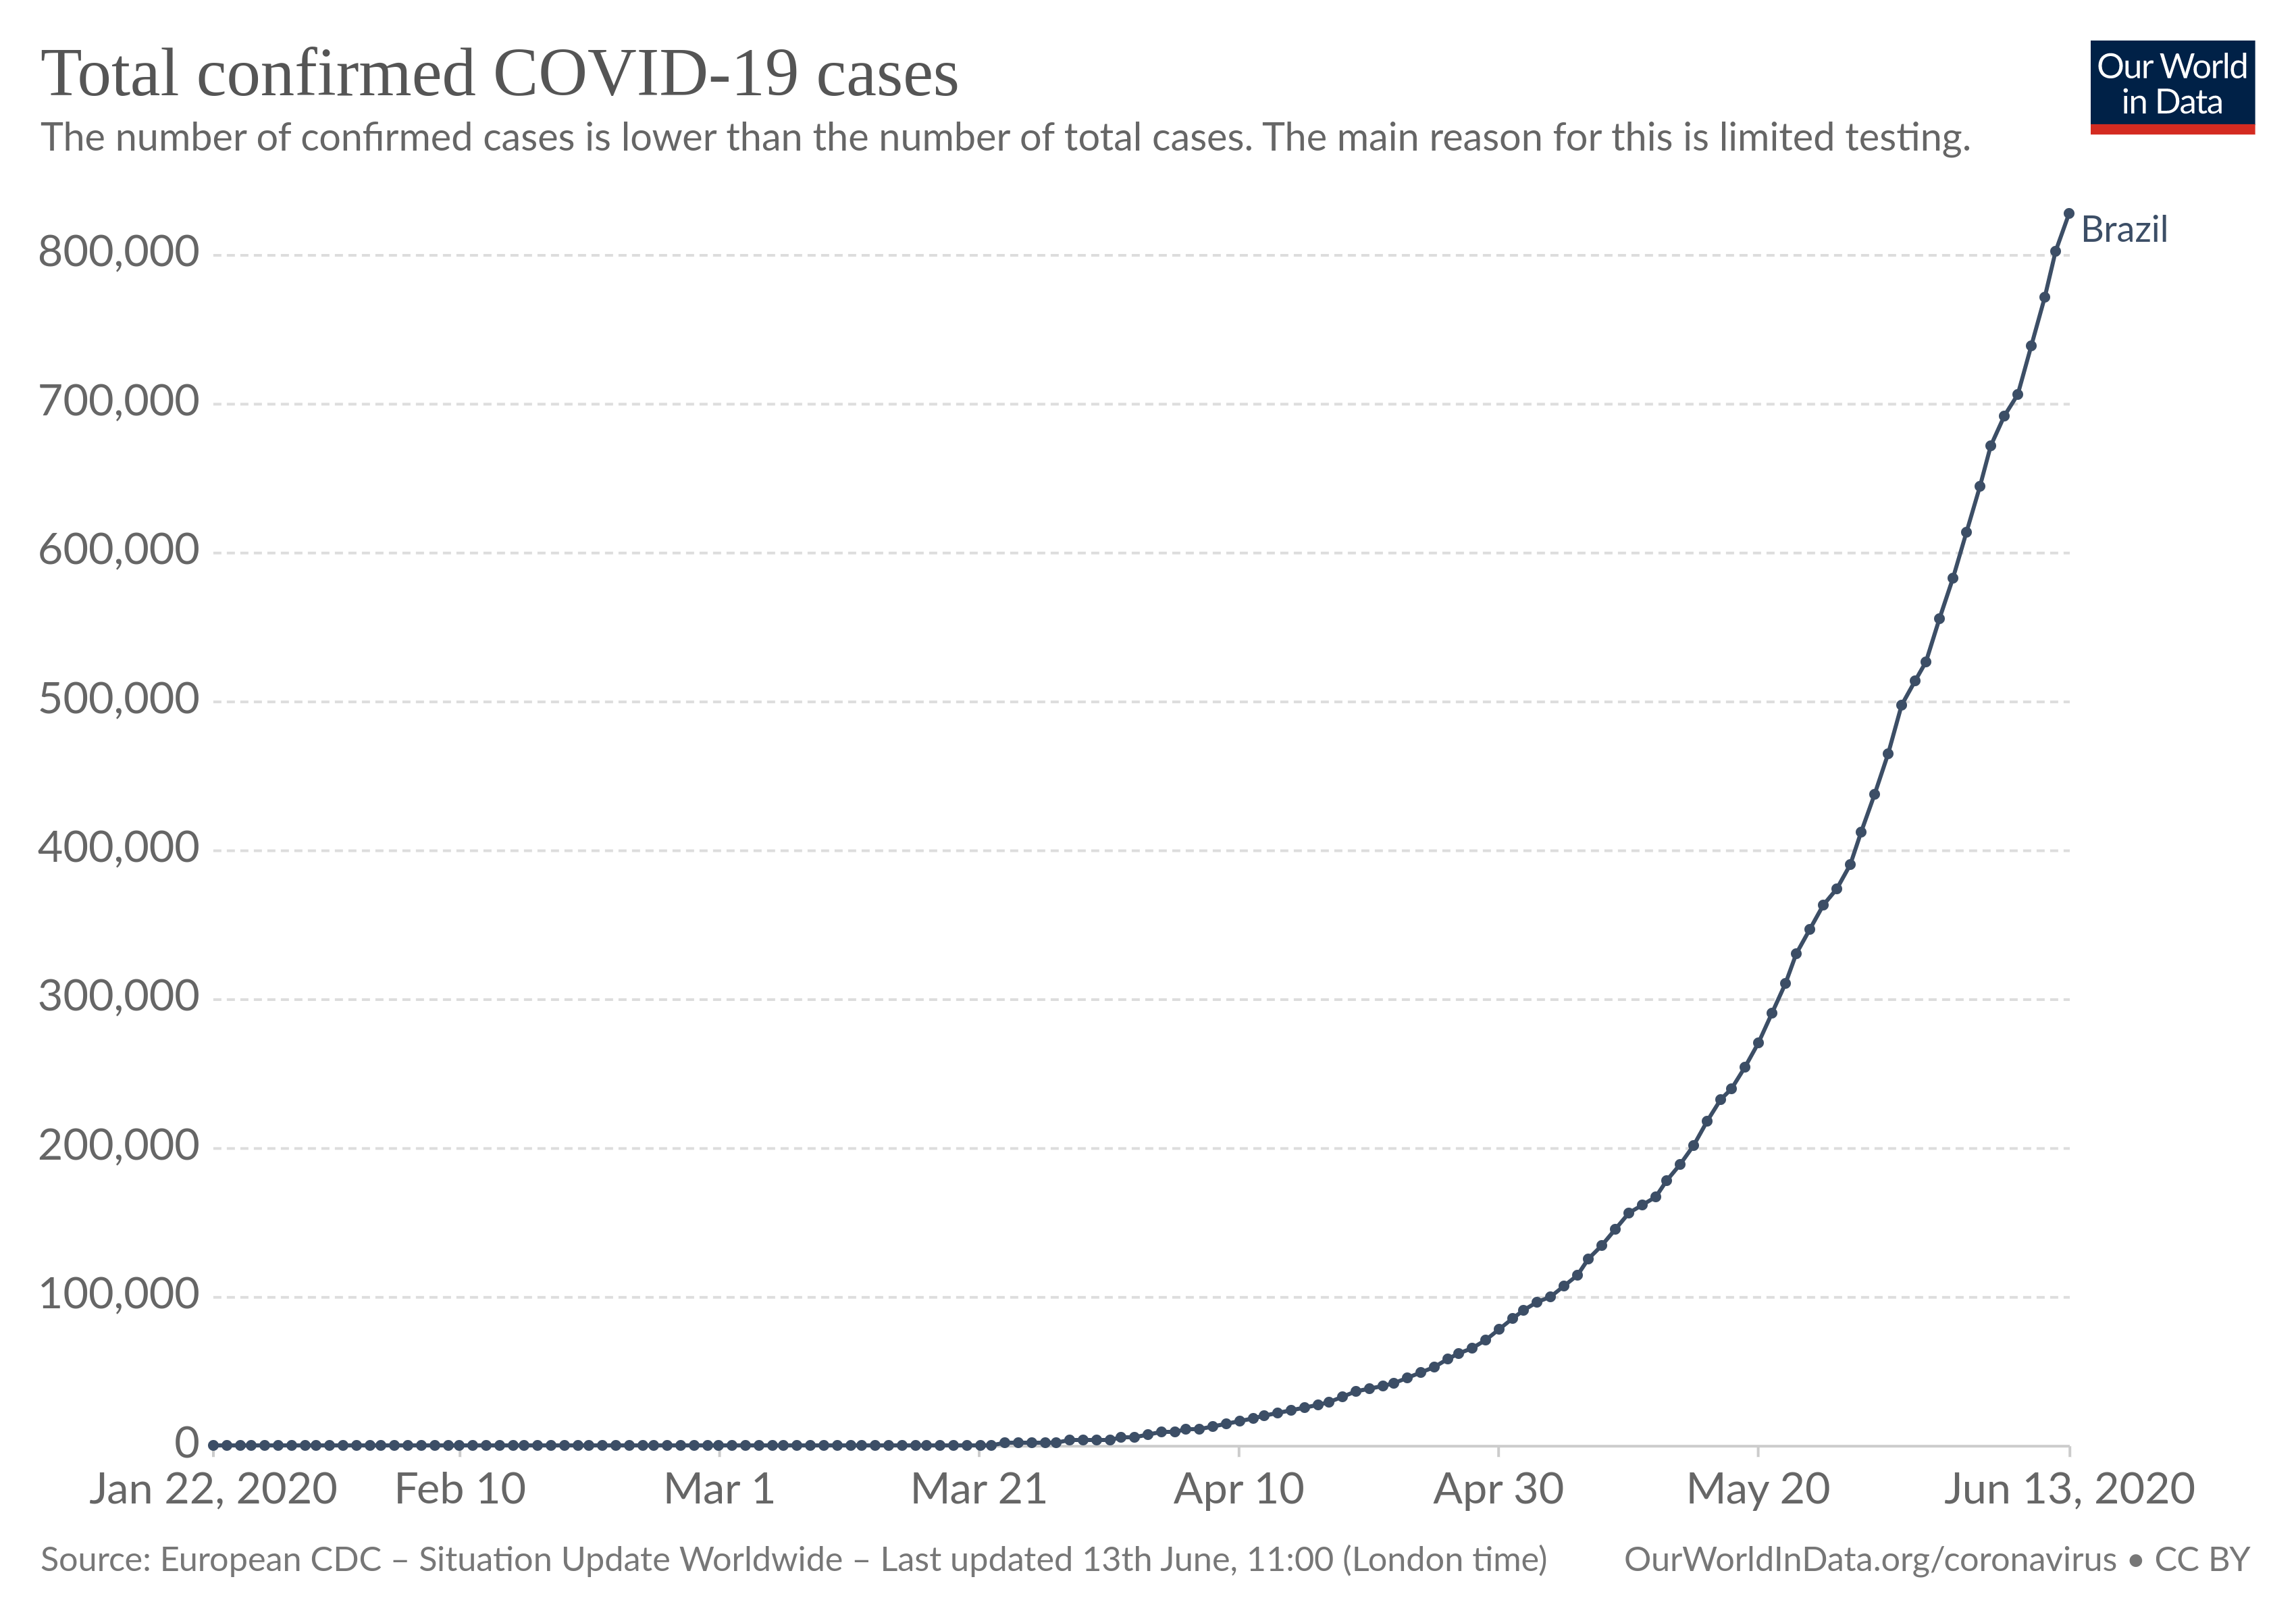
\includegraphics[width=0.7\linewidth]{Figuras/totalcasescovid19.png}

\textbf{Fonte:} Our World in Data (ourworldindata.org).
\end{center}
O crescimento exponencial pode ser modelado pela equação:
$$
I(t) = a\times (1+b)^t,
$$
onde a constante $a$ representa a quantidade de doentes no momento em que se inicia o acompanhamento. A constante $b$ é a taxa de crescimento por unidade de tempo e depende de vários fatores.

Aplicar o logaritmo nos dois lados de uma equação nos permite resolver diversos problemas envolvendo equações exponenciais, transformando-as em equações lineares graças à propriedade do logaritmo da potência. Contudo, podemos escolher a base do logaritmo, o que nos leva ao mesmo resultado de maneiras distintas. Vamos observar isso no exemplo a seguir.

\begin{example}{Uma doença infecciosa}
Vamos supor que um grupo de $10$ pessoas tenha chegado à cidade de São Paulo portando uma nova doença extremamente infecciosa. Suponha que a taxa de crescimento da doença é de $50\%$ ao dia sem que nenhuma medida contenção seja aplicada. Vamos calcular quantos dias levará para que a doença ultrapasse $2000$ pessoas utilizando logaritmos em bases distintas:

Calculando com base $10$:
\begin{align*} &10 \times 1{,}5^t = 2000\\
\Longrightarrow& t\log 1{,}5 = \log 200\\
\Longrightarrow& t = \frac{\log 200}{\log 1{,}5} = \frac{2{,}301029995664}{0{,}17609125905568} \approx 13{,}0672584658868,
\end{align*}
onde utilizamos como aproximação os valores apresentados por uma calculadora científica.

Calculando com base $1,5$:
\begin{align*} &10 \times 1{,}5^t = 2000\\
\Longrightarrow& t\log_{1{,}5} 1{,}5 = \log_{1{,}5} 200\\
\Longrightarrow& t = \log_{1{,}5} 200 \approx 13{,}067258465887,
\end{align*}
onde utilizamos como aproximação os valores apresentados pela calculadora.

Assim apenas no $14^o$ dia, mais de $2000$ pessoas estariam doentes. 

As duas maneiras de resolver estão corretas e a calculadora mostrou o mesmo resultado para $t$ (o último algarismo está diferente, por que estamos trabalhando com aproximações e não com os números exatos). Não poderia ser diferente, pois estamos encontrando o mesmo $t$. Isso nos indica que
$$
\log_{1{,}5} 200 = \frac{\log 200}{\log 1{,}5}.
$$
\end{example}

\begin{Recomenda}{Resolvendo com bases distintas}
{Sugere-se a que os estudantes desenvolvam a atividade para que experimentem o surgimento da propriedade e reforcem a técnica utilizada na solução do exemplo.}
{1}
\end{Recomenda}

\begin{resposta}{Bases distintas}
{Calculando com base $10$:
\begin{align*} &10 \times 2^t = 2000\\
\Rightarrow& t\log 2 = \log 200\\
\Rightarrow& t = \frac{\log 200}{\log 2}\\
& = \frac{\log 2 + 2}{\log 2}= \frac{2{,}3}{0{,}3} \approx 7{,}\overline{6}.
\end{align*}
Calculando com base $2$:
\begin{align*} &10 \times 2^t = 2000\\
\Rightarrow& t\log_{2} 2 = \log_{2} 200\\
\Rightarrow& t = \log_{2} 200  = 1+2\log_2 10 \approx 7{,}66.
\end{align*}}
{1}
\end{resposta}

\begin{task}{Resolvendo com bases distintas}
Vamos supor que um grupo de $10$ pessoas tenha chegado à cidade de São Paulo portando uma nova variedade de uma doença extremamente infecciosa. Suponha que a taxa de crescimento da doença é de $100\%$ ao dia sem que nenhuma medida contenção seja aplicada. Vamos calcular quantos dias levará para que a doença ultrapasse $2000$ pessoas utilizando logaritmos em base $10$ e em base $2$. Utilize as aproximações $\log 2 = 0{,}3$ e $\log_2 10 = 3{,}33$.
\end{task}

\begin{ObjetivoEsp}{Para refletir}
{\begin{itemize}
\item Compreender a estratégia utilizada na atividade como um método para realizar cálculos.
\item Entender que cálculos com logaritmos em quaisquer bases podem ser realizados a partir do conhecimento dos valores dos logaritmos em uma base determinada.
\end{itemize}}
{1}
\end{ObjetivoEsp}

\clearmargin

\begin{resposta}{Para refletir}
{Espera-se que os estudantes concluam, como no exemplo anterior, que 

$
\log_2 200 = \frac{\log 200}{\log 2}.
$

Recomenda-se que seja ressaltado que essa equação pode ser utilizada para calcular esse logaritmo em base $2$ utilizando apenas logaritmos em base $10$.}
{1}
\end{resposta}

\begin{reflection}
Com base no exemplo e na atividade acima, você conseguiria imaginar (fazer uma hipótese) algum modo de calcular $\log_2 200$ utilizando apenas logaritmos em base $10$?
\end{reflection}



Os cálculos realizados nas atividades acima indicam uma propriedade que é valida em um contexto mais geral: a mudança de base (para logaritmos).

\arrange{Mudança de base}\label{secao_mud_base}

\begin{ObjetivoEsp}{Mudança de base}
{\begin{itemize}
\item Comprovar a propriedade da mudança de base.
\item Aplicar a propriedade da mudança de base em aproximações manuais.
\item Aplicar a propriedade da mudança de base em cálculos com a calculadora.
\end{itemize}}
{1}
\end{ObjetivoEsp}

\begin{Recomenda}{Mudança de base}
{A demonstração do teorema demanda o entendimento do conceito de logaritmo e pode ser uma oportunidade para reforçá-lo.

Em seguida recomenda-se que os estudantes resolvam a atividade "Logaritmos com mudança de base" em sala para operacionalizar e fixar a propriedade. Uma vez que esteja claro o significado do teorema, recomenda-se que seja destacada a utilização desse teorema para a efetuação de cálculos com a calculadora, o que é fundamental para a utilização prática e tem a importância reconhecida pela BNCC, que propõe que os estudantes utilizem tecnologias, como calculadoras e planilhas eletrônicas, desde os anos iniciais do Ensino Fundamental. }
{1}
\end{Recomenda}

\begin{description}
\item[Teorema da mudança de base]\label{teo_mud_base} Dados números reais positivos $a,b$ e $c$, com $a \neq 1$, temos que
$$
\log_c b = \frac{\log_a b}{\log_a c}.
$$
\end{description}
\begin{proof}
O logaritmo de $b$ em base $c$ é, por definição, o expoente ao qual devemos elevar $c$ para obter $b$. Assim, basta mostrarmos que $c^{\log_a b/\log_a c} =b$, o que pode calculado lembrando que $a^{\log_a c}=c$:
\begin{align*}
c^{\log_a b/\log_a c} = (a^{\log_a c})^{\log_a b/\log_a c} =a^{\log_a c\log_a b/\log_a c} =  a^{\log_a b} = b,
\end{align*}
onde utilizamos a propriedade da exponencial que $(a^x)^{y/x} = a^{xy/x}$.
\end{proof}

\begin{resposta}{Logaritmos com mudança de base}
{\begin{enumerate}
\item  $\log_3 7=\frac{\log 7}{\log 3} = \frac{0{,}845}{0{,}477} \approx 1{,}7715;$
\item  $\log_7 21=\frac{\log 3 + \log 7}{\log 7} = \frac{0{,}477 + 0{,}845}{0{,}845} \approx 1{,}5645;$
\item  $\log_9 16=\frac{\log 16}{\log 9} =\frac{4\log 2}{2\log 3} = \frac{2*0{,}301}{0{,}477} \approx 1{,}262.$
\end{enumerate}}
{1}
\end{resposta}


\begin{task}{Logaritmos com mudança de base}
Determine o valor dos logaritmos abaixo, sabendo que $\log 2 = 0{,}301$, $\log 3 = 0{,}477$ e $\log 7 = 0{,}845$:
\begin{enumerate}
\item $\log_3 7$;
\item $\log_7 21$;
\item $\log_9 16$.
\end{enumerate}
\end{task}


\begin{observation}{Com a calculadora}
A propriedade da mudança de base é fundamental para calcularmos logaritmos efetivamente, pois a grande maioria das calculadoras e softwares \textbf{não calcula logaritmos em qualquer base}, mas somente em base $10$ ou base $e$ (que estudaremos posteriormente). Assim, para calcular logaritmos de outras bases com a calculadora, precisamos utilizar o teorema da mudança de base, por exemplo:
$$
\log_3 25 = \frac{\log 25}{\log 3} \approx \frac{1{,}397940008672}{0{,}4771212547197} \approx 2{,}9299470414356
$$
\end{observation}

\begin{resposta}{Com a calculadora}
{\begin{enumerate}
\item $\log_2 375=\frac{\log 375}{\log 2} = \frac{2{,}57403126772}{0{,}47712125471} \approx 5{,}39492056215;$
\item $\log_7 698 =\frac{\log 698}{\log 7} = \frac{2{,}84385542262}{0{,}84509804001} \approx 3{,}36511894238;$
\item $\log_{2{,}71} 166 = \frac{\log 166}{\log 2{,}71} = \frac{2{,}22010808804}{0{,}43296929087} \approx 5{,}12763407205.$
\end{enumerate}}
{1}
\end{resposta}


\begin{task}{Com a calculadora}
Utilize uma calculadora ou aplicativo de celular para calcular:
\begin{enumerate}
\item $\log_2 375$;
\item $\log_7 698$;
\item $\log_{2{,}71} 166$.
\end{enumerate}
\end{task}


\exercise
\begin{resposta}{\ref{fuvest} - (Fuvest)}
 {$$
 x-y= \log_4 7 -\frac{\log_4 7^2}{\log_4 16} = \log_4 7 -2\frac{\log_4 7}{2} =0.
 $$}
 {1}
 \end{resposta}

\begin{resposta}{\ref{calculemudbase} - Calcule}
 {$$
 \log_9 128 = \frac{\log 2^7}{\log 3^2}= \frac{7\log 2}{2\log 3}\approx \frac{7\times 0{,}301}{2\times 0{,}477} \approx 2{,}208
 $$}
 {1}
 \end{resposta}

\begin{resposta}{\ref{montanteaplicado} - Montante aplicado}
 {O montante após o tempo $t$ é dado por $m(t) = 2500\times (1{,}03)^t$, de modo que $(1{,}03)^t = \frac{m(t)}{2500}$ e
\begin{align*}
t &= \log_{1{,}03} \left(\frac{m(t)}{2500}\right)=\log_{1{,}03} \left(\frac{3359,79}{2500}\right)\\
&=\frac{1}{\log {1{,}03}} \log \left(\frac{3359,79}{2500}\right)\approx \frac{\log 1{,}344}{\log {1{,}03}} \approx 10{,}002.
\end{align*}
Como sabemos que o capital ficou aplicado por um número inteiro de meses, tomamos o inteiro mais próximo da resposta obtida, que é $10$. Não espera-se uma resposta exata pois os cálculos, mesmo na calculadora, são aproximações.}
 {0}
 \end{resposta}

\begin{resposta}{\ref{veiculodeprec} - Depreciação de veículo}
 {O valor do veículo, após o tempo $t$ é dado por $v(t) = 40000\times (0{,}8)^t$, de modo que $(0{,}8)^t = \frac{v(t)}{40000}$ e
\begin{align*}
t =& \log_{0{,}8} \left(\frac{v(t)}{40000}\right)=\log_{0{,}8} \left(\frac{25600}{40000}\right)=\frac{\log {0{,}64}}{\log {0{,}8}}=2.
\end{align*}}
 {0}
 \end{resposta}
Assim o proprietário ficou com o veículo por dois anos.

\begin{enumerate}

\item {}\label{fuvest}

\textbf{(Fuvest)} Se $x = \log_4 7$ e $y = \log_{16} 49$, então $x - y$ é igual a:

\item {}\label{calculemudbase}

Utilizando as aproximações $\log_{10} 2 =0{,}301$  e $\log_{10} 3=0{,}477$, calcule o valor de $\log_9 128$.

\item {}\label{montanteaplicado}

Um montante de R$\$ 3.359{,}79$ foi obtido de uma aplicação de R$\$ 2.500{,}00$, que foi aplicada por um determinado número (inteiro) de meses, a uma taxa de juros compostos de $3\%$ ao mês. Não foram efetuados outros depósitos no período. Escreva, usando logaritmos, uma formula que permite calcular o tempo em que esse capital ficou aplicado, em seguida, calcule esse tempo utilizando uma calculadora.

\item {}\label{veiculodeprec}

Um veículo que foi adquirido por R$\$ 40.000{,}00$ sofre taxa de depreciação de $20\%$ ao ano. Depois de um determinado tempo o dono quis vender o carro e verificou que depois desse tempo o veículo tinha um valor de R$\$25.600,00$. Escreva, usando logaritmos, a fórmula que permite calcular depois de quanto tempo o carro estava sendo vendido, em seguida, calcule esse tempo.
\end{enumerate}

\explore{Função logarítmica}

\begin{ObjetivoEsp}{Função Logarítmica}
{\begin{itemize}
\item Compreender a definição de decibel.
\item Entender o logaritmo como função (a função logarítmica).
\item Resolver questões envolvendo logaritmos e a unidade de decibel.
\item Identificar gráficos de funções logarítmicas em bases e contextos distintos.
\end{itemize}}
{1}
\end{ObjetivoEsp}


A audição é o sentido que nos faz perceber ondas de pressão no ar, chamadas de ondas acústicas. A intensidade sonora dessas ondas mede quanta energia a onda é capaz de transmitir e a unidade frequentemente utilizada é o \textit{watt por metro quadrado} $W/m^2$. Quanto maior a potência, mais alto percebemos o som; mas a nossa percepção do aumento do som depende do som já presente no ambiente. Por exemplo uma pessoa falando em uma sala quieta pode parecer bastante alto, enquanto a mesma pessoa falando em um show de rock não faz diferença alguma.

\begin{Recomenda}{Função Logarítmica}
{A habilidade EM13MAT305 traz contextos nos quais os logaritmos são utilizados. Um contexto de importância prática e que aparece com certa frequência em concursos é o de ondas sonoras. Essa exploração é realizada para introduzir a função logarítmica, uma vez que existem ondas sonoras de todo nível de intensidade, de modo a dar espaço para os contextos e raciocínios pré-formais antes da introdução do conteúdo per si, no espírito da Educação Matemática Realística.}
{1}
\end{Recomenda}

Para lidarmos com o modo como percebemos o som e a potência das ondas sonoras, utilizamos uma unidade chamada de \textbf{decibel (dB)} que mede o \textit{nível sonoro} dos sons em relação a o limiar da audição humana. Observe a Tabela \ref{tab_decibeis} com diferentes sons, seus níveis sonoros em decibéis, suas intensidades sonoras em $W/m^2$ e percepções ao ouvido humano
\begin{table}[!ht]
\centering
\caption{Níveis sonoros e intensidades sonoras.}\label{tab_decibeis}
\begin{tabular}{lcrl}
\textbf{Fonte do som} & \textbf{Nível} & \textbf{Intensidade} & \textbf{Percepção}\\
 & \textbf{(dB)} & \textbf{$W/m^2$} & \\
\hline \hline Arma de fogo próxima ao ouvido & $130$ & $10$ & Dor\\
Avião decolando & $120$ & $1$ & Desconforto\\
Perfuratriz pneumática & $110$ & $10^{-1}$ & Muito alto\\
Sirene & $100$ & $10^{-2}$ & \\
Buzina alta & $90$ & $10^{-3}$ & Alto\\
Porta batendo & $80$ & $10^{-4}$ & \\
Rua com tráfego pesado & $70$ & $10^{-5}$ & Barulhento\\
Conversa animada & $60$ & $10^{-6}$ & \\
Conversa normal & $50$ & $10^{-6}$ & Moderado\\
Rádio volume baixo & $40$ & $10^{-8}$ & Quieto\\
Noite tranquila no campo & $30$ & $10^{-9}$ & \\
Sala quieta & $20$ & $10^{-10}$ & Muito quieto\\
Sussurrar da folhas & $10$ & $10^{-11}$ & \\
Limiar da audição & $0$ & $10^{-12}$ & 
\end{tabular}\\
{\textbf{Fonte:} Adaptado de um artigo de EEWeb.com por Andrew Carter}
\end{table}

\begin{resposta}{Para refletir}
{A potência é multiplicada por $10$, enquanto soma-se $10$ ao nível de intensidade. Isso significa que a potência cresce exponencialmente, enquanto o nível de intensidade cresce linearmente.}
{1}
\end{resposta}

\begin{reflection}
A percepção da altura de um som é subjetiva e depende da distância da fonte emissora, que não está escrita na tabela. Levando isso em consideração, você concorda com as percepções da coluna da direita?\\
Notamos que o nível sonoro (em dB) aumenta de 10 em 10 para os valores tabelados. E a intensidade sonora, como ela varia entre os diferentes níveis? 
\end{reflection}

A intensidade sonora é multiplicada por $10$ quando soma-se $10$ ao nível sonoro. Isso quer dizer que o decibel mede quantas ordens de magnitude a intensidade do som está em relação ao limiar da audição humana e multiplica o número de ordens de magnitude por $10$. Isso apreende o fato de ser necessária uma mudança drástica na intensidade para \textit{percebermos}  uma mudança no nível do som. Por exemplo uma pessoa falando à altura de $50db$ em um show de rock à altura $110db$ não muda a percepção de barulho.

\begin{observation}{O decibel (dB)}
O \textbf{decibel (dB)} é uma unidade logarítmica utilizada para medir o nível sonoro. Toma-se como referência o menor som audível ao ouvido humano $I_0$ (que é considerado com intensidade sonora de $10^{-12}\, watts/m^2$) e o decibel indica quantas ordens de grandeza uma onda sonora tem em relação à onda de referência através da expressão:
$$
I_{dB} = 10 \log_{10} \left(\frac{I}{I_0}\right),
$$
onde $I$ é a intensidade acústica, medida em watts por metro quadrado. Utilizando a propriedade do logaritmo do quociente vemos que o nível sonoro pode ser calculado, equivalentemente, por
$$
I_{dB} = 120 + 10 \log_{10} I.
$$
\end{observation}



\begin{task}{Fogos de Artifício}
Algumas cidades brasileiras estão limitando o nível sonoro dos fogos de artifício utilizados em celebrações, permitindo apenas fogos de até $100dB$ a 100 metros de distância. A classificação do som como forte ou fraco está relacionada à intensidade sonora, medida em watts por metro quadrado $W/m^2$. A menor intensidade sonora audível ou limiar de audibilidade possui intensidade $I_0 = 10^{-12} W/m^2$. O nível sonoro pode ser calculado a partir da intensidade da onda pela expressão $I_{dB} = 10 \times log(I/I_0)$, onde $I_0$ é o limiar de audibilidade. Um técnico mede a intensidade sonora de um foguete como sendo de $3{,}7 W/m^2$ a 100 metros de distância. Esse foguete poderia ser utilizado de acordo com a norma determinada por essas cidades?
\end{task}


\begin{Recomenda}{Fogos de Artifício}
{Recomenda-se a resolução da atividade em sala para oportunizar o surgimento de dúvidas, tendo em vista que a definição de decibel pode parecer complicada à primeira vista.}
{1}
\end{Recomenda}



\begin{resposta}{Fogos de Artifício}
{Calculamos o nível de intensidade
\begin{align*}
I_{dB} =& 10 \log \left(\frac{3{,}7}{10^{-12}}\right)\\
=& 10 \log (3{,}7\times 10^{12})\\
=& 10 (\log 3{,}7+12)\\
=& 10\times 12{,}5682 = 125{,}682
\end{align*}
e verificamos que o artefato estaria em desacordo com a norma.}
{0}
\end{resposta}


\arrange{Função logarítmica}

\begin{Recomenda}{Função Logarítmica}
{Recomenda-se ressaltar que são possíveis ondas sonoras das mais diversas intensidades sonoras, de modo que devemos pensar no nível sonoro como uma uma função da intensidade. Essa função associa a cada intensidade sonora, que é sempre um número positivo, o respectivo nível sonoro em decibéis.

Dessa maneira maneira temos uma função logarítmica, contudo cabe ressaltar que a definição de função logarítmica apresentada (e que é, provavelmente, a mais frequente) não apresenta uma constante multiplicando-a ou uma constante dividindo o argumento, como no exemplo apresentado.}
{1}
\end{Recomenda}

Os sons na natureza podem ter os mais diversos valores, e não estarem definidos apenas para intensidades $I = 10^n$, para algum valor $n \in \mathbb{Z}$, como na Tabela \ref{tab_decibeis}. Assim o nível sonoro, em decibéis, é uma \textit{função} da intensidade sonora ($I$) do som:
$$
I_{dB}(I) = 10 \log_{10} \left(\frac{I}{10^{-12}}\right).
$$

Esse é um exemplo de uma função logarítmica!

\begin{description}
\item[Definição]\label{teo_mud_base}
Dado um número real positivo $a$, $a \neq 1$, chama-se \textbf{função logarítmica de base} $a$ à função $f: \mathbb{R}_+^* \to \mathbb{R}$ definida pela lei
$$
f(x) = \log_a x.
$$
\end{description}

\begin{observation}{A função calcula o logaritmo dos números reais positivos}
Ou seja, a função logarítmica de base $a$ é aquela que associa a cada número real positivo o logaritmo daquele número.
\end{observation}

\begin{ObjetivoEsp}{Gráficos dos logaritmos}
{Reconhecer gráficos das funções logarítmicas de bases maior do que $1$ e menor do que $1$.

Relacionar os gráficos de funções logarítmicas de base $a>1$ e $1/a$.}
{1}
\end{ObjetivoEsp}

\begin{Recomenda}{Gráficos dos logaritmos}
{O enunciado apresenta os valores dos logaritmos para encurtar o tempo da atividade, tendo em vista que cálculos de logaritmos já foram explorados nas atividades anteriores. Recomenda-se a reflexão sobre os valores do logaritmo de base $1/2$, se necessário com mediação do/a  professor/a, para que se conclua que eles são iguais a "menos"\, os valores listados. Como mediação pode-se comparar $2^3=8$, $2^{-3}=1/8$, $1/2^3=1/8$ e $(1/2)^{-3}=8$.}
{1}
\end{Recomenda}

\begin{task}{Gráficos dos logaritmos}
Utilize as aproximações abaixo, com dois dígitos de precisão, dos logaritmos em base $2$ para esboçar o gráfico de $f(x) = \log_{2} x$ no espaço quadriculado abaixo.
\begin{align*}
& \log_{2} 1/8 = -3; \,\, \log_{2} 1/4 = -2; \,\, \log_{2} 1/2 = -1; \,\, \log_{2} 1 = 0; \,\, \log_{2} 2  = 1; \,\, \log_{2} 3  =  1{,}58; \,\,\\
& \log_{2} 4  = 2; \,\, \log_{2} 5 = 2{,}32; \,\, \log_{10} 1 = 0; \,\, \log_{2} 6 = 2{,}58; \,\, \log_{2} 7  = 2{,}8; \,\, \log_{2} 8  = 3; \,\,\\
& \log_{2} 9  = 3{,}16; \,\, \log_{2} 10  = 3{,}32.
\end{align*}
Após esboçar esse gráfico, converse com seus colegas e com o professor como utilizar esses valores para esboçar o gráfico $g(x) = \log_{1/2} x$ e tente traçá-lo.
\end{task}



\begin{resposta}{Gráficos dos logaritmos}
{Os gráficos de $f$ em verde e $g$ em laranja.

\begin{center}
\resizebox{0.7\marginparwidth}{!}{
\begin{tikzpicture}
\foreach \n in {0,...,10}{% 10 (instead of 9) is used here to make sure the last line is drawn.
            \draw[gray] (\n,0) -- (\n,10);
            \draw[gray] (0,\n) -- (10,\n);
%            \node at (\n-0.2, 3.7) {\n};
}
\foreach \n in {-4,...,6}{\node at (-0.2, \n+3.7) {\n};}
\draw[black,->] (0,-0.3) -- (0,10.3);
%\node[black] at (-0.2,10.3) {y};
\draw[black,->] (-0.3,4.0) -- (10.3,4.0);
%\node[black] at (10.3,3.7) {x};
\draw[penaqua, domain=0.125:10] plot (\x, {4+log2(\x)});
\draw[penlaranja, domain=0.125:10] plot (\x, {4-log2(\x)});
\end{tikzpicture}}\end{center}}
{0}
\end{resposta}

\begin{center}
\resizebox{\linewidth}{!}{
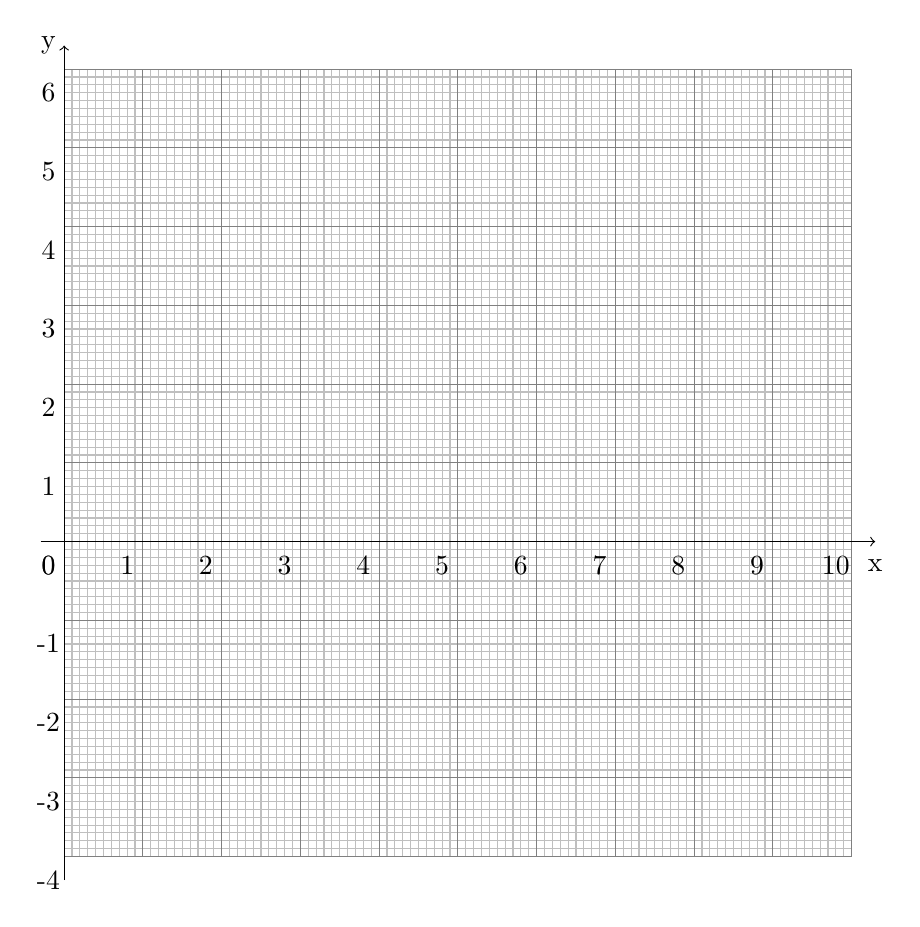
\begin{tikzpicture}
\foreach \i in {0,...,100}{% 10 (instead of 9) is used here to make sure the last line is drawn.
            \draw[lightgray] (0.1*\i,0) -- (0.1*\i,10);
            \draw[lightgray] (0,0.1*\i) -- (10,0.1*\i);}
\foreach \n in {0,...,10}{% 10 (instead of 9) is used here to make sure the last line is drawn.
            \draw[gray] (\n,0) -- (\n,10);
            \draw[gray] (0,\n) -- (10,\n);
            \node at (\n-0.2, 3.7) {\n};}
\foreach \n in {-4,...,6}{\node at (-0.2, \n+3.7) {\n};}
\draw[black,->] (0,-0.3) -- (0,10.3);
\node[black] at (-0.2,10.3) {y};
\draw[black,->] (-0.3,4.0) -- (10.3,4.0);
\node[black] at (10.3,3.7) {x};
\end{tikzpicture}}
\end{center}

\begin{ObjetivoEsp}{Invertendo a base}
{Comprovar a propriedade da inversão da base para logaritmos.}
{1}
\end{ObjetivoEsp}

\begin{observation}{Invertendo a base}
A atividade \textit{Gráficos dos logaritmos} pode ser realizada se percebermos que $\log_{1/2} x = -\log_{2} x$. Essa propriedade é uma consequência do teorema da mudança de base:
$$
\log_{1/a} x = \frac{\log_a x}{\log_a {1/a}} = \frac{\log_a x}{-1} = -\log_a x. 
$$
\end{observation}

\begin{ObjetivoEsp}{Para refletir}
{Compreender para que valores faz sentido calcular o logaritmo e concluir que o domínio da função logarítmica contém apenas os números reais positivos.}
{1}
\end{ObjetivoEsp}

\begin{Recomenda}{Para refletir}
{Uma vez introduzida a função logarítmica e seu gráfico, surge naturalmente o questionamento: o que ocorre com o gráfico para $x$ negativo? Pode-se utilizar esse questionamento para reforçar que o argumento do logaritmo não pode ser negativo. Para justificar esse fato pode-se ressaltar que o logaritmo é o expoente em que a base deve ser elevada para a obtenção do argumento (logaritmando) e que as exponenciais só geram valores positivos (mesmo com expoentes negativos).

Essa atividade pode levar os estudantes a questionar o sinal da base do logaritmo e pode ser uma oportunidade para explorar esse ponto. Nesse caso também pode ser necessário retornar à definição da função exponencial $f(x)=a^x$, que só faz sentido para todo $x \in \mathbb{R}$ se $a>0$, apesar de fazer sentido para $x \in \mathbb{Z}$.

Por fim relembramos que a exploração desse tipo de questão é indicada pela BNCC, por exemplo na EM13MAT403.}
{1}
\end{Recomenda}


\begin{reflection}{O domínio contém apenas o semieixo positivo!}
Por que calculamos apenas os logaritmos de números reais positivos? Qual seria o problema para calcular $\log_2 (-4)$?
\end{reflection}

\begin{resposta}{Para refletir}
{Encontrar o valor de $\log_2 (-4)$ é o mesmo que encontrar o expoente ao qual devemos elevar $2$ para obter $-4$. Agora $2^x>0$ para qualquer $x \in \mathbb{R}$, de modo que não existe número real $x$ de modo que $2^x=-4$. O mesmo raciocínio vale para qualquer outro logaritmando negativo. Por isso só faz sentido calcular o logaritmo de números (logaritmandos) positivos e o domínio das funções logarítmicas só pode conter os números reais positivos.}
{1}
\end{resposta}



\begin{task}{Comparando funções conhecidas}
As curvas na figura representam as funções $f(x) = 2x-3$, $g(x)=2x^2-1$, $h(x)=1{,}5^x$ e $l(x)=\log_2 x$. Identifique que curva representa cada função. Calcular o valor da função para alguns valores de $x$ pode auxiliar na identificação.

\begin{center}
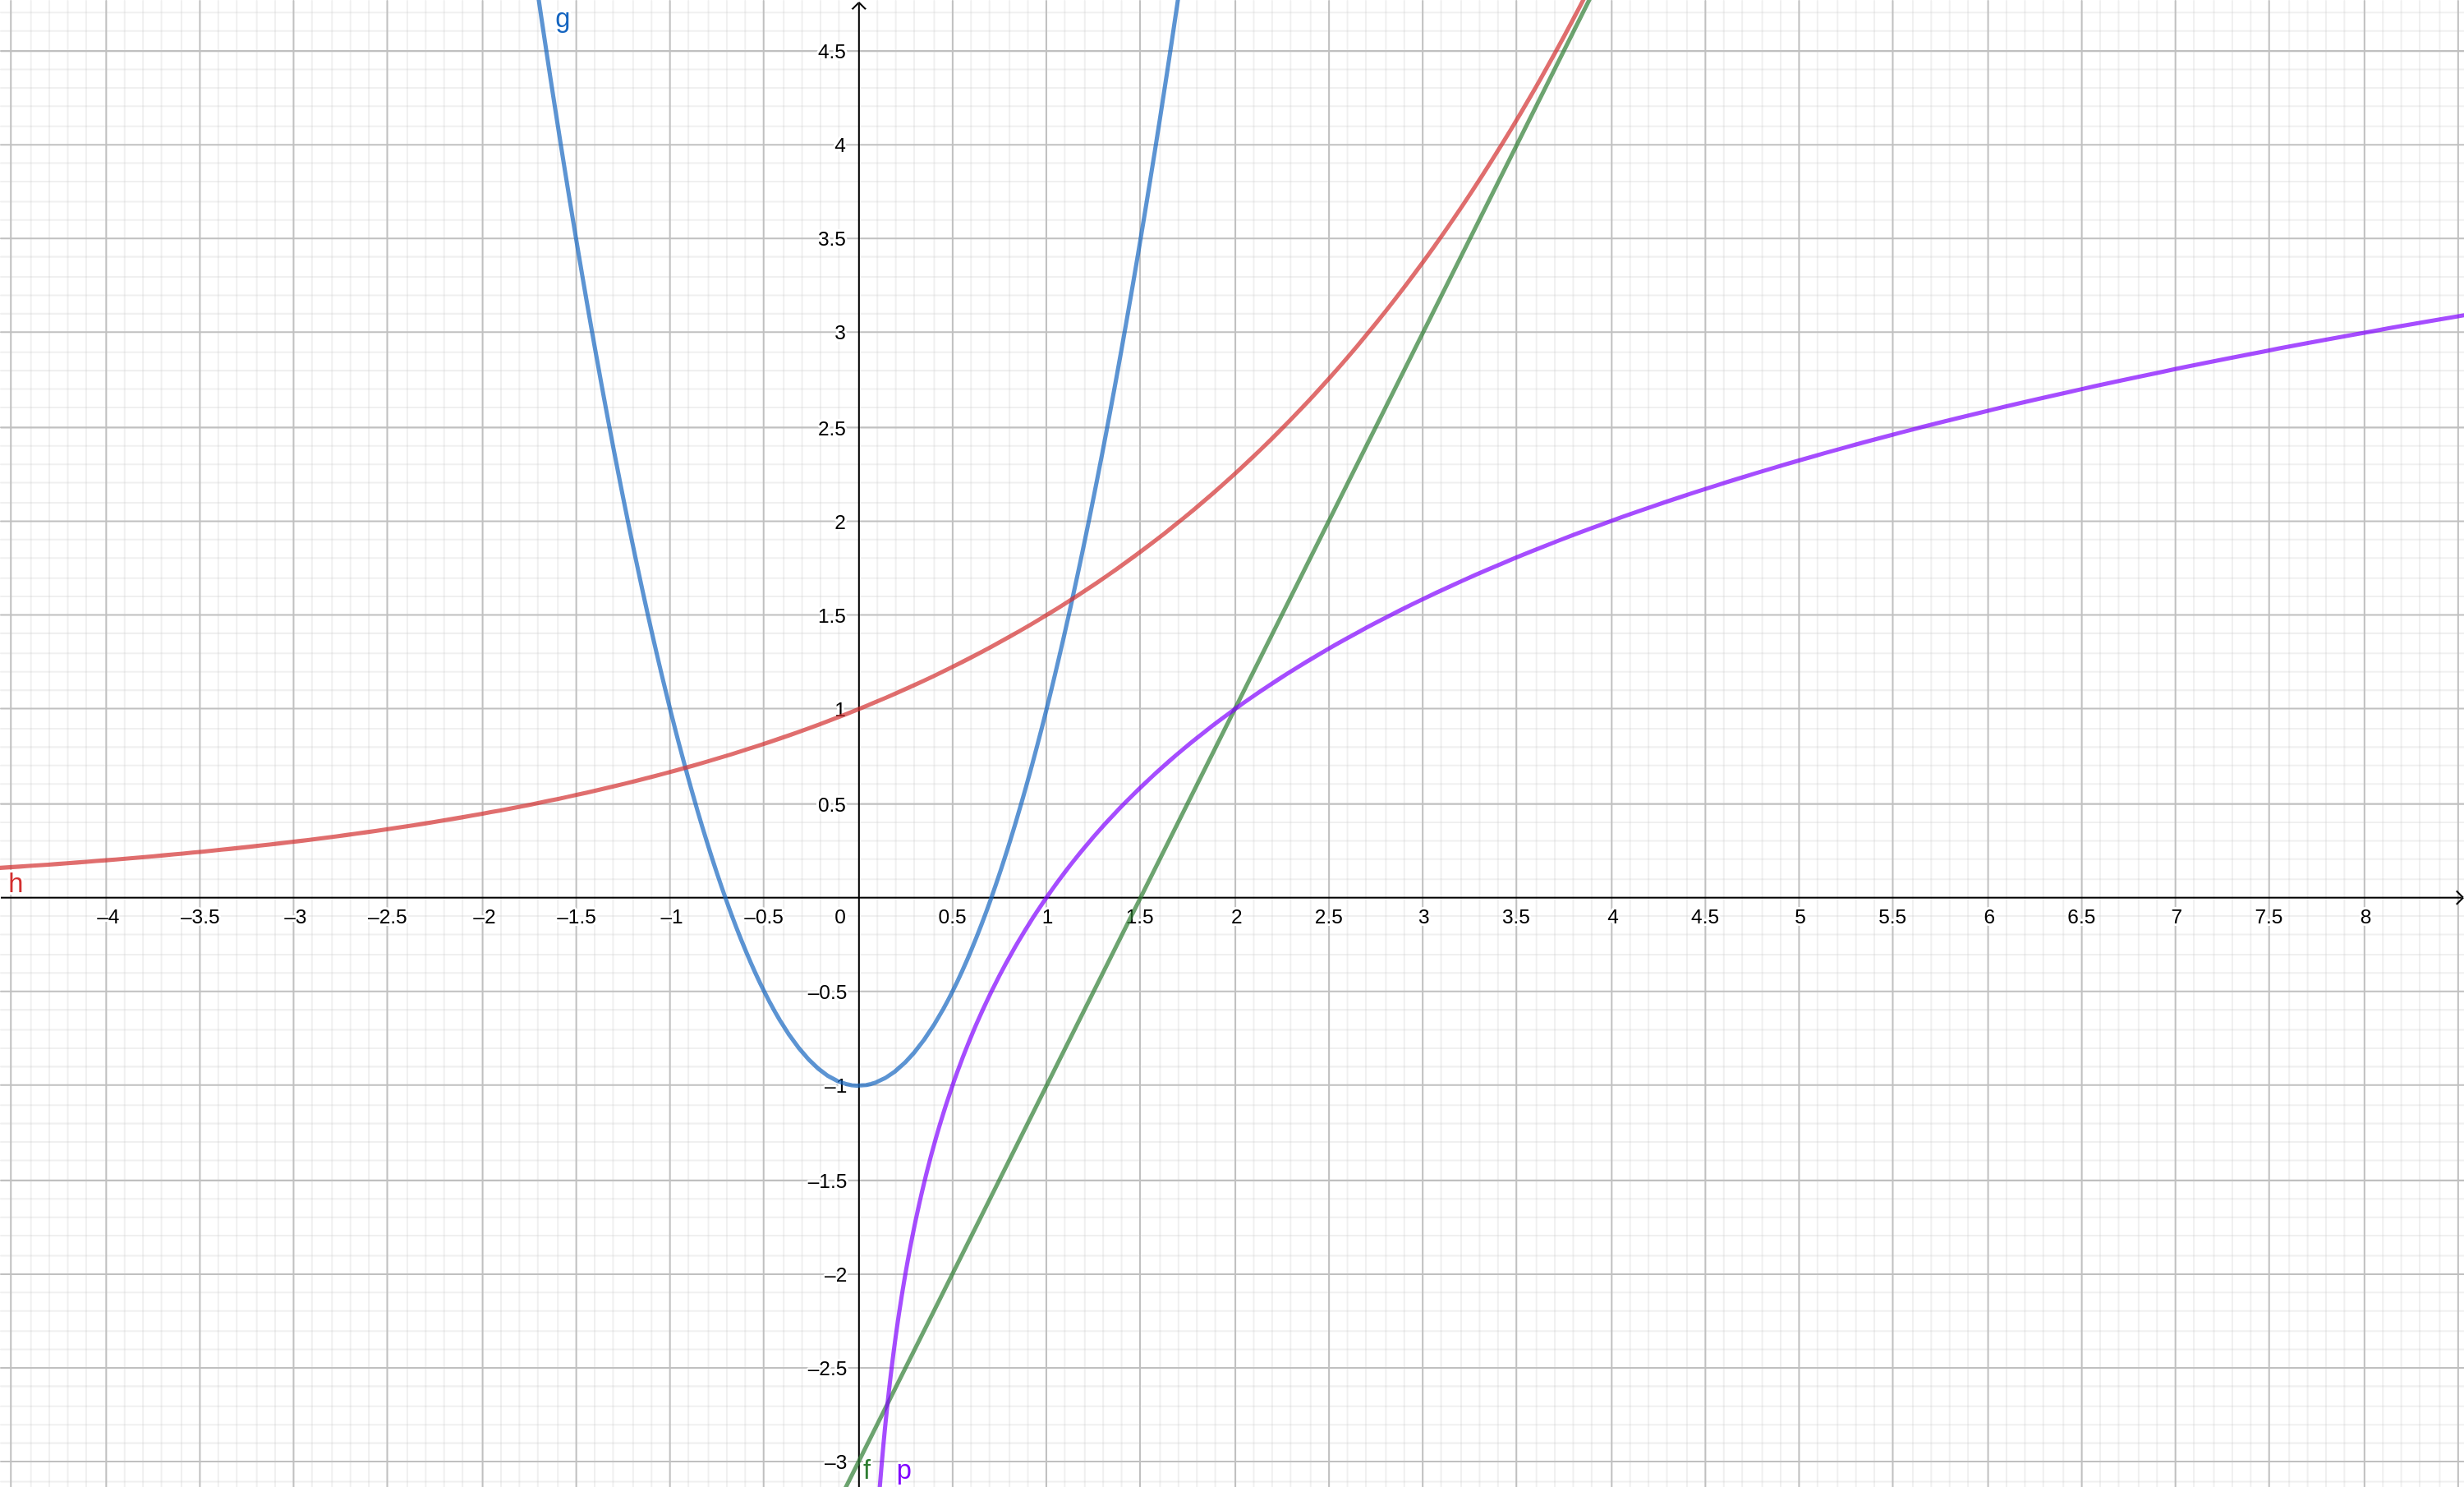
\includegraphics[width=0.8\linewidth]{Figuras/graficos_varias_funcoes}
\end{center}
\end{task}

\begin{ObjetivoEsp}{Comparando funções}
{Reconhecer o gráfico de uma função logarítmica e diferenciá-la de outras funções conhecidas.}
{1}
\end{ObjetivoEsp}

\begin{Recomenda}{Comparando funções conhecidas}
{A atividade \textit{"Comparando funções conhecidas"} compara o gráfico da função logarítmica com os gráficos de outras funções conhecidas. Essa comparação ajuda a distinguir a função recém apresentada das demais e serve de preparação para as aplicações práticas a seguir, que demandam o conhecimento do perfil da função.}
{1}
\end{Recomenda}

\begin{resposta}{Comparando funções conhecidas}
{$f(x)$ descreve uma reta e foi plotada em verde, $g(x)$ descreve uma parábola e foi plotada em azul, $h(x)$ descreve uma exponencial, cujos valores são sempre positivos, e foi plotada em vermelho e $l(x)$ é uma função logarítmica, definida apenas no semi-eixo positivo, e foi plotada em roxo.}
{1}
\end{resposta}


\begin{ObjetivoEsp}{Crescimento logarítmico...}
{Reconhecer que dados reais podem ser aproximados por funções conhecidas.}
{1}
\end{ObjetivoEsp}

\begin{Recomenda}{Crescimento logarítmico...}
{Recomenda-se, a seguir, a exploração do exemplo com dados do número de mortes confirmadas da Covid-19 na França. O exemplo mostra como os gráficos de funções conhecidas podem ser utilizadas para identificar tendências, auxiliando na análise de situações concretas, que contribui na tomada de decisão, auxiliando no desenvolvimento da habilidade EM13MAT101, indicada na BNCC.}
{1}
\end{Recomenda}

\begin{example}{Crescimento logarítmico e exponencial}
A figura abaixo mostra o total de mortes confirmadas causadas pela Covid-19 na França a cada dia, entre 15 de fevereiro e 13 de junho. Observamos no gráfico uma mudança no padrão da curva por volta da data de 7 de abril. No período inicial a curva é melhor aproximada por uma exponencial e depois é melhor aproximada por uma função logarítmica.
\begin{center}
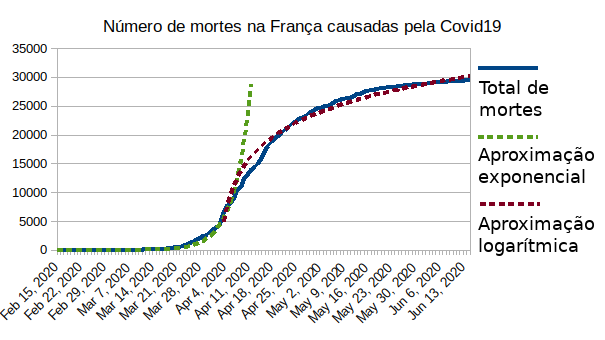
\includegraphics[width=0.95\linewidth]{Figuras/mortes_franca}

\textbf{Fonte:} dados do site \textit{Our World in Data} (ourworldindata.org).
\end{center}

Buscar uma função que melhor aproxime os dados de um determinado experimento ou acontecimento da vida real é um procedimento, chamado \textit{ajuste de curvas}, muito utilizado em todas as áreas da ciência. Os ajustes de curvas podem ser utilizados para prever tendências em dados futuros e permitir que sejam tomadas medidas preventivas.

A curva exponencial sugere que haveria um crescimento muito rápido no número de mortes. Contudo a redução posterior mostra um número muito menor, que pode ter sido causada pelas medidas adotadas pelo governo Francês (entre outras possibilidades).
\end{example}

\begin{ObjetivoEsp}{Brasil e Reino Unido}
{\begin{itemize}
\item Utilizar o ajuste de curvas para identificar tendências em dados reais.
\item Interpretar criticamente a situação dos dois países na pandemia de Covid-19 pela análise dos gráficos das funções representadas e das taxas de variação, com ou sem apoio de tecnologias digitais. (EM13MAT101)
\item Analisar tabelas, gráficos e amostras de pesquisas estatísticas apresentadas em relatórios divulgados por diferentes meios de comunicação, identificando, quando for o caso, inadequações que possam induzir a erros de interpretação, como escalas e amostras não apropriadas. (EM13MAT102)
\end{itemize}}
{1}
\end{ObjetivoEsp}

\begin{Recomenda}{Brasil e Reino Unido}
{A atividade propõem a análise de tendências nos gráficos apresentados comparando as situações do Brasil e do Reino Unido. O resultado esperado da atividade não é uma resposta exata, mas uma discussão sobre o tema, que pode ser realizada em grupo na sala de aula. Espera-se que os alunos identifiquem uma mudança na tendência do gráfico do Reino Unido, de crescimento exponencial (muito rápido) para logarítmico (mais lento) um pouco depois do dia 10 de abril, enquanto que no Brasil o número de mortos parece estar abandonando o crescimento exponencial somente em 13 de junho. O número de mortos no Brasil, no momento da aparente mudança no perfil, está entre 3x e 4x o número de mortos no Reino Unido no momento de mudança. Isso poderia sugerir que o Brasil atingiria entre 3x e 4x o número de mortos, se a pandemia continuasse se  desenvolvendo da mesma forma nos dois países e o perfil final dos dois países fosse parecido (o que não sabemos antes do final da pandemia). Recomenda-se que o/a professor/a busque dados atualizados da pandemia e mostre aos estudantes, assim os alunos poderiam verificar se as suas hipóteses e previsões realizadas concretizaram-se.

Ainda na atividade é importante ressaltar em uma análise que há grandes diferenças entre os países e essas contribuem bastante para o resultado final. Essa atividade poderia ser desenvolvida de forma interdisciplinar com a disciplina de geografia, que poderia explorar diferenças demográficas, sociais, dos sistemas de saúde, socio-econômicas e das reações socio-políticas dos países. Por exemplo, citamos o fato óbvio que as populações do Brasil (de 209,5 milhões (2018), segundo o Banco mundial) e do Reino Unido (de 66,65 milhões (2018), segundo o Banco Mundial) são fatores importantes a se levar em consideração.}
{1}
\end{Recomenda}

\begin{task}{Brasil e Reino Unido na Pandemia}
Observando o gráfico abaixo, em que data (aproximadamente) o crescimento mudou de exponencial para logarítmico no Reino Unido? E no Brasil? Apesar do número ser parecido na data final do gráfico, você acredita que o número total de mortos manteve-se próximo? Que fatores sociais, econômicos e demográficos podem ter influenciado o desenvolvimento da pandemia nesses países? 

\begin{center}
\captionof{figure}{Mortes confirmadas Covid-19 no Brasil e no Reino Unido.}
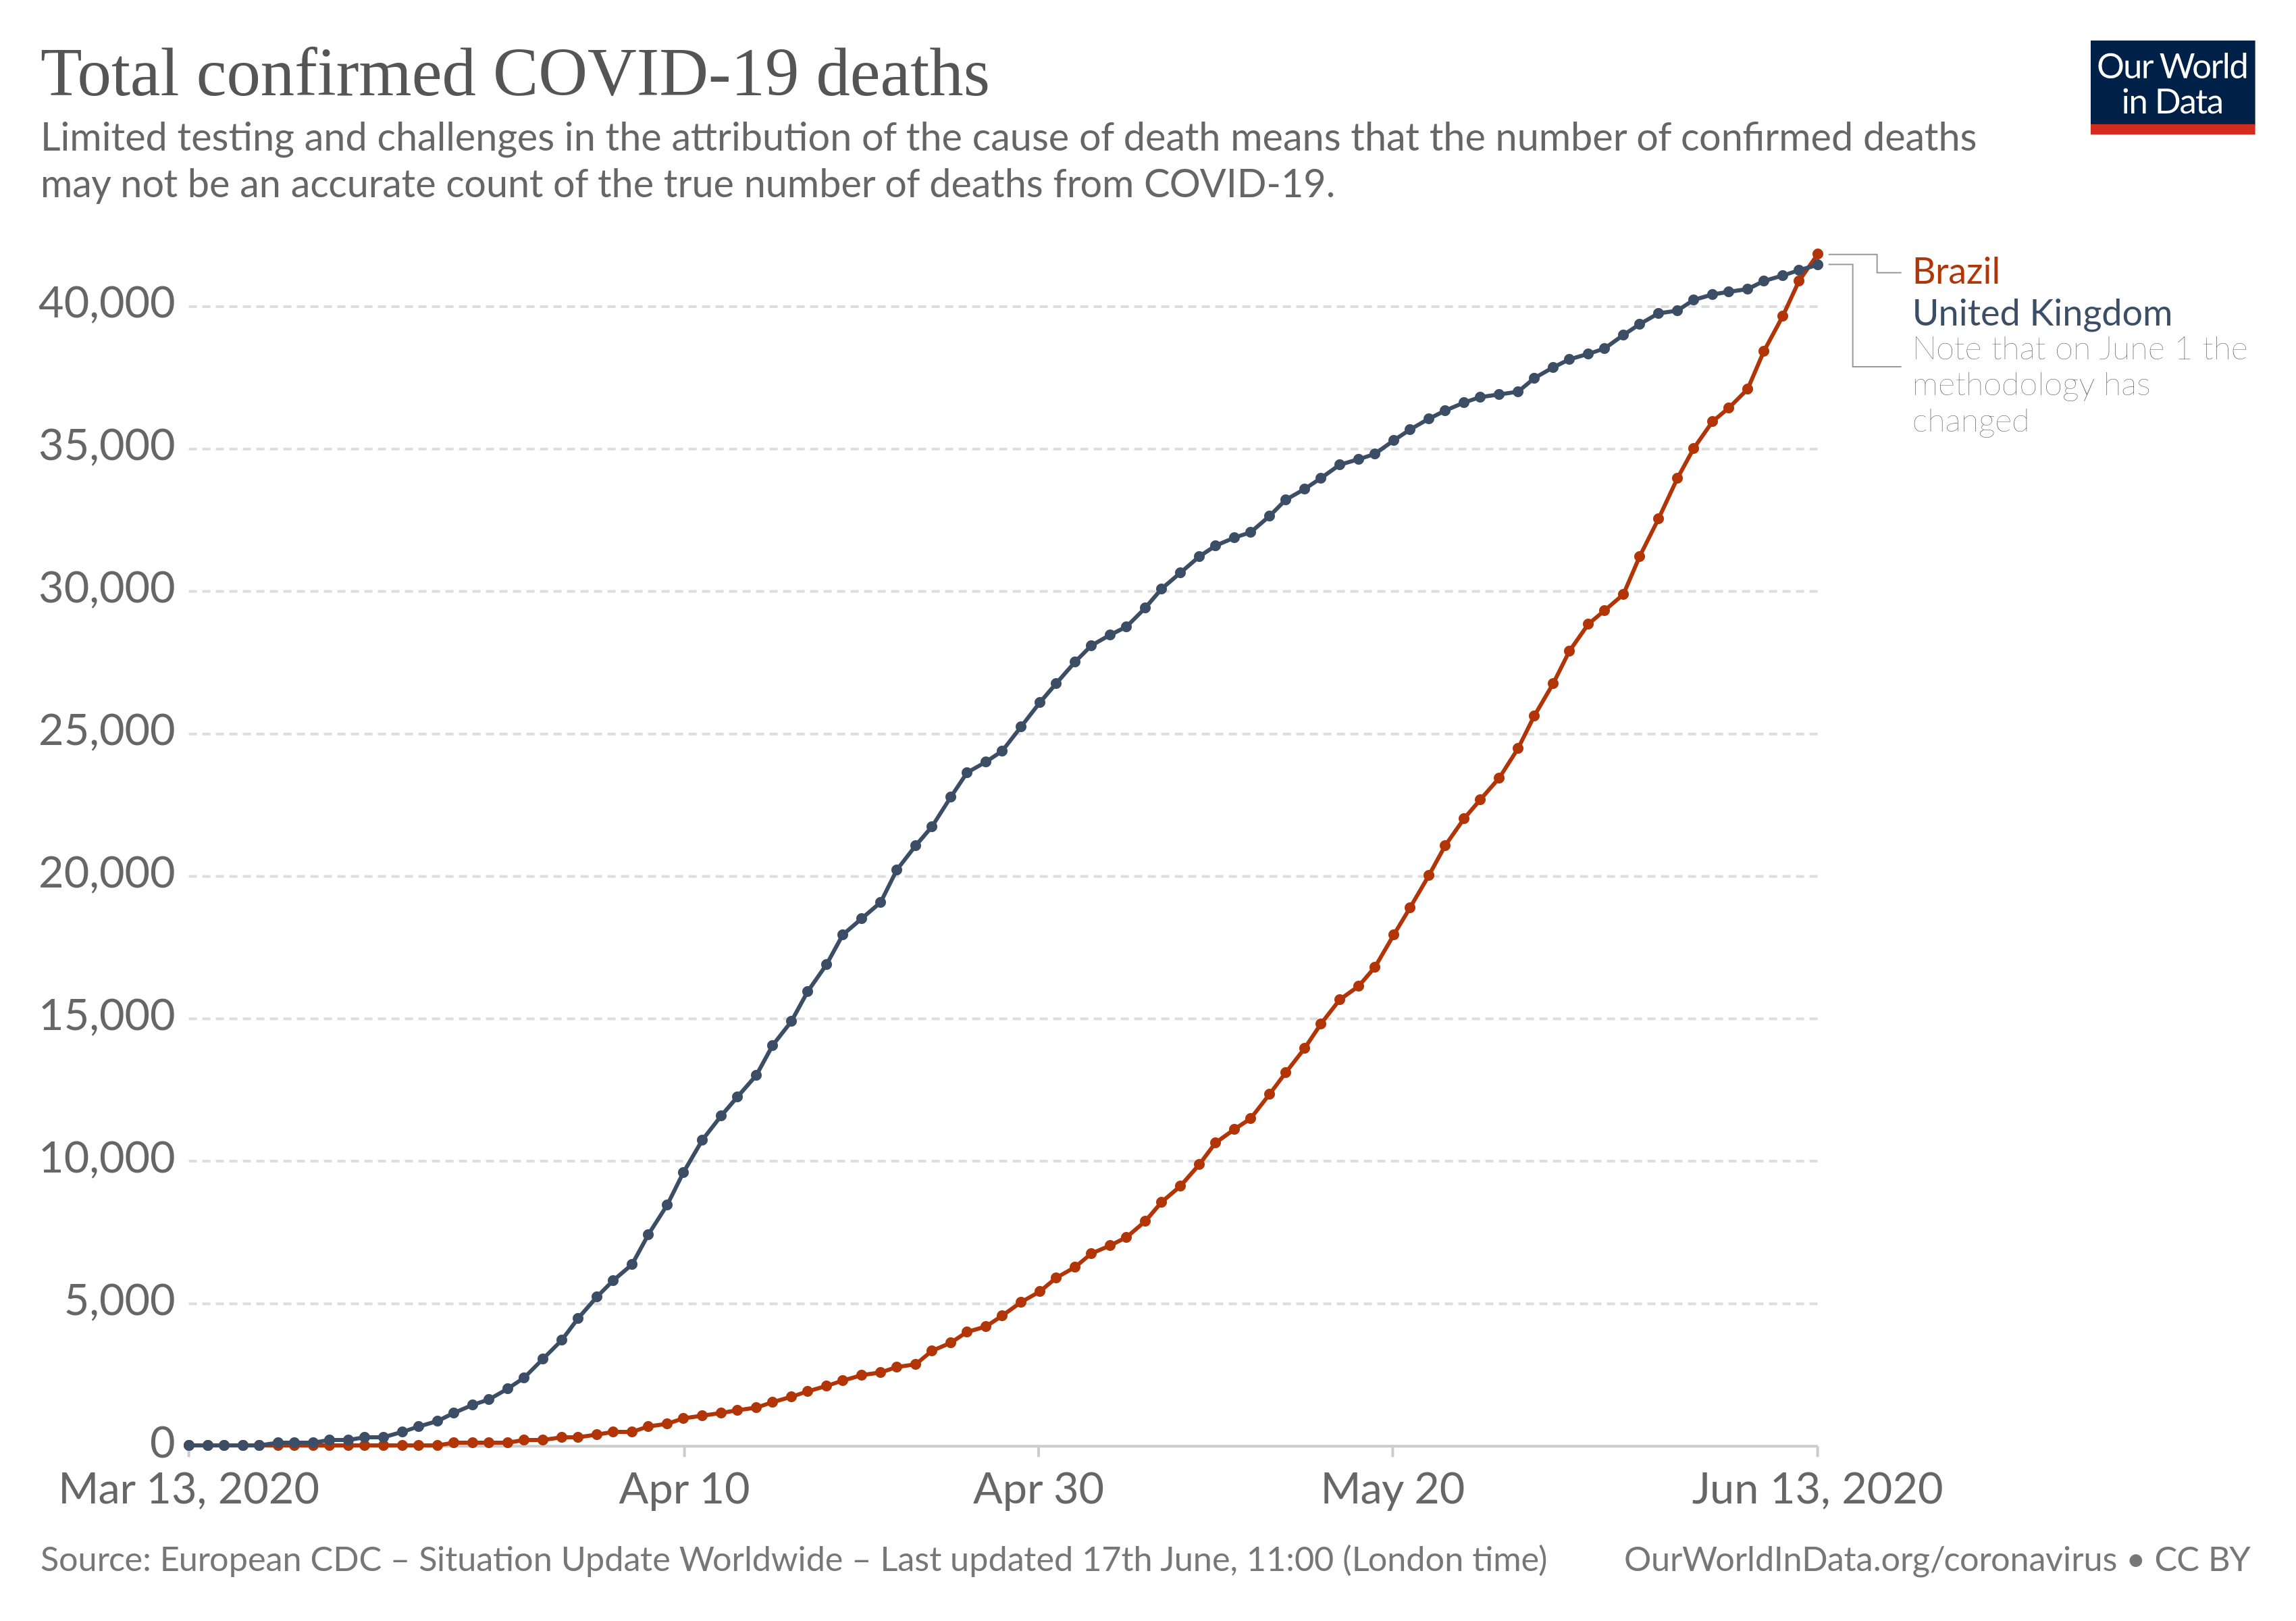
\includegraphics[width=0.8\linewidth]{Figuras/Brasil_Inglaterra_mortes.png}

\textbf{Fonte:} \textit{Our World in Data} (ourworldindata.org).
\end{center}
\end{task}



\explore{Funções logarítmicas e exponenciais}

\begin{ObjetivoEsp}
{Logarítmicas e exponenciais}
{Analisar e estabelecer relações entre as representações de funções exponencial e logarítmica (EM13MAT403).}
{1}
\end{ObjetivoEsp}

\begin{Recomenda}
{Logarítmicas e exponenciais}
{A exploração propõem a utilização do \textit{applet} do GeoGebra no celular ou no computador, o que recomenda-se fortemente. Não sendo possível a utilização do \textit{applet}, pode-se falar do gráfico mostrado e explicar que a mesma simetria vale para outras bases.

Espera-se que os alunos estejam intrigados com a simetria nos gráficos das funções exponenciais e logarítmicas. Recomenda-se, então, que se recorde que um ponto $(x,y)$ pertence ao gráfico da função $a^x$, se $y=a^x$. Então o logaritmo desse $y$ em base $a$ só pode ser $x$, que é o expoente ao qual $a$ foi elevado para obter-se $y$, o que garante que o ponto $(y,x)$ está no gráfico de $\log_a y$. De modo semelhante, se um ponto $(y,x)$ está no gráfico de $\log_a y$, então $x$ é o expoente ao qual devemos elevar $a$ para obter $y$ e $a^x=y$, de modo que $(x,y)$ está no gráfico de $a^x$.}
{1}
\end{Recomenda}

O gráfico abaixo ilustra as funções $f(x)=2^x$ (verde), $g(x)=\log_2 x$ (azul) e a função $h(x)=x$
\begin{center}
\centering
\captionof{figure}{Funções exponencial e logarítmica de mesma base.}
\includegraphics[width=0.8\linewidth]{Figuras/Fun_Exp_Log.png}
\end{center}

Para qualquer base $a>0$, $a \neq 1$, temos que $f(x)=a^x$ e $g(x)=\log_a x$ são simétricas em relação à função $h(x)=x$. Podemos utilizar um computador ou celular para acessar a atividade do GeoGebra abaixo e verificar, utilizando o controle deslizante, que essa simetria verifica-se para as mais diversas bases.

https://www.geogebra.org/calculator/wx7fkdk7 \begin{minipage}{0.3\linewidth}
\includegraphics[width=\linewidth]{Figuras/QRcode_exp_log.png}\end{minipage}

\begin{ObjetivoEsp}{Para pesquisar}
{Perceber que a função logarítmica não está definida quando o valor da base é igual a 1.}
{1}
\end{ObjetivoEsp}

\begin{resposta}{Para pesquisar}
{O gráfico de $a^x$ torna-se constante igual a 1 e o gráfico do $\log_a x$ desaparece. Isso ocorre pois, para $a=1$, temos $f(x)=1^x =1$ para todo $x \in \mathbb{R}$, de modo que $\log_1 x$ não existe para $x \neq 1$.}
{1}
\end{resposta}

\begin{research}
Utilize o applet do geogebra para investigar o que ocorre com os gráficos de $f(x)=a^x$ e $g(x)=\log_a x$ quando $a=1$. Por que você acha que isso ocorre?
\end{research}



\begin{observation}{O logaritmo e a exponencial são inversas}
Se um ponto $(x,y)$ está no gráfico da função exponencial de base $a$, então $y= a^x$. Agora, se calcularmos $\log_a y$ obtemos $x$ (pois $x$ é o expoente ao qual devemos elevar $a$ para obter $y$), de modo que o ponto $(y,x)$ está no gráfico da função logarítmica de base $a$. Essa simetria traduz, então, o fato das funções logarítmicas e exponenciais serem inversas: dada uma base real $a>0$, $a \neq 1$, e números reais $x>0$ e $y$ qualquer, temos
\begin{align*}
& a^{\log_a x}=x,\\
& \log_a (a^y) = y.
\end{align*}
\end{observation}

\begin{Recomenda}{Funções inversas na prática}
{A troca nos papeis de $x$ e $y$ como argumentos das funções pode causar dificuldade e pode ser necessário relembrar que uma função age sobre seu argumento, independente das variáveis que sejam utilizadas.

A atividade propõem colocar a "mão na massa" na exponencial e no logaritmo, observando a ação da inversão explicitada na observação anterior.}
{1}
\end{Recomenda}

\begin{resposta}{Inversas na prática}
{\begin{center}
\begin{tabular}{|c|c|c||c|c|c|}
\hline
$x$ & \cellcolor[HTML]{00A59D} $y=2^x$ & \cellcolor[HTML]{00A59D}  $\log_2 y$ & $y$ & \cellcolor[HTML]{00A59D} $x=3^y$ & \cellcolor[HTML]{00A59D}  $\log_3 x$ \\
\hline \hline 1 & 2 & 1 &-1 & 1/3 & -1 \\
\hline 2 & 4 & 2 & 1 & 3 & 1 \\
\hline 3 & 8 & 3 & 0 & 1 & 0 \\
\hline 4 & 16 & 4 & 2 & 9 & 2 \\
\hline
\end{tabular}
\end{center}}
{1}
\end{resposta}

\begin{task}{Funções inversas na prática}
Complete a tabela abaixo calculando a exponencial do logaritmo e o logaritmo da exponencial.
\begin{center}
\begin{tabular}{|c|c|c||c|c|c|}
\hline
$x$ & \cellcolor[HTML]{00A59D} $y=2^x$ & \cellcolor[HTML]{00A59D}  $\log_2 y$ & $y$ & \cellcolor[HTML]{00A59D} $x=3^y$ & \cellcolor[HTML]{00A59D}  $\log_3 x$ \\
\hline \hline 1 &  & &-1 & & \\
\hline 2 &  &  & 1 & & \\
\hline 3 &  &  & 0 & & \\
\hline 4 & &  & 2 & & \\
\hline
\end{tabular}
\end{center}
\end{task}

\begin{Recomenda}{Para refletir}
{A reflexão proposta busca levar o aluno a expressar o significado da inversão das funções como inversa uma da outra e pode ser usada para avaliar se houve compreensão do argumento para a simetria do gráfico.
}
{1}
\end{Recomenda}

\begin{reflection}
Você consegue explicar por que $a^{\log_a x}=x$ e $\log_a (a^y) = y$? Tente discutir com seus colegas por que essas igualdades valem.
\end{reflection}

\begin{resposta}{Para refletir}
{Espera-se respostas como "$a^{\log_a x}=x$ porque o logaritmo é o expoente ao qual devemos elevar $a$ para obter $x$" e "$\log_a (a^y)=y$ porque $y$ é o expoente ao qual devemos elevar $a$ para obter $a^y$".}
{1}
\end{resposta}

Uma consequência do fato de que as funções logarítmicas e exponenciais são inversas, é que funções logarítmicas de bases distintas são muito parecidas. É possível multiplicar uma delas por uma constante para obter a outra.

\begin{Recomenda}{Funções logarítmicas distintas}
{Por fim é proposta outra atividade no GeoGebra, que pretende mostrar que trocar de base é o mesmo que multiplicar a função logarítmica por uma constante, que é ressaltada na observação seguinte. Não havendo a possibilidade de usar o \textit{applet}, essa atividade poderia ser deixada de lado e a conclusão poderia ser reforçada como interpretação da equação $\log_a x = \log_a b \log_b x$.}
{1}
\end{Recomenda}

\begin{task}{Funções logarítmicas distintas}
No \textit{applet} do GeoGebra, disponível através do atalho abaixo, podemos mover a barra com o valor $a$, alterando o gráfico da função $h(x) = a \log_2 x$. Qual o valor de $a$ para que o gráfico de $h(x)$ coincida com o gráfico de $f(x) = \log_{1{,}2} x$?

https://www.geogebra.org/calculator/qyuzhbmp \begin{minipage}{0.3\linewidth}
\includegraphics[width=\linewidth]{Figuras/QRcode_mult_constante.png}\end{minipage}

\textbf{Desafio:} aplique o Teorema da mudança de base em $g(x)= \log_2 x$, utilizando a base $1{,}2$ para encontrar algebricamente o valor de $a$.
\end{task}

\begin{resposta}{Funções logarítmicas distintas}
{$a = 3{,}8$, que é uma aproximação muito boa para $\log_{1{,}2}2 \approx 3{,}8017840169239$, que é a resposta do desafio.}
{1}
\end{resposta}


\begin{ObjetivoEsp}{Funções de bases distintas}
{Reconhecer o perfil de funções logarítmicas de bases distintas.
}
{1}
\end{ObjetivoEsp}

\begin{Recomenda}{Funções de bases distintas}
{O gráfico ilustra diversas funções logarítmicas simultaneamente e recomenda-se que destaque-se duas características:
\begin{itemize}
\item As linhas laranjas representam os gráficos das funções logarítmicas de base maior do que 1, sendo que quanto maior a base, menores são os valores dos logaritmos. Assim o gráfico a função de maior base é a linha laranja mais próxima do eixo $x$ e a de menor base (mas ainda maior do que 1) é aquela que cresce mais rapidamente, ultrapassando os valores do gráfico logo após o número 1.
\item As linhas verdes representam os gráficos das funções logarítmicas de base menor do que 1 (mas ainda maior do que 0), sendo que quanto mais próxima de 1 a base for, maiores em módulo são os valores dos logaritmos. Assim o gráfico da função de menor base (no intervalo $(0,1)$) é a mais próxima do eixo $x$ e a função de maior base (mas ainda menor do que 1) é a linha verde que diminui mais rapidamente, ficando menor do que os valores do gráfico logo após o número 1.
\end{itemize}
Recomenda-se que se aponte o fato que as funções logarítmicas de base maior do que 1 são crescentes e que funções logarítmicas de base menor do que 1 são decrescentes. O fato em si é importante, inclusive para as aplicações, mas a demonstração só é recomendada se a turma dominar o conceito de função crescente. Pode-se ressaltar que esse fato já estava aparente nas tabelas de logaritmos anteriores.}
{0}
\end{Recomenda}

\begin{observation}{Funções logarítmicas de bases distintas}
Podemos utilizar o fato das funções exponenciais e logarítmicas serem inversas para trocar as bases de funções logarítmicas:
\begin{align*}
&\log_a x = \log_a b^{\log_b x} =\log_a b\log_b x.
\end{align*}
Ou seja a função $\log_a x$ é igual à função $\log_b x$ multiplicada pela constante $\log_a b$. Essa constante pode ser negativa se $a<b$.
\end{observation}

A figura abaixo ilustra os gráficos de funções logarítmicas de bases distintas (base maior do que 1 na cor laranja e menor do que 1 na cor verde).

\begin{figure}[!htb]
\centering
\caption{Funções logarítmicas de bases distintas.}
\includegraphics[width=0.8\linewidth]{Figuras/Graficos_logs.png}
\end{figure}


\begin{ObjetivoEsp}{Crescentes e decrescentes}
{Comprovar que funções logarítmicas de base maior do que 1 são crescentes e que funções logarítmicas de base menor do que 1 são decrescentes.}
{1}
\end{ObjetivoEsp}

\begin{observation}{Funções logarítmicas crescentes e decrescentes}
Observamos na figura, imediatamente, que as funções logarítmicas de base maior do que 1 são crescentes. Isso ocorre porque as exponenciais de base $a>1$ são funções estritamente crescentes:
$$
x > y \Longleftrightarrow a^x > a^y,
$$
ou seja, para $x=\log_a c$ e $y=\log_a d$, temos
$$
\log_a c > \log_a d \Longleftrightarrow c > d.
$$
Também observamos que as funções logarítmicas de base menor do que 1 são decrescentes. Isso ocorre porque as exponenciais de base $b<1$ são funções estritamente decrescentes:
$$
x > y \Longleftrightarrow b^x < b^y,
$$
ou seja, para $x=\log_b c$ e $y=\log_b d$, temos
$$
\log_b c > \log_b d \Longleftrightarrow c < d.
$$


\end{observation}


\exercise

\begin{ObjetivoEsp}{Exercícios}
{Resolver exercícios contextualizados.}
{1}
\end{ObjetivoEsp}

\begin{resposta}{\ref{EstimaGraf} - Estimando com o gráfico}
{Comparando os valores da função para $m$ igual a 200, 300 e 400 com as linhas da grade, observamos:
\begin{enumerate}[label=\alph*)]
\item $80>f(200)>60$, de modo que 70 é uma estimativa adequada;
\item $120>f(300)>100$, de modo que 110 é uma estimativa adequada;
\item $140>f(400)>120$, de modo que 130 é uma estimativa adequada.
\end{enumerate}}
{1}
\end{resposta}

\begin{resposta}{\ref{poluicaoSonora} - Poluição Sonora}
{\begin{align*}
& 35 = 10 \log(I \times 10^{12}) \Rightarrow   3{,}5 = \log I + 12\\
\Rightarrow & -8{,}5 = \log I \Rightarrow I = 10^{-8{,}5}
\end{align*}}
{1}
\end{resposta}

\begin{resposta}{\ref{UFC2001} - (UFC-2001)}
{\begin{align*}
& 80 = 120+10 \log I_1 \Rightarrow  -40 = 10\log I_1\\
\Rightarrow & I_1 = 10^{-4},
\end{align*}
\begin{align*}
& 60 = 120+10 \log I_2 \Rightarrow -60 = 10\log I_2\\
\Rightarrow & I_2 = 10^{-6},
\end{align*}
Assim
$$
\frac{I_1}{I_2}=\frac{10^{-4}}{10^{-6}}= 100.
$$}
{1}
\end{resposta}

\begin{resposta}{\ref{Unesp2006} - (Unesp-2006)}
{\begin{align*}
 20 =& N_1-N_2 = 120 +10\log I_1- (120 +10\log I_1) \\
 =& 10\log I_1 - \log I_2 = 10\log (I_1/I_2)\\
\Rightarrow I_1/I_2  =& 10^{2}
\end{align*}}
{1}
\end{resposta}

\begin{resposta}{\ref{Unicamp2008} - (Unicamp-2008)}
{\begin{itemize}
\item[(1)] Verdadeira pois
$$
0 = 10(12+\log I) \Rightarrow I = 10^{-12}
$$
\item[(2)] Falsa pois a intensidade do ruído do avião a jato é
$$
160 = 10(12+\log I) \Rightarrow I = 10^{4},
$$
enquanto a intensidade do ruído do tráfego é
$$
80 = 10(12+\log I) \Rightarrow I = 10^{-4}.
$$
Assim a intensidade do ruído do avião é 100 milhões ($10^8$) de vezes maior do que a intensidade do ruído da esquina movimentada.
\item[(3)] Verdadeira, de acordo com o enunciado da questão, pois essa é a intensidade sonora da esquina movimentada.
Assim a intensidade do ruído do avião é 100 milhões ($10^8$) de vezes maior do que a intensidade do ruído da esquina movimentada.
\end{itemize}}
{1}
\end{resposta}


\begin{resposta}{\ref{UCSSRS} - (UCS-RS)}
{$\beta$ aumenta em 20 decibéis pois
\begin{align*}
\beta =& 10\log(100 I/I_0) = 10(\log 100 + \log(I/I_0))\\
=& 20 + 10\log(I/I_0).
\end{align*}}
{1}
\end{resposta}


\begin{enumerate}
\item {} \label{EstimaGraf}

É possível verificar rapidamente, utilizando gráficos, o tempo que uma aplicação demora para dobrar, triplicar, quadruplicar, ... o valor aplicado. O gráfico abaixo, da função $f(m)=\log_{1{,}01}(m/100)$, representa o tempo, em meses, para que determinado montante seja atingido a partir de um capital de $R\$ 100{,}00$, aplicado a uma taxa mensal de $1\%$.  Observando o gráfico, estime com erro menor do que $10$ o número de meses necessário para o capital inicial:
\begin{enumerate}
\item dobrar;
\item triplicar;
\item quadruplicar.
\end{enumerate}
\begin{center}
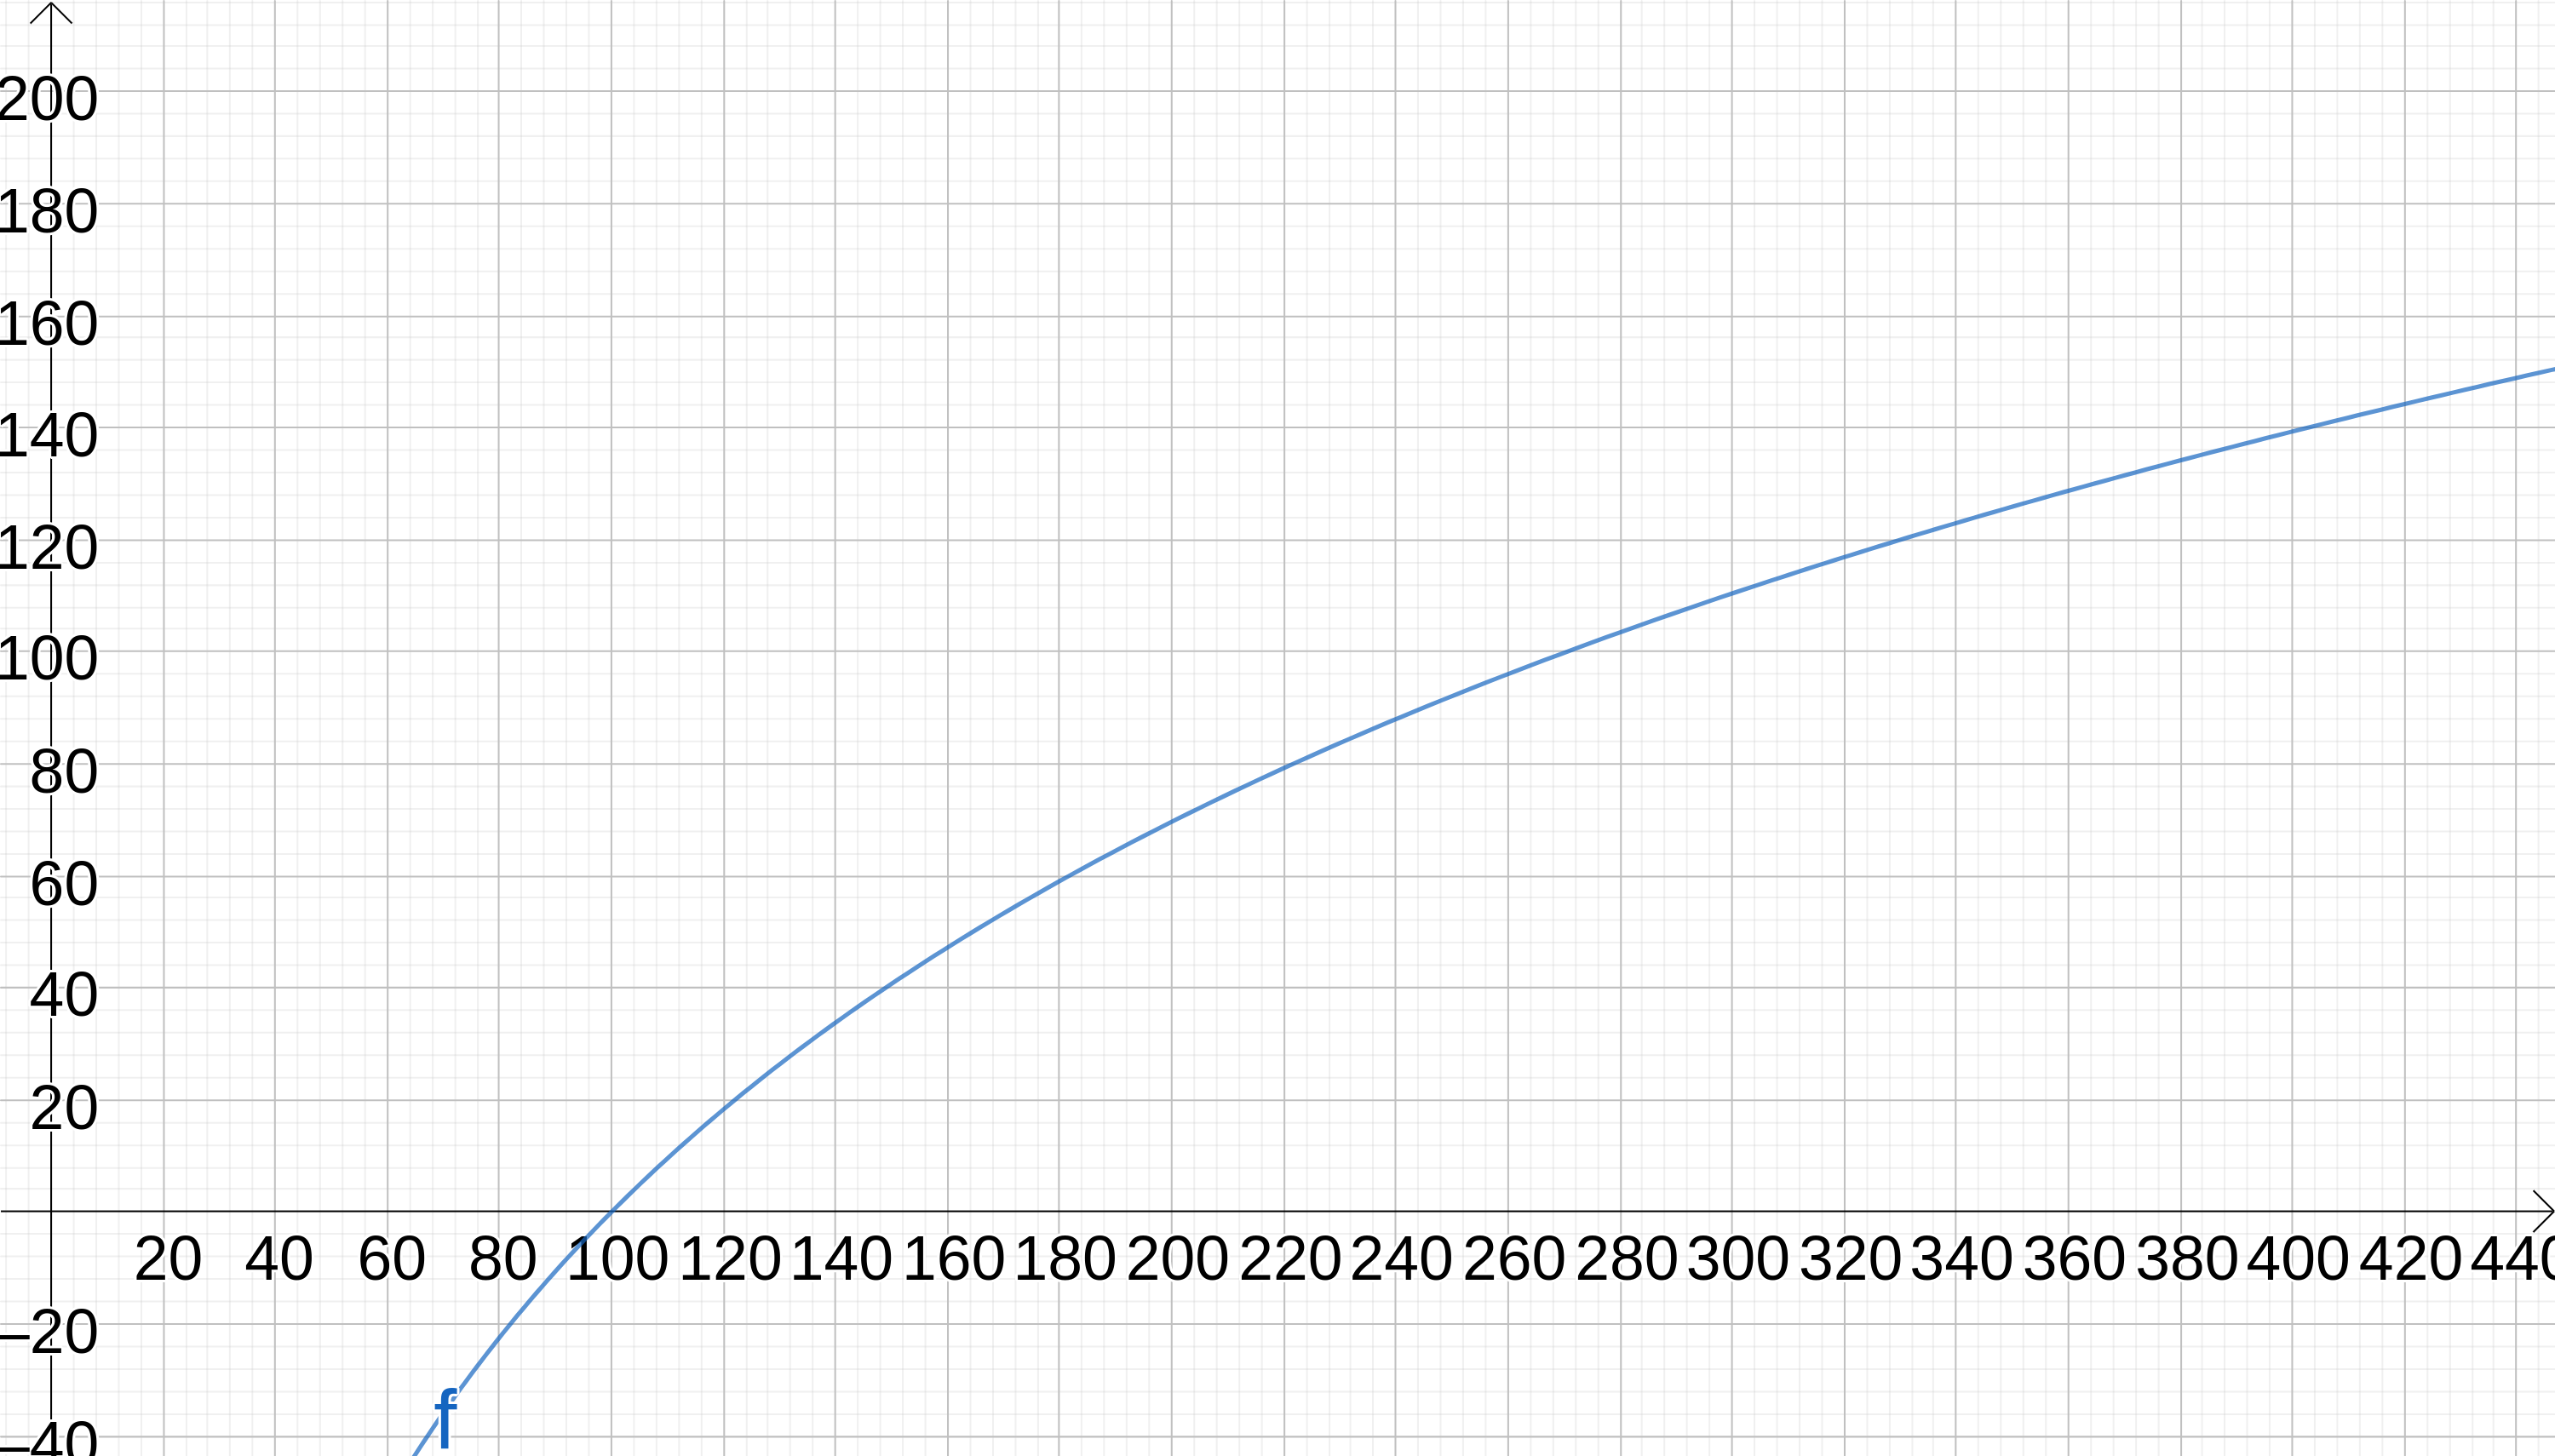
\includegraphics[width=0.8\linewidth]{Figuras/Tempo_montante.png}
\captionof{figure}{Gráfico da função $f(m)=\log_{1{,}01} (m/100)$.}
\end{center}


\item {}\label{poluicaoSonora}

\textbf{(Poluição sonora em sala de aula)} Um teste feito com um decibelímetro em uma escola, em São Carlos (SP), 
constatou que o nível de ruído emitido pelas crianças dentro de sala de aula está acima do recomendado pela Organização 
Mundial de Saúde  (OMS) e a Associação Brasileira de Normas Técnicas. A exposição a esses ruídos podem prejudicar o 
aprendizado e causar danos ao aparelho auditivo, de acordo com especialistas.
Segundo a OMS, o nível seguro de ruído em uma sala de aula não pode ultrapassar os 35 decibéis. Já para a Associação Brasileira de Normas Técnicas, o limite é de 50 decibéis.

A reportagem do Jornal da EPTV utilizou um decibelímetro para fazer a medição e o resultado em uma sala de aula chegou a 74 decibéis. O sinal da escola também ficou acima do recomendado, registrando o mesmo número. Em ambientes abertos, como o pátio, os especialistas afirmam que a tolerância é um pouco maior e os sons de até 85 decibéis não trazem riscos. “Acima de 85 decibéis e oito horas de exposição já causa lesão ao aparelho auditivo”, alerta 
o médico da Universidade de São Carlos (UFSCar), Bernardino Alves Souto.

Ainda de acordo com Souto, nível acima de 75 decibéis já se pode causar alguns sintomas. "Irritabilidade, 
insônia, 
ansiedade e dificuldade de concentração, dependendo do tempo de exposição ao barulho. Em uma sala de aula com 
aproximadamente 80 decibéis de intensidade de som, a capacidade de aprendizado e concentração da criança pode reduzir de 
20{\%} a 80{\%}”, explicou 
Souto.\footnote{Fonte:\url{
http://g1.globo.com/sp/sao-carlos-regiao/noticia/2014/01/nivel-de-ruido-em-escola-esta-acima-do-recomendado-em-sao-carlo
s-sp.html}. Acesso em: 25 set. 2017.}

 O nível sonoro (NS), medido em decibel (dB), pode ser calculado usando a fórmula $NS=10\cdot log(\frac{I}{I_0})$ onde I 
é a intensidade do som considerado e $I_0$ é a menor intensidade sonara audível, sendo  $I_0=10^{-12}$ $W/m^2$. 
Considerando 35 decibéis o nível sonoro ideal em uma sala de aula, determine a intensidade do som nesse ambiente.




\item {}\label{UFC2001}

(UFC-2001) Suponha que o nível sonoro $\beta$ e a intensidade I de um som estejam relacionados pela equação logarítmica 
$\beta = 120 + 10\cdot log_{10} I$, em que b é medido em decibéis e I, em watts por metro quadrado. Sejam $I_1$ a 
intensidade correspondente ao nível sonoro de 80 decibéis de um cruzamento de duas avenidas movimentadas e $I_2$ a 
intensidade correspondente ao nível sonoro de 60 decibéis do interior de um automóvel com ar-condicionado. A razão 
$I_1/I_2$ é igual a:
 \begin{enumerate}
     \item 1/10
     \item 1
     \item 10 
     \item 100
     \item 1 000
 \end{enumerate}


\item {}\label{Unesp2006}

(Unesp-2006) O nível sonoro N, medido em decibéis (dB) e a intensidade I de um som, medida em watt por metro quadrado 
($W/m_2$), estão relacionados pela equação $N=120+10\cdot \log_{10} (I)$. Suponha que foram medidos, em certo local, os 
níveis sonoros, $N_1$ e $N_2$, de dois ruídos com Intensidades $I_1$ e $I_2$, respectivamente. Sendo $N_1 - N_2 = 20 dB$, 
a razão $I_1/I_2$ é:
\begin{enumerate}
    \item $10^{-2}$
    \item $10^{-1}$
     \item $10$
     \item $10^{2}$
     \item $10^{3}$
\end{enumerate}





\item {} \label{Unicamp2008}

(Unicamp-2008) A escala de um aparelho para medir ruídos é definida da seguinte forma: $R = 12 + log_{10}(I)$, em que R 
é a medida do ruído, em bels, e I é a intensidade sonora, em W/m2. No Brasil, a unidade utilizada é o decibel (1/10 do 
bel). Por exemplo, o ruído dos motores de um avião a jato é de 160 decibéis, enquanto o ruído do tráfego em uma esquina 
movimentada de uma grande cidade é de 80 decibéis, sendo este o limite a partir do qual o ruído passa a ser nocivo ao 
ouvido humano. Com base nessas informações, julgue os itens que se seguem.

(1) A intensidade sonora de um ruído de zero decibel é de $10^{-12} w/m^2$. 

(2) A intensidade sonora dos motores de um avião a jato é o dobro da intensidade sonora do tráfego em uma esquina movimentada de uma grande cidade.

(3) Uma intensidade sonora maior que $10^{-4} w/m^2$ produz um ruído que é nocivo ao ouvido humano. 




\item {}\label{UCSSRS}

(UCS-RS) O nível $\beta$, em decibel, de um som que tem intensidade I é dado pela fórmula $\beta = 10 \cdot log 
(I/I_0)$, em que $I_0 = 10^{-12}$. Se a intensidade I for multiplicada por 100, em quantos decibel aumenta $\beta$?

\begin{enumerate}
    \item 2
    \item 20
    \item 100
    \item 120
    \item 140
\end{enumerate}
\end{enumerate}


\explore{Escala logarítmica}

\begin{ObjetivoEsp}{Escala logarítmica}
{\begin{itemize}
\item Reconhecer a inadequação de gráficos em escala linear para dados de magnitudes muito distintas.
\item Representar dados em escala logarítmica.
\end{itemize}}
{1}
\end{ObjetivoEsp}

\begin{Recomenda}{Escala logarítmica}
{Gráficos em escala logarítmica estão presentes em muitas áreas da ciência. Esses gráficos são utilizados, por exemplo, quando temos dados de magnitude muito distinta em uma mesma análise ou quando crescimentos relativos (ou percentuais) são mais importantes do que os valores absolutos do crescimento, como no caso de ações da bolsa. 

Essa exploração propõem comparar a apresentação dos planetas do sistema solar e do sol na escala linear e na escala logarítmica. Pode ser interessante explicar aos estudantes que muitas imagens na astronomia utilizam escalas logarítmicas. Em representações do sistema solar, frequentemente utiliza-se uma escala logarítmica para as distâncias dos planetas, o que não foi feito nas figuras ao lado, e outra escala logarítmica para os tamanhos dos planetas. Isso ocorre pois as distâncias no sistema solar são muito maiores do que os tamanhos dos planetas e do sol. Seria possível aproveitar o assunto para uma exploração interdisciplinar, junto com a/o docente de física, sobre o sistema solar (incluindo as distâncias entre os objetos e suas magnitudes).
}
{1}
\end{Recomenda}

Às vezes, em situações concretas, podemos ter magnitudes muito diferentes dentro de um conjunto de valores. Na figura abaixo, por exemplo, as circunferências têm raios proporcionais aos raios do Sol (amarelo) e dos 8 planetas do sistema solar: Mercúrio (cinza, muito pequeno para ver), Vênus (rosa), Terra (azul pálido), Marte (vermelho), Júpiter (amarelo queimado), Saturno (laranja), Urano (azul claro) e Netuno (azul).

\captionof{figure}{O sol e os planetas em escala linear (em milhares de quilômetros).}
\resizebox{\textwidth}{!}{
\begin{tikzpicture}[background rectangle/.style={fill=black}, show background rectangle]
\draw[fill=yellow] (0,0) circle [radius=6.963];
\draw[fill=gray] (7.2,0) circle [radius=0.024];
\draw[fill=pink] (7.5,0) circle [radius=0.0605];
\draw[fill=blue!60!white] (7.8,0) circle [radius=0.0637];
\draw[fill=red] (8.1,0) circle [radius=0.034];
\draw[fill=olive!40!orange] (9,0) circle [radius=0.69911];
\draw[fill=olive!20!orange] (10.4,0) circle [radius=0.58232];
\draw[fill=blue!30!white] (11.4,0) circle [radius=0.253];
\draw[fill=blue] (12,0) circle [radius=0.246];
\draw[color=white](-7.2,1)--(-7.5,1)node[color=white,left,font=\large]{100};  
\draw[color=white](-7.2,5)--(-7.5,5)node[color=white,left,font=\large]{500};     
\draw[color=white](-7.2,0)--(-7.5,0)node[color=white,left,font=\large]{0};
\draw[color=white](-7.2,0)--(-7.2,7);
\end{tikzpicture}}

É muito difícil ver os planetas menores na figura. Para lidar com dados de magnitudes muito distintas, com frequência, utiliza-se uma escala logarítmica (a mesma da régua de cálculo). Na figura abaixo observamos os mesmos objetos em uma escala logarítmica (branca).

\captionof{figure}{O sol e os planetas em escala logarítmica (em milhares de quilômetros).}\label{log_planetas}
\resizebox{\textwidth}{!}{
\begin{tikzpicture}[background rectangle/.style={fill=black}, show background rectangle]
\draw[fill=yellow] (0,0) circle [radius=(ln(696.3)/ln(10))];
\draw[fill=gray] (3.4,0) circle [radius=(ln(2.4)/ln(10))];
\draw[fill=pink] (4.8,0) circle [radius=(ln(6.05)/ln(10))];
\draw[fill=blue!60!white] (6.6,0) circle [radius=(ln(6.38)/ln(10))];
\draw[fill=red] (8.1,0) circle [radius=(ln(3.4)/ln(10))];
\draw[fill=olive!40!orange] (10.7,0) circle [radius=(ln(69.911)/ln(10))];
\draw[fill=olive!20!orange] (14.7,0) circle [radius=(ln(58.232)/ln(10))];
\draw[fill=blue!30!white] (18,0) circle [radius=(ln(25.3)/ln(10))];
\draw[fill=blue] (21,0) circle [radius=(ln(24.6)/ln(10))];
\draw[color=white](-3,2)--(-3.2,2)node[color=white,left,font=\large]{100};  
\draw[color=white](-3,3)--(-3.2,3)node[color=white,left,font=\large]{1000};  
\draw[color=white](-3,1)--(-3.2,1)node[color=white,left,font=\large]{10};     
\draw[color=white](-3,0)--(-3.2,0)node[color=white,left,font=\large]{0};
\draw[color=white](-3,0)--(-3,3);
\draw[color=gray](-4.5,2)--(-4.7,2)node[color=gray,left,font=\large]{2};  
\draw[color=gray](-4.5,3)--(-4.7,3)node[color=gray,left,font=\large]{3};  
\draw[color=gray](-4.5,1)--(-4.7,1)node[color=gray,left,font=\large]{1};     
%\draw[color=gray](-10.2,0)--(-10.7,0)node[color=gray,left,font=\Huge]{0};
\draw[color=gray](-4.5,0)--(-4.5,3);
\end{tikzpicture}}

Na escala logarítmica da figura, a cada unidade linear (cinza) os valores são \textit{multiplicados} por 10, de modo que os raios dos planetas têm valores correspondentes à escala logarítmica (branca).


\begin{observation}{Colocar um gráfico em escala logarítmica.}
A escala cinza na Figura \ref{log_planetas} explica o que fizemos para colocar o gráfico em escala logarítmica: calculamos os logaritmos dos raios dos planetas e fizemos novas circunferências com raios iguais a esses logaritmos. Como os valores da escala são as potências de 10 dos valores da escada linear, os logaritmos são exatamente os valores necessários para obter-se os respectivos valores originais nessa nova escala.
\end{observation}

\begin{ObjetivoEsp}{Ordens de magnitude.}
{Compreender corretamente a magnitude de dados em um gráfico em escala logarítmica.}
{1}
\end{ObjetivoEsp}


\begin{Recomenda}{Ordens de magnitude.}
{A atividade "Ordens de magnitude dos planetas" pode ser realizada como uma discussão em grupo e pretende que seja discutida a interpretação correta dos dados nessa escala.}
{1}
\end{Recomenda}


\begin{task}{Ordens de magnitude dos planetas.}
Observado as circunferências e a escala logarítmica da Figura \ref{log_planetas}, qual é a melhor aproximação na comparação dos tamanhos de Vênus (rosa) e de Saturno (laranja).
\begin{enumerate}
\item O diâmetro de Saturno é o dobro do diâmetro de Vênus.
\item O diâmetro de Saturno é dez vezes o diâmetro de Vênus.
\item O diâmetro de Saturno é três vezes o diâmetro de Vênus.
\item O diâmetro de Saturno é cem vezes o diâmetro de Vênus.
\end{enumerate}
\end{task}

\begin{resposta}{Ordens de magnitude dos planetas.}
{A observação do gráfico pode ser difícil de traduzir em termos numéricos diretamente e é possível tentar responder a questão de duas maneiras:
\begin{itemize}
\item O raio de Vênus está na parte superior ($\log 5 \approx 0{,}7$) do intervalo [0, 10], o que indica que o raio está no intervalo [5, 10], e o raio de Saturno está na parte superior do intervalo [10, 100], o que indica que o raio está no intervalo [50, 100]. Desse modo a razão $r$ entre os raios de Saturno e Vênus estaria entre $50/10=5$ e $100/5=20$. Tomando o valor médio do intervalo [5, 20] como aproximação, que é 12.5, a resposta 10 seria a melhor das opções.
\item A distância linear (na escala logarítmica) entre os raios de Vênus e Saturno é de aproximadamente 1, o que se traduz em um aumento de 10 vezes na escala logarítmica.
\end{itemize}
O raio Saturno é de 58.232 Km e o de Vênus é de 6.051,8 Km e 10 vezes é, de fato, a melhor aproximação.}
{1}
\end{resposta}

\ifnum \aluno=1
\vspace{0mm}
\else
\vspace{-2mm}
\fi

\begin{Recomenda}{Distâncias entre os planetas.}
{A observação "Distâncias entre os planetas" objetiva evitar que os estudantes sejam induzidos ao erro, imaginando que as distâncias entre os planetas estavam em escala nas atividades anteriores.}
{1}
\end{Recomenda}

\begin{knowledge}
\textbf{Distâncias entre os planetas.}
Nas figuras acima apenas colocamos os "planetas"\, lado a lado. Não levamos em conta as distâncias entre eles. O sistema solar é muito maior do os raios  dos planetas e do próprio Sol. Para se ter uma ideia, a distância de Netuno ao Sol é de cerca de $4{,}5 \times 10^{9}Km$, enquanto o diâmetro do Sol é de $1{,}4 \times 10^6$. Ou seja, a distância de Netuno até o Sol é mais de 3000 vezes maior do que o diâmetro do Sol.
\end{knowledge}

\ifnum \aluno=1
\vspace{0mm}
\else
\vspace{-2mm}
\fi

\begin{Recomenda}{Comprimentos e massas.}
{O exemplo visa mostrar que dados concretos com grande variação podem ser difíceis de analisar em escala linear. O/A professor/a poderia ilustrar a situação com um exemplo como: na escala linear um társio (200g e 8cm) e um mico-leão-dourado (800g e 26cm) estariam muito próximos (no canto inferior esquerdo), apesar de um ser muito maior do que o outro.}
{1}
\end{Recomenda}

\ifnum \aluno=1
\vspace{0mm}
\else
\vspace{-2mm}
\fi

\begin{example}{Comprimentos e massas de primatas.}
Às vezes estudamos dados que ocorrem em uma larga escala. Isso pode fazer com que dados significativamente distintos pareçam muito próximos e, assim, dificultar a análise. Para ilustrar isso trazemos gráfico de dispersão das massas e comprimentos médios (dados de Animal Diversity Web Quaardvark (animaldiversity.ummz.umich.edu/quaardvark)) de diversas espécies de primatas em escala logarítmica e linear
\begin{center}
\captionof{figure}{Massas e comprimentos de diversos primatas}
\begin{minipage}[c]{0.49\linewidth}
\begin{center}
Em escala linear.
\end{center}
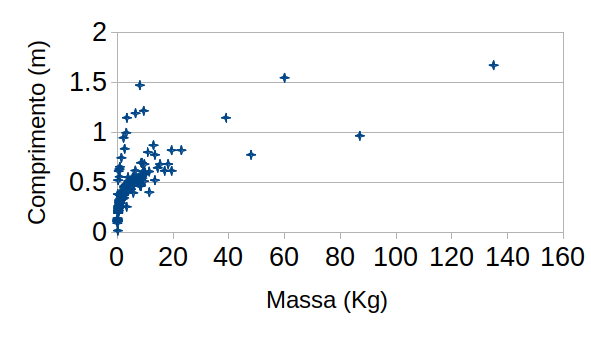
\includegraphics[width=\linewidth]{Primatas_linear.png}
\end{minipage}
\begin{minipage}[c]{0.49\linewidth}
\begin{center}
Em escala logarítmica.
\end{center}
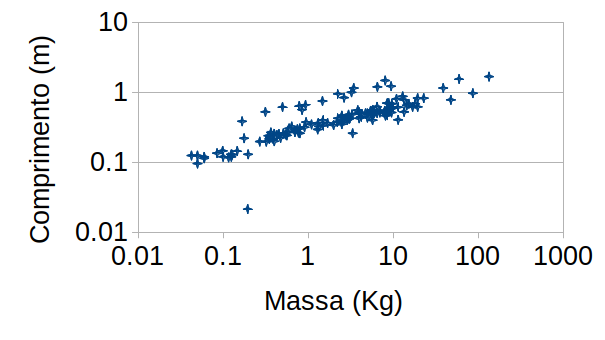
\includegraphics[width=\linewidth]{Primatas_log.png}
\end{minipage}
\end{center}
Os dados ficam, assim, mais distribuídos e melhores para análise. Muitos dos primatas têm menos de 1 Kg e menos de 50 cm, contudo um animal  100 g e 10 cm é muito menor do que um animal de 1 Kg e 50 cm.
\end{example}

\arrange{Escala logarítmica}

Ao colocarmos um gráfico em escala logarítmica parece que "espalhamos" mais os dados de menor magnitude, que estavam condensados em uma região muito pequena. Isso ocorre pois os valores nessa escala crescem mais lentamente para valores menores do que para valores maiores. %torna iguais crescimentos relativos iguais e não as magnitudes dos dados per si.

\begin{ObjetivoEsp}{Três cidades.}
{Representar dados em escala logarítmica.}
{1}
\end{ObjetivoEsp}


\begin{Recomenda}{Três cidades.}
{A atividade "Três cidades"\, propõem que os estudantes coloquem os dados em escala logarítmica e busquem algumas informações básicas. Essa atividade é uma preparação para o "Para refletir", que tem uma mensagem principal: crescimentos percentuais (ou relativos) iguais, produzem acréscimos de mesmo tamanho nos gráficos de escala logarítmica, independente da magnitude dos dados.}
{1}
\end{Recomenda}

\begin{task}{Três cidades.}
Vamos considerar as populações das cidades de Metrópolis, Smallville e Gotham City. Um censo realizado no ano 2000 verificou que elas tinham 10.000, 1.000 e 5.000 habitantes, respectivamente. Dez anos após verificou-se que elas estavam com 11.000, 2.000 e 10.000 habitantes, respectivamente. A figura da esquerda, em escala linear, apresenta as populações das cidades.
\begin{center}
\begin{minipage}[c]{0.4\linewidth}
\begin{center}
Populações em escala linear.
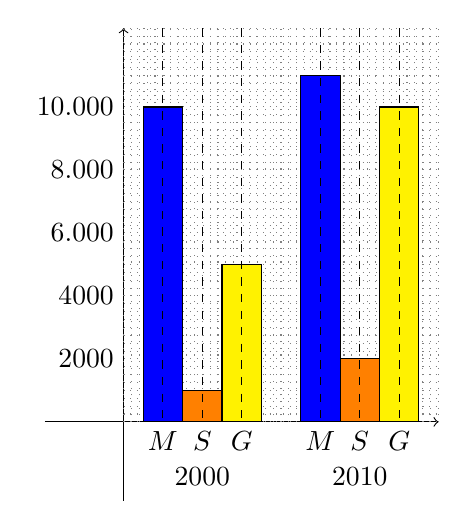
\begin{tikzpicture}[domain=0:5]
\draw[->] (-1,0) -- (4,0);
\draw[->] (0,-1) -- (0,5);
\draw[step=0.1,gray,thin, dotted] (0,0) grid (4,5);
\draw [fill=blue] (0.25,0) rectangle (0.75,4);
\draw [fill=blue] (2.25,0) rectangle (2.75,4.4);
\draw [fill=orange] (0.75,0) rectangle (1.25,0.4);
\draw [fill=orange] (2.75,0) rectangle (3.25,0.8);
\draw [fill=yellow] (1.25,0) rectangle (1.75,2);
\draw [fill=yellow] (3.25,0) rectangle (3.75,4);
\draw[dashed] (1,5) -- (1,0)node[below] {$S$};
\draw[dashed] (1.5,5) -- (1.5,0)node[below] {$G$};
\draw[dashed] (0.5,5) -- (0.5,0)node[below] {$M$};
\node at (1,-0.7) {$2000$};
\node at (3,-0.7) {$2010$};
\draw[dashed] (3,5) -- (3,0)node[below] {$S$};
\draw[dashed] (3.5,5) -- (3.5,0)node[below] {$G$};
\draw[dashed] (2.5,5) -- (2.5,0)node[below] {$M$};
\node[left] at (0,0.8) {$2000$};
\node[left] at (0,1.6) {$4000$};
\node[left] at (0,2.4) {$6.000$};
\node[left] at (0,3.2) {$8.000$};
\node[left] at (0,4) {$10.000$};
\end{tikzpicture}
\end{center}
\end{minipage}
\begin{minipage}[c]{0.4\linewidth}
\begin{center}
Populações em escala logarítmica.
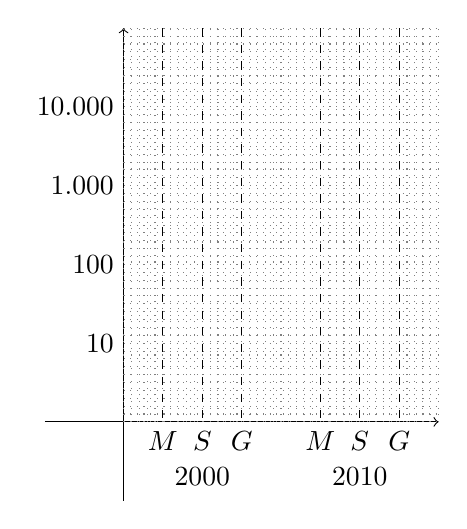
\begin{tikzpicture}[domain=0:5]
\draw[->] (-1,0) -- (4,0);
\draw[->] (0,-1) -- (0,5);
\draw[step=0.1,gray,thin, dotted] (0,0) grid (4,5);
\draw[dashed] (1,5) -- (1,0)node[below] {$S$};
\draw[dashed] (1.5,5) -- (1.5,0)node[below] {$G$};
\draw[dashed] (0.5,5) -- (0.5,0)node[below] {$M$};
\node at (1,-0.7) {$2000$};
\node at (3,-0.7) {$2010$};
\draw[dashed] (3,5) -- (3,0)node[below] {$S$};
\draw[dashed] (3.5,5) -- (3.5,0)node[below] {$G$};
\draw[dashed] (2.5,5) -- (2.5,0)node[below] {$M$};
\node[left] at (0,1) {$10$};
\node[left] at (0,2) {$100$};
\node[left] at (0,3) {$1.000$};
\node[left] at (0,4) {$10.000$};
\end{tikzpicture}
\end{center}
\end{minipage}
\end{center}
No gráfico em escala logarítmica, os valores devem ser marcados na altura dos seus respectivos logaritmos. Utilizando as aproximações $\log 2 \approx 0{,}3$, $\log 5 \approx 0{,}7$ e $\log 11 \approx 1{,}04$, esboce os valores das populações na escala logarítmica à direita:
\begin{enumerate}
\item Qual cidade obteve o maior crescimento?
\item Quais cidades tiveram o maior crescimento em relação aos tamanhos de suas populações?
\end{enumerate}
\end{task}

\begin{resposta}{Três cidades.}
{\begin{center}
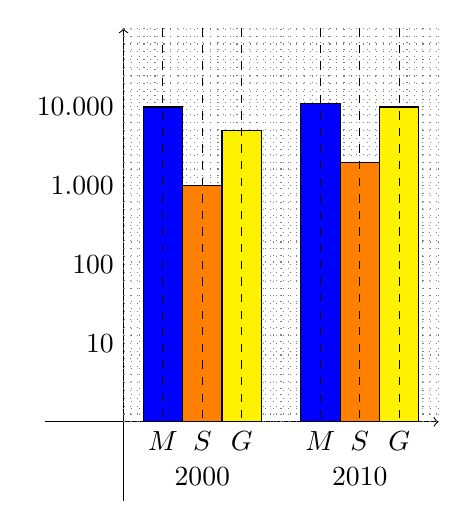
\begin{tikzpicture}[domain=0:5]
\draw[->] (-1,0) -- (4,0);
\draw[->] (0,-1) -- (0,5);
\draw[step=0.1,gray,thin, dotted] (0,0) grid (4,5);
\draw [fill=blue] (0.25,0) rectangle (0.75,4);
\draw [fill=blue] (2.25,0) rectangle (2.75,4.04);
\draw [fill=orange] (0.75,0) rectangle (1.25,3);
\draw [fill=orange] (2.75,0) rectangle (3.25,3.3);
\draw [fill=yellow] (1.25,0) rectangle (1.75,3.7);
\draw [fill=yellow] (3.25,0) rectangle (3.75,4);
\draw[dashed] (1,5) -- (1,0)node[below] {$S$};
\draw[dashed] (1.5,5) -- (1.5,0)node[below] {$G$};
\draw[dashed] (0.5,5) -- (0.5,0)node[below] {$M$};
\node at (1,-0.7) {$2000$};
\node at (3,-0.7) {$2010$};
\draw[dashed] (3,5) -- (3,0)node[below] {$S$};
\draw[dashed] (3.5,5) -- (3.5,0)node[below] {$G$};
\draw[dashed] (2.5,5) -- (2.5,0)node[below] {$M$};
\node[left] at (0,1) {$10$};
\node[left] at (0,2) {$100$};
\node[left] at (0,3) {$1.000$};
\node[left] at (0,4) {$10.000$};
\end{tikzpicture}
\end{center}
\begin{enumerate}
\item A cidade com o maior aumento na população  foi Gotham City, com um acréscimo de 5.000 habitantes.
\item As cidades Smallville e Gotham City dobraram suas populações no período, tendo o mesmo crescimento relativo. A população de Metrópolis aumentou apenas 10\%.
\end{enumerate}}
{1}
\end{resposta}


\begin{ObjetivoEsp}{Para refletir}
{Compreender que gráficos em escala logarítmica apresentam variações iguais para crescimentos relativos iguais.}
{1}
\end{ObjetivoEsp}


\begin{reflection}
No gráfico de escala logarítmica, quais cidades parecem ter sofrido maior alteração em suas populações?
\end{reflection}

\begin{resposta}{Para refletir}
{As cidades de Smallville e Gotham City dobraram suas populações no período e as barras dos gráficos que as representam aumentaram em $\log 2 \approx 0{,}3$. Isso ocorre pois calcular o logaritmo da população vezes um fator é o mesmo que somar o logaritmo daquele fator ao logaritmo da população original. A população da cidade de Metrópolis aumentou o mesmo tanto que a população de Smallville, mas a barra azul quase não se alterou, pois o 1.000 indivíduos equivalem a apenas 10\% da população de Metrópolis no ano 2000, enquanto equivalem a 100\% da população de Smallville no ano 2000.}
{1}
\end{resposta}

\begin{Recomenda}{Crescimento relativo.}
{A taxa de crescimento relativa de uma população é definida como a variação na população em dois momentos distintos dividida pelo tamanho inicial da população. Esse conceito importante na estatística é bem representado em gráficos de escala logarítmica.

Recomenda-se a apresentação da observação "Crescimento proporcional com logaritmos". Ela justifica a interpretação que os gráficos em escala logarítmica representam variações percentuais iguais com a mesma diferença no gráfico, independentemente de suas magnitudes absolutas. Observamos isso nas atividades anteriores, mas poucos exemplos não garantem a validade da propriedade em geral. O cuidado em não assumir generalizações automáticas é uma atitude importante nos processos de argumentação matemática, cuja ênfase é recomendada pela BNCC.}
{1}
\end{Recomenda}

\begin{observation}{Crescimento relativo com logaritmos.}
Se um valor $a$ é acrescido em um percentual $p$ após um determinado período, e outro valor $b$ é acrescido também em $p$ por cento após outro período, então as diferenças entre os logaritmos dos valores (em uma base qualquer $c$, $c\neq 1$) é a mesma:
\begin{align*}
&\log_c (a(1+p))-\log_c a = \log_c ((a(1+p))/a)= \log_c (1+p)\\
&\log_c (b(1+p))-\log_c b = \log_c ((b(1+p))/b)= \log_c (1+p)
\end{align*}

Ou seja, as diferenças (distâncias no gráfico) são as mesmas. Isso significa que \textbf{em um gráfico em escala logarítmica é fácil perceber o crescimento\footnote{Estamos utilizando o termo crescimento relativo mesmo para $c<1$, o que corresponderia a um decrescimento. Todavia o conceito de Taxa de Crescimento Relativo é amplamente utilizado em diversas áreas, mesmo quando o crescimento é negativo (ou seja, há um decrescimento).} proporcional (em relação à magnitude dos valores)}.
\end{observation}

\begin{ObjetivoEsp}{Criptomoedas.}
{\begin{itemize}
\item Comparar dados apresentados em gráficos de escala linear e logarítmica.
\item Utilizar dados de escala logarítmica para compreender a evolução de um investimento.
\end{itemize}}
{1}
\end{ObjetivoEsp}

\begin{Recomenda}{Criptomoedas.}
{O exemplo apresenta os valores de uma Bitcoin, dia a dia, nas escalas linear e logarítmica. Na análise do desempenho de ações ou outros investimentos é comum a utilização de gráficos em escala logarítmica, especialmente para a análise de longo prazo. Recomenda-se que seja ressaltado que o gráfico em escala logarítmica destaca os crescimentos relativos, que eram particularmente difíceis de perceber na escala linear para os dados de menor valor.

Com frequência sites de corretoras trazem a opção de mostrar dados escala logarítmica, o que é uma aplicação fora da matemática para essa técnica.}
{1}
\end{Recomenda}

\begin{example}{Criptomoedas.}
Investidores do mercado financeiro fazem os mais variados tipos de investimentos. Uma forma que têm ganhado popularidade é a compra de criptomoedas, como o Bitcoin. Nesse investimento compram-se unidades da moeda para revenda posterior por um preço maior. O gráfico abaixo ilustra o valor da Bitcoin, dia a dia, no período indicado (dados de coindesk.com).
\begin{center}
\captionof{figure}{Valor de venda de uma Bitcoin (02/10/2013 - 24/05/2020).}\label{bitcoinlinear}
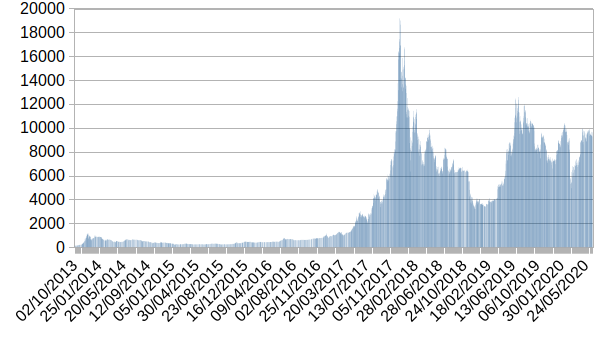
\includegraphics[width=\linewidth]{Bitcoin_linear.png}
\end{center}
Esse gráfico traz informações importantes, mas não é adequado todas as questões. Muitas vezes o investidor está interessado no ganho relativo (crescimento percentual) que a moeda (ou ação) teve e não no valor absoluto da função. Nesse sentido, colocar o gráfico em escala logarítmica ajuda entender os períodos de maior crescimento (ou queda) relativo, devido a observação \textit{Crescimento proporcional com logaritmos}. Vejamos o valor das Bitcoins na escala logarítmica então. 
\begin{center}
\captionof{figure}{Valor de venda de uma Bitcoin (escala logarítmica).}\label{bitcoinlog}
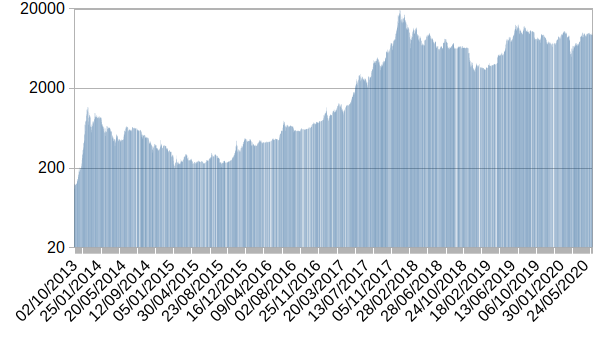
\includegraphics[width=\linewidth]{Bitcoin_log.png}
\end{center}
O gráfico mostra, então, que o crescimento proporcional no início da venda da Bitcoin foi maior do que o crescimento proporcional no pico de valor em dezembro de 2017 / janeiro de 2018, o que não estava aparente no gráfico linear.
\end{example}

\explore{O logaritmo natural}

\begin{ObjetivoEsp}{O logaritmo natural.}
{\begin{itemize}
\item Utilizar logaritmos em base $e$.
\item Aplicar a função logarítmica natural para reescrever funções exponenciais.
\end{itemize}}
{1}
\end{ObjetivoEsp}


\begin{Recomenda}{O logaritmo natural.}
{As funções exponenciais do tipo $f(x) = a e^{kx}$ estão ligada ao crescimento natural pois são as funções cuja taxa de crescimento é proporcional ao valor da função (únicas soluções da equação $df/dx = k f$).  Todavia apresentar esse contexto não está no escopo atual do ensino médio. Por isso apresentamos apenas a informação, sem maiores justificativas.

Os problemas de provas (como ENEM e vestibular) apresentam as questões em diferentes bases, inclusive dentro do mesmo contexto, e isso pode causar confusão. Então apresentamos uma técnica para mudar a base de qualquer exponencial para base $e$ (e que poderia ser utilizada para alterar a base para qualquer outra). Recomenda-se ressaltar que poderíamos escolher a base em que escrevemos as equações de qualquer problema, e que a base $e$ é a base de escolha das ciências naturais.}
{1}
\end{Recomenda}

A função $e^x$, onde $e=2{,}718\cdots$ número de Euler, já foi estudada no capítulo sobre a função exponencial e ela é a função exponencial preferencial nas ciências naturais e na engenharia. Isso ocorre pois ela é a linguagem natural do crescimento. A preferência do logaritmo natural está presente nas próprias calculadoras, que normalmente só calculam logaritmos em base 10, que escrevemos $\log_{10}$ ou $\log$, e a base $e$, que escrevemos $\log_e$ ou $\ln x$.

\begin{observation}{A função logarítmica natural.}
A função logarítmica de base $e$, $\log_e: \mathbb{R}^+_* \to \mathbb{R}$, é chamada de \textbf{função logarítmica natural} e denotada por $\ln$. Assim como para as outras bases, as funções $\ln x$ e $e^x$ são inversas, de modo que, para quaisquer reais $x$ e $y$, com $x>0$, temos:
\begin{align*}
& e^{\ln x} = x;
& \ln e^y = y.
\end{align*}
\end{observation}

Devido a base $e$ expressar o crescimento de forma mais natural, é muito comum que quaisquer exponenciais sejam escritas em termos da função $e^x$ utilizando a seguinte técnica, ilustrada para a função exponencial $5^x$:
$$
5^x = e^{\ln 5^x} = e^{x\ln 5} \approx e^{1{,}609 x},
$$
onde utilizamos a aproximação com três casas decimais para $\ln 5$.

\begin{task}{Na base $e$.}
Escreva as seguintes funções exponenciais utilizando a base $e$, como no exemplo acima, utilizando aproximações com três casas decimais de precisão para os logaritmos naturais.
\begin{enumerate}
\item $f(x)=3^x$;
\item $g(x)=10^x$;
\item $f(x)=75^x$.
\end{enumerate}
\end{task}

\begin{resposta}{Na base $e$.}
{\begin{enumerate}
\item $3^x = e^{\ln 3^x} = e^{x\ln 3} \approx e^{1{,}098 x}$;
\item $10^x = e^{\ln 10^x} = e^{x\ln 10} \approx e^{2{,}302 x}$;
\item $75^x = e^{\ln 75^x} = e^{x\ln 75} \approx e^{4{,}317 x}$.
\end{enumerate}}
{1}
\end{resposta}

\clearmargin

\arrange{Decaimento radioativo}

\begin{ObjetivoEsp}{Decaimento radioativo.}
{Resolver questões contextualizadas envolvendo o contexto de decaimento radioativo.}
{1}
\end{ObjetivoEsp}


\begin{Recomenda}{Decaimento radioativo.}
{Os contextos específicos são importantes no conteúdo de logaritmos, ao ponto de serem explicitados na habilidade EM13MAT305 da BNCC. Por isso dedicamos as últimas seções aos contextos específicos.

Recomenda-se a apresentação dos contextos específicos, pois eles podem parecer difíceis ou estranhos à primeira vista. Todavia destacamos que os contextos apresentados não pretendem substituir o conteúdo das respectivas matérias (física, biologia, química, ...), mas complementá-lo.

O estudo do decaimento radioativo abre a oportunidade para o estudo interdisciplinar da radiação com a física ou da datação por Carbono-14 com a química ou a biologia.}
{1}
\end{Recomenda}

\begin{center}
\begin{tikzpicture}
    % Carbono
    \coordinate (dv) at (0,0);
    \coordinate (base) at (50pt,0pt);
    \coordinate (height) at (0pt,50pt);
    \coordinate (diag) at ($(base)+(height)$);
    \fill[rounded corners=2pt, grafite] ($(dv)-.5*(diag)$) rectangle +(diag); 
    \node[white] at (dv) {\sffamily\Huge \textbf{C}};
    \node[white, inner sep=2pt] (dvtext) at ($(dv)-.5*(height)$) [anchor=south] {\sffamily\small Carbono};
    \node[white, inner sep=2pt] (dvnum) at ($(dv)+.5*(height)-.5*(base)$) [anchor=north west] {\sffamily\small 6};
    \node[white, inner sep=2pt] (dvnum) at ($(dv)+.5*(height)+.5*(base)$) [anchor=north east] {\sffamily\small 12};
\end{tikzpicture}
\end{center}

Os elementos químicos são catalogados na tabela periódica. A figura acima ilustra o \textbf{isótopo mais comum do carbono}, o Carbono-12, que tem número atômico 6 (e, assim, 6 prótons) e número de massa 12, tendo 6 nêutrons. Contudo nem todos os átomos de carbono são iguais, alguns têm nêutrons em excesso ou em falta. Classificamos os átomos em isótopos de acordo com o número de nêutrons que eles têm. Um isótopo importante do carbono é o Carbono-14, que é utilizado na datação de objetos antigos.

O Carbono-14 é um isótopo instável, e pode, espontaneamente, emitir radiação (e transformar-se em um átomo de nitrogênio). Esse processo natural é chamado de decaimento radioativo e diferentes isótopos decaem à taxas (velocidades) diferentes.

\begin{observation}{A meia vida de isótopos radioativos.}
A \textbf{meia vida} de um isótopo radioativo é o tempo necessário para que a metade dos átomos daquele isótopo em uma amostra decaia. Alguns exemplos de meia-vida de isótopos:
\begin{center}
\begin{tabular}{|l|r|}
\hline
\cellcolor[HTML]{00A59D} Oxigênio-19 & 26,5 s\\
\hline
\cellcolor[HTML]{00A59D} Césio-137 & 30 anos\\
\hline
\cellcolor[HTML]{00A59D} Carbono-14 & 5730 anos \\
\hline
\cellcolor[HTML]{00A59D} Urânio-235 & 703.800.000 anos\\
\hline
\end{tabular}
\end{center}
\captionof{table}{Meias-vidas de alguns isótopos radioativos (aproximações).}
\end{observation}

\begin{example}{Decaimento do Carbono-14.}
O decaimento do Carbono-14 é utilizado para determinar a idade de tecidos orgânicos mortos e, por isso, é muito importante em diversas áreas da ciência. Vamos considerar uma amostra com 100g de Carbono-14 e determinar quanto tempo seria necessário para que sobrasse apenas 10g de Carbono-14 na amostra.

Como perdemos metade da massa a cada meia-vida, teremos as seguintes quantidades de Carbono-14 após determinado número de anos
\begin{center}
\begin{tabular}{|l|l|l|l|l|l|l|}
\hline
\cellcolor[HTML]{00A59D} Anos & 0 & 5.730 & 11.460 & 17.190 & 22.920 & 28.650\\
\hline
\cellcolor[HTML]{00A59D} Carbono-14 & 100g & 50g & 25g & 12,5g & 6,25g & 3,125g
\\
\hline
\end{tabular}
\end{center}
\captionof{table}{Quantidade de Carbono-14 restante.}

Vemos que a quantidade cai exponencialmente a cada 5.730 anos. Assim, poderíamos escrever uma expressão para a quantidade de Carbono-14 como
$$
Q(t) = 100\times \left(\frac{1}{2}\right)^{t/5730} = 100\times e^{t\frac{\ln 1/2}{5730}} = 100\times e^{-t\frac{0{,}693}{5730}},
$$
onde escrevemos a função exponencial de base $e$ por ser a mais utilizada nesse contexto. Assim o tempo necessário para termos 10g seria
\begin{align*}
& 0{,}1=e^{-t\frac{0{,}693}{5730}}\\
\Longrightarrow& -t\frac{0{,}693}{5730} = \ln 0{,}1\\
\Longrightarrow& t \approx \frac{5730}{0{,}693}2,302 = 19.033{,}852
\end{align*}
\end{example}

\begin{Recomenda}{Meia vida biológica.}
{Na farmácia e na medicina utiliza-se a meia vida como meio para aproximar a concentração plasmática de um fármaco em um organismo após a administração. A resolução da questão é análoga às resoluções envolvendo o decaimento radioativo e a adaptação das técnicas conhecidas entre contextos diferentes é fundamental, uma vez que a exploração de todos os contextos específicos possíveis não é viável.}
{1}
\end{Recomenda}

\begin{task}{Meia vida biológica.}
A meia vida de um fármaco é o tempo necessário para a concentração plasmática dele cair pela metade em um organismo. Esse conceito serve para estimarmos qual a concentração de determinado medicamento no organismo. O antibiótico Amoxicilina tem meia vida biológica de 61,3 minutos. Vejamos a seguinte situação: um paciente de 75Kg recebe uma dose do medicamento de 500mg. Uma pessoa com esse peso tem cerca de 5 litros de sangue (a quantidade exata pode variar de pessoa para pessoa). Supondo que o medicamento foi completamente dissolvido e distribuído uniformemente no sangue, teríamos a concentração plasmática do medicamento igual a 500/5000 = 0,1 mg/ml. Escreva uma função exponencial de base $e$ para descrever concentração plasmática (em mg/ml) após $t$ minutos. Utilize a função encontrada para determinar quanto tempo levará para a concentração cair abaixo de 0,005 mg/ml. 
\end{task}

\begin{resposta}{Meia vida biológica.}
{Como a concentração cai pela metade a cada 61,3 minutos, poderíamos escrever a seguinte função para a concentração
$$
Q(t)=0{,}1(1/2)^{t/61{,}3},
$$
que pode ser escrita na base $e$ como
\begin{align*}
Q(t)=&0{,}1e^{(t/61{,}3)\ln{(1/2)}}\\
\approx &0{,}1e^{-t\frac{0{,}693}{61{,}3}} = 0{,}1e^{-0{,}0113t}.
\end{align*}
Assim o tempo necessário para a concentração cair abaixo de 0,005 pode ser calculado resolvendo:
\begin{align*}
&0{,}005 = 0{,}1e^{-0{,}0113t}\\
\Rightarrow &e^{-0{,}0113t} = 0{,}05\\
\Rightarrow &t = \frac{-\ln 0{,}05}{0{,}0113} \approx 265{,}1.
\end{align*}
E seria necessário mais de 265min e 10s para a concentração cair abaixo de 0,005 mg/ml.}
{1}
\end{resposta}


\explore{Escalas logarítmicas.}

\section{Escala Richter}

\begin{Recomenda}{Escala Richter}
{A utilização da escala Richter para a determinação da magnitude de  eventos sísmicos de larga escala não é mais feita hoje em dia. Todavia ela é tão famosa que, muitas vezes, magnitudes em outras escalas são atribuídas a ela e questões de provas ainda fazem referência a ela.

Ressaltamos, ainda, que não usa-se \textit{graus} na escala Richter. Uma escala em graus é a de Mercalli, que avalia os danos causados às estruturas locais, todavia ela não é diretamente correlacionada à magnitude (física) do evento.}
{1}
\end{Recomenda}

Ocorrem milhares de eventos sísmicos todo o dia no planeta Terra, mas a grande maioria deles é muito fraca para ser percebida pelos seres humanos. A magnitude de um evento sísmico varia muito, por isso tais eventos são classificados em escalas logarítmicas. Uma escala bastante famosa para medir os abalos é a escala Richter (mas que não é tão utilizada hoje em dia).

A escala Richter\footnote{Desenvolvida por Charles Richter e Beno Gutenberg} utiliza as amplitudes da das ondas registradas por sismógrafos para expressar a magnitude local de um evento sísmico, onde está localizado o sismógrafo.
\begin{figure}[!h]
\centering
\caption{Um sismógrafo e o registro de um evento}
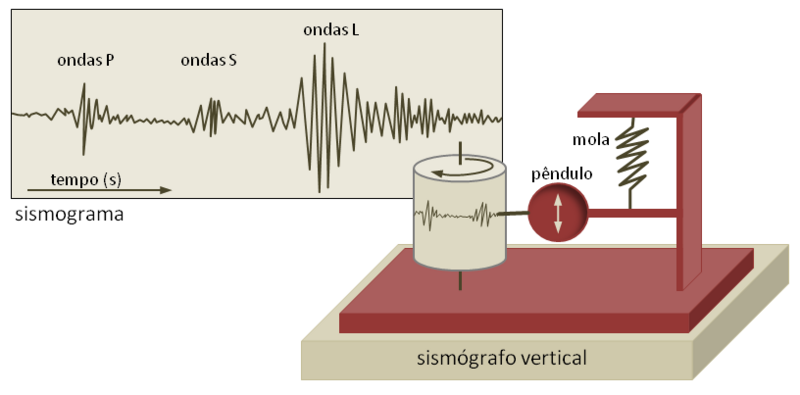
\includegraphics[width=0.8\linewidth]{Sismografo.png}\\
\textbf{Fonte:} Casa das Ciências (https://www.casadasciencias.org/).
\end{figure}

A Magnitude Local (ML) determinada pela escala Richter pode ser calculada por
$$
ML = \log_{10} A - \log A_0,
$$
onde $A$ é a maior amplitude de onda detectada pelo sismógrafo e $A_0$ é a magnitude do menor abalo registrável (na época de sua invenção), corrigida por um fator de escala, que depende da distância do sismógrafo à fonte do tremor.


\begin{example}{Comparando eventos (Escala Richter).}
Segundo a Wikipedia, a explosão na central nuclear de Chernobyl, em 1986, apresentou Magnitude Local $ML_{Ch} = 3{,}67$, enquanto o Sismo da Costa Rica, em 2009, apresentou Magnitude Local de $ML_{CR}=6{,}2$. Podemos comparar os eventos calculando a razão entre as amplitudes registradas através da diferença entre as Magnitudes Locais:
\begin{align*}
&6{,}2-3{,}67 = \log_{10} A_{CR} - \log A_0 - (\log_{10} A_{Ch} - \log A_0)\\
\Rightarrow & 2{,}53 = \log_{10} A_{CR} - \log_{10} A_{Ch} = \log_{10} \left(\frac{A_{CR}}{A_{Ch}}\right)\\
\Rightarrow & \left(\frac{A_{CR}}{A_{Ch}}\right) = 10^{2{,}53} \approx 338{,}84.
\end{align*} 
Assim o Sismo da Costa Rica registrou amplitudes 338 vezes maiores do que a explosão nuclear de Chernobyl.
\end{example}

A escala Richter apresenta distorções para eventos de grande ($>6{,}5$) intensidade e não é utilizada para grandes eventos sísmicos atualmente.

\section{Magnitude de Momento Sísmico}

\begin{Recomenda}{Magnitude de Momento Sísmico}
{A escala de Magnitude de Momento Sísmico é a escala mais utilizada para eventos de grande magnitude atualmente.}
{1}
\end{Recomenda}

Uma escala bastante utilizada atualmente é a escala de Magnitude ds Momento Sísmico ($MMS$), que também é uma escala logarítmica e utiliza o Momento Sísmico ($M_0$) para estimar a magnitude de um evento através da equação
$$
M_{\mathrm {w} }={2 \over 3}\log_{10}\left(M_{0}\right)-10,7
$$

\begin{example}{Comparando eventos (MMS).}
Segundo a Wikipedia, a explosão da Tsar Bomba (maior artefato nuclear já detonado), detonada em 1961, atingiu Magnitude de Momento Sísmico $M_{\mathrm w} = 8{,}3$, enquanto o impacto do meteoro que, presumidamente, causou a extinção dos dinossauros, atingiu Magnitude de Momento Sísmico $N_{\mathrm w} = 13{,}0$. Podemos comparar os eventos calculando a razão entre os Momentos Sísmicos $M_T$ e $M_D$, respectivamente, calculando a diferença entre as Magnitudes de Momento Sísmicos:
\begin{align*}
&13{,}0-8{,}3 = {2 \over 3}\log_{10}\left(M_{D}\right)-10,7-\left( {2 \over 3}\log_{10}\left(M_{T}\right)-10,7\right)\\
\Rightarrow & 4{,}7 = {2 \over 3}\left(\log_{10}\left(M_{D}\right)-\log_{10}\left(M_{T}\right)\right) =  {2 \over 3}\log_{10}\left(\frac{M_D}{M_T}\right)\\
\Rightarrow & \left(\frac{M_D}{M_T}\right) = 10^{7{,}05} \approx 11.220.184{,}54.
\end{align*} 
Assim o impacto do meteoro gerou um Momento Sísmico mais de 11 milhões de vezes maior do que o Momento Sísmico do maior artefato nuclear já detonado pela espécie humana. 
\end{example}

\section{pH}

\begin{Recomenda}{pH}
{O estudo do pH abre a oportunidade para o estudo interdisciplinar do assunto na química. Isso é particularmente recomendado pois o cálculo pode ser realizado de forma diferente em outros contextos.}
{1}
\end{Recomenda}

O pH, às vezes chamado de potencial de Ionização, é uma escala utilizada para medir a acidez ou basicidade de uma solução aquosa. Substâncias ácidas tem o pH menor do que 7 e substâncias básica tem o pH maior do que 7. A água pura tem pH=7 e é considerada neutra. Vejamos alguns exemplos dos valores de pH  para substâncias comuns:

\begin{center}
\captionof{table}{Alguns valores comuns de pH.}
\begin{tabular}{|l|l|}
\hline
\cellcolor[HTML]{00A59D} Substância &	\cellcolor[HTML]{00A59D} pH\\
\hline
Ácido de bateria & < 1,0\\
\hline
Suco gástrico	& 1,0 - 3,0\\
\hline
Sumo de limão	& 2,2 - 2,4\\
\hline
Refrigerante tipo cola	& 2,5\\
\hline
Vinagre	& 2,4-3,4\\
\hline
Sumo de laranja ou maçã	& 3,5\\
\hline
Cervejas	& 4,0 - 5,0\\
\hline
Café	& 5,0\\
\hline
Chá &	5,5\\
\hline
Chuva ácida	& < 5,6\\
\hline
Leite	& 6,3 - 6,6\\
\hline
Água pura	&7,0\\
\hline 
Saliva humana	& 6,5 - 7,5\\
\hline
Sangue humano	& 7,35 - 7,45\\
\hline
Água do mar	& 8,0\\
\hline 
Sabonete de mão	& 9,0 - 10,0\\
\hline
Amoníaco &	11,5\\
\hline
Hidróxido de sódio (soda cáustica)&	13,5\\
\hline
\end{tabular}\\
\vspace{3mm}
\textbf{Fonte:} dados da Wikipedia-pH (pt.wikipedia.org/wiki/PH).
\end{center}

O pH é definido a partir da atividade dos íons de hidrônio ($a_{H^+}$), medida em mols/L, na solução, que pode ser medida com um aparelho eletrônico. Então o pH é definido como menos o logaritmo da atividade dos íons de hidrônio:
$$
pH = - \log_{10} a_{H^+}
$$

\begin{resposta}{pH no vestibular.}
{A chuva ácida tem pH 1 unidade menor do que o pH da chuva comum. Isso indica que a atividade de íons de hidrônio é 10 vezes maior. Assim a chuva ácida é dez vezes mais ácida.}
{1} 
\end{resposta}

\begin{task}{\,pH no vestibular.}
[UDESC 2009] “Chuva ácida” é um termo que se refere à precipitação, a partir da
atmosfera, de chuva com quantidades de ácidos nítricos e sulfúrico maiores que o
normal. Os precursores da chuva ácida vem tanto de fontes naturais, tais como vulcões
e vegetação em decomposição, quanto de processos industriais, principalmente
emissões de dióxido de enxofre e óxidos de nitrogênio resultantes da queima de
combustíveis fósseis. O pH da água da chuva considerado normal é de 5,5 (devido
à presença de ácido carbônico proveniente da solubilização de dióxido de carbono).
Um químico monitorando uma região altamente industrializada observou que o pH da
água da chuva era igual a 4,5. Considerando que a acidez está relacionada com a
concentração de $H_3O^+$, é correto afirmar que a água com pH 4,5 era:
\begin{itemize}
\item[(A)] duas vezes mais básica que o normal.
\item[(B)] duas vezes mais ácida que o normal.
\item[(C)] dez vezes mais básica que o normal.
\item[(D)] dez vezes mais ácida que o normal.
\item[(E)] cem vezes mais ácida que o normal.
\end{itemize}
\end{task}



\exercise

\begin{resposta}{Exercício \ref{Exer1}}
{A formiga aparenta ter massa de $10^{-6}$Kg e o besouro parece ter massa de cerca de $10^{-4}$Kg, assim o peso do besouro é cerca de 100 vezes o peso da formiga. Já o coelho, com $1$Kg, tem 10.000 vezes o peso do besouro e 1.000.000 de vezes o peso da formiga.}
{1}
\end{resposta}

\clearmargin

\begin{resposta}{Exercício \ref{Exer2}}
{O gráfico em escala linear não permite entender a evolução dos dados quando a magnitude deles é muito pequena em relação ao número total de casos. No gráfico em escala logarítmica, que preserva os crescimentos relativos, vê-se que no intervalo inicial o número de casos aumenta mais de 10 vezes, mas muito menos do que isso entre 30 de abril e 20 de maio. O gráfico em escala logarítmica é melhor para observarmos variações em dados que tenham natureza exponencial. Por exemplo percebe-se uma redução na taxa de crescimento no início de março, mas uma nova aceleração no final do mês.}
{1}
\end{resposta}

\clearmargin

\begin{resposta}{Exercício \ref{Exer3}}
{O gráfico em escala linear não permite entender a evolução dos dados quando a magnitude deles é muito pequena em relação ao número total de casos. No gráfico em escala logarítmica, que preserva os crescimentos relativos, vê-se um crescimento mais acentuado entre 02/10/2013 e 25/01/2014 do que entre 05/11/2017 e 28/02/2018. O pico de valor nas Bitcoins em escala linear acaba mascarando outros períodos de crescimento relativo (percentual) similares em outros períodos, nos quais o valor absoluto da moeda era menor.}
{1}
\end{resposta}

\begin{resposta}{Exercício \ref{Exer4}}
{O número de dias necessários para a planta atingir sua altura de venda pode ser encontrada resolvendo a equação
\begin{align*}
&30 = 5\log_2 (t+1)\\
\Rightarrow &t+1 = 2^6\\
\Rightarrow &t = 63.
\end{align*}
O número de dias necessários para a planta atingir sua altura máxima pode ser encontrado resolvendo a equação
\begin{align*}
&40 = 5\log_2 (t+1)\\
\Rightarrow& t+1 = 2^8\\
\Rightarrow& t = 255.
\end{align*}
Assim entre os dois períodos temos $255-63 = 192$ dias.}
{1}
\end{resposta}

\clearmargin

\begin{resposta}{Exercício \ref{Exer5}}
{Podemos encontrar o tempo necessário resolvendo a equação
\begin{align*}
&50 = 5(1{,}184)^t\\
\Rightarrow& (1{,}184)^t = 10\\
\Rightarrow& t\log(1{,}184) = 1\\
\Rightarrow& t = \frac{1}{0{,}073} \approx 13{,}
7.
\end{align*}
Assim seria necessário mais do que 13 anos e teríamos 50 milhões de usuários entre 2013 e 2014.}
{1}
\end{resposta}

\begin{resposta}{Exercício \ref{Exer6}}
{$pH = -\log 10^{-5}=5$.}
{1}
\end{resposta}

\begin{resposta}{Exercício \ref{Exer7}}
{Apenas as proposições II e III são verdadeiras pois:

I - É falsa pois nenhuma das informações dadas permite calcular o valor de $A_0$.

II- \hspace{30mm}\begin{minipage}[t]{0.8\linewidth}
$\,\,\,\,\,\,\,4 = \log (A) - \log (A_0)$

$\Rightarrow 4 = \log (A/A_0)$

$\Rightarrow (A/A_0) = 10^4.$
\end{minipage}

III- \begin{minipage}[t]{0.8\linewidth}
Se a amplitude do primeiro terremoto é $A_1$ e a amplitude do segundo terremoto é $A_2$, temos
\begin{align*}
&1 = \log (A_1) - \log (A_0)\\
& \hspace{4mm}- (\log (A_2) - \log (A_0))\\
\Rightarrow &1 = \log (A_1/A_2)\\
\Rightarrow &(A_1/A_2) = 10.
\end{align*}
\end{minipage}}
{1}
\end{resposta}

\begin{resposta}{Exercício \ref{Exer8}}
{Aplicando os valores na expressão
\begin{align*}
&7{,}3 = -10{,}7+\frac{2}{3} \log M_0\\
\Rightarrow & \frac{2}{3} \log M_0 = 18\\
\Rightarrow & \log M_0 = 27\\
\Rightarrow & M_0 = 10^{27}.
\end{align*}}
{1}
\end{resposta}

\clearmargin

\begin{resposta}{Exercício \ref{Exer9}}
{O tempo pode ser encontrado resolvendo
\begin{align*}
&3{,}5 = 1{,}5+\log_3 (t+1)\\
\Rightarrow & \log_3 (t+1) = 2\\
\Rightarrow & (t+1) = 3^2 =9\\
\Rightarrow & t = 8.
\end{align*}}
{1}
\end{resposta}

\begin{resposta}{Exercício \ref{Exer10}}
{Podemos encontrar o tempo necessário resolvendo a equação
\begin{align*}
& 30 = 5(1{,}02)^t\\
\Rightarrow & (1{,}02)^t = 6\\
\Rightarrow & t\ln(1{,}02) = \ln 2 + \ln 3\\
\Rightarrow & t \approx \frac{0{,}7+1{,}1}{0{,}02}=90.
\end{align*}
Seriam necessários 90 anos se a taxa de crescimento permanecesse a mesma (contudo não há evidências para essa suposição).}
{1}
\end{resposta}

\begin{resposta}{Exercício \ref{Exer11}}
{Calcula-se o pH diretamente da fórmula:
\begin{align*}
pH =& -\log (5{,}4\times 10^{-8})\\
=& -\log (3^3\times 2 \times 10^{-9})\\
\approx& 9-3\log 3 -\log 2 \\
\approx& 9 -3\times 0{,}48 -0{,}3=7{,}26.
\end{align*}}
{1}
\end{resposta}

\begin{resposta}{Exercício \ref{Exer12}}
{A temperatura $T$, em $^oC$, pode ser escrita em função do tempo $t$, em minutos, através da expressão:
$$
T(t) = 3000(0{,}99)^{t/30}.
$$
Calcula-se o pH diretamente da fórmula:
\begin{align*}
&30= 3000(0{,}99)^{t/30}\\
\Rightarrow & 1/100 = (0{,}99)^{t/30}\\
\Rightarrow & \frac{t}{30} \log(0{,}99)= -2\\
\Rightarrow & t= -\frac{60}{\log(0{,}99)} \\
&\,\,= -\frac{60}{-2+\log(3^2)+\log(11)}\\
&\,\,\approx \frac{60}{0{,}005} = 12000.
\end{align*}
Assim serão necessários 12000min=200h.}
{1}
\end{resposta}

\begin{resposta}{Exercício \ref{Exer13}}
{Podemos encontrar o tempo necessário resolvendo a equação
\begin{align*}
& \frac{P_0}{4} = P_0 e^{-\frac{t}{250}}\\
\Rightarrow & e^{-\frac{t}{250}} = \frac{1}{4}\\
\Rightarrow & -\frac{t}{250} = \ln \left(\frac{1}{4}\right) \approx -2 \times 0{,}693\\
\Rightarrow & t \approx 250 \times 2 \times 0{,}693 = 346{,}5.
\end{align*}
Seriam necessários aproximadamente 346 dias.}
{1}
\end{resposta}

\begin{resposta}{Exercício \ref{Exer14}}
{Podemos encontrar a altitude diretamente da equação
\begin{align*}
 h =& 20 \log 1/0{,}4 = 20 \log 10/4\\
=& 20 (\log 10 -2\log 2)\\
\approx& 20 (1-2\times0,3) = 8.
\end{align*}
Assim a altitude é de 8Km.}
{1}
\end{resposta}

\begin{resposta}{Exercício \ref{Exer15}}
{A probabilidade de ganhar ao menos um partida, dentre $n$ jogadas, pode ser calculada como 1 menos a probabilidade de perder todas consecutivamente
\begin{align*}
P =& 1 - 0{,}9^n.
\end{align*}
Assim, o número de partidas necessário para que a probabilidade de vencer ao menos uma seja maior do que 99\% pode ser obtida resolvendo
\begin{align*}
 &0{,}99 = 1 - 0{,}9^n\\
\Rightarrow & 0{,}9^n = 0{,}01\\
\Rightarrow & n\log(0{,}9) = \log(0{,}01)\\
\Rightarrow & n = \frac{-2}{\log(9/10)}= \frac{-2}{2\log(3)-1}\\
& \,\, \approx\frac{-2}{-0{,}046} \approx 43{,}48.
\end{align*}
Contudo o número de partidas só pode ser um número inteiro positivo, desse modo serão necessárias 44 partidas para que a probabilidade de que haja vitória em apenas uma delas seja maior do que 99\%.}
{1}
\end{resposta}

\begin{enumerate}


\item \label{Exer1} Segundo o gráfico abaixo, quantas vezes a massa corporal de um besouro é maior do que a massa corporal de uma formiga? E qual seria a razão entre as massas de um coelho e de um besouro? E entre as massas da formiga e do coelho?
\begin{center}
\captionof{figure}{Distribuição de massas, em quilogramas no eixo horizontal, e velocidades, em comprimentos do ser vivo por segundo no eixo horizontal.}
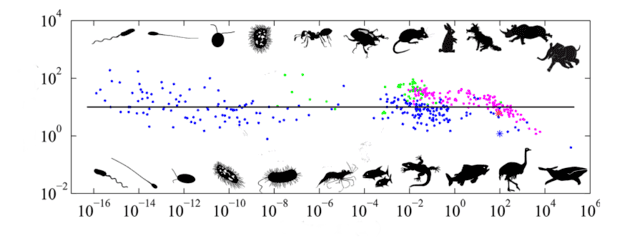
\includegraphics[width=\linewidth]{Massa.png}\vspace{3mm}\\
\textbf{Fonte:} \cite{Mayer15}.%;  https://doi.org/10.1119/1.4917310 - Nicole Meyer-Verneta.
\end{center}

\item \label{Exer2} Para doenças infecciosas, em seus estágios iniciais, é esperado que o aumento no número de casos seja proporcional ao número de contaminados (em estágios posteriores essa tendência diminuí pois há menos pessoas suscetíveis disponíveis para a contaminação). Os gráficos abaixo mostram o desenvolvimento  do número de casos da Covid-19 no mundo em escala linear e logarítmica. Observando os gráficos, houve maior crescimento relativo no número de casos entre as datas de 22 de janeiro e 10 de fevereiro ou entre as datas de 30 de abril e 20 de maio? Qual dos gráficos identifica melhor a situação?
\begin{center}
\captionof{figure}{Total de casos confirmados da Covid-19 no mundo (linear).}
\includegraphics[width=\linewidth]{World_linear.png}\vspace{3mm}\\
\textbf{Fonte:} Our World in Data (ourworldindata.org).
\end{center}
\begin{center}
\captionof{figure}{Total de casos confirmados da Covid-19 no mundo (log).}
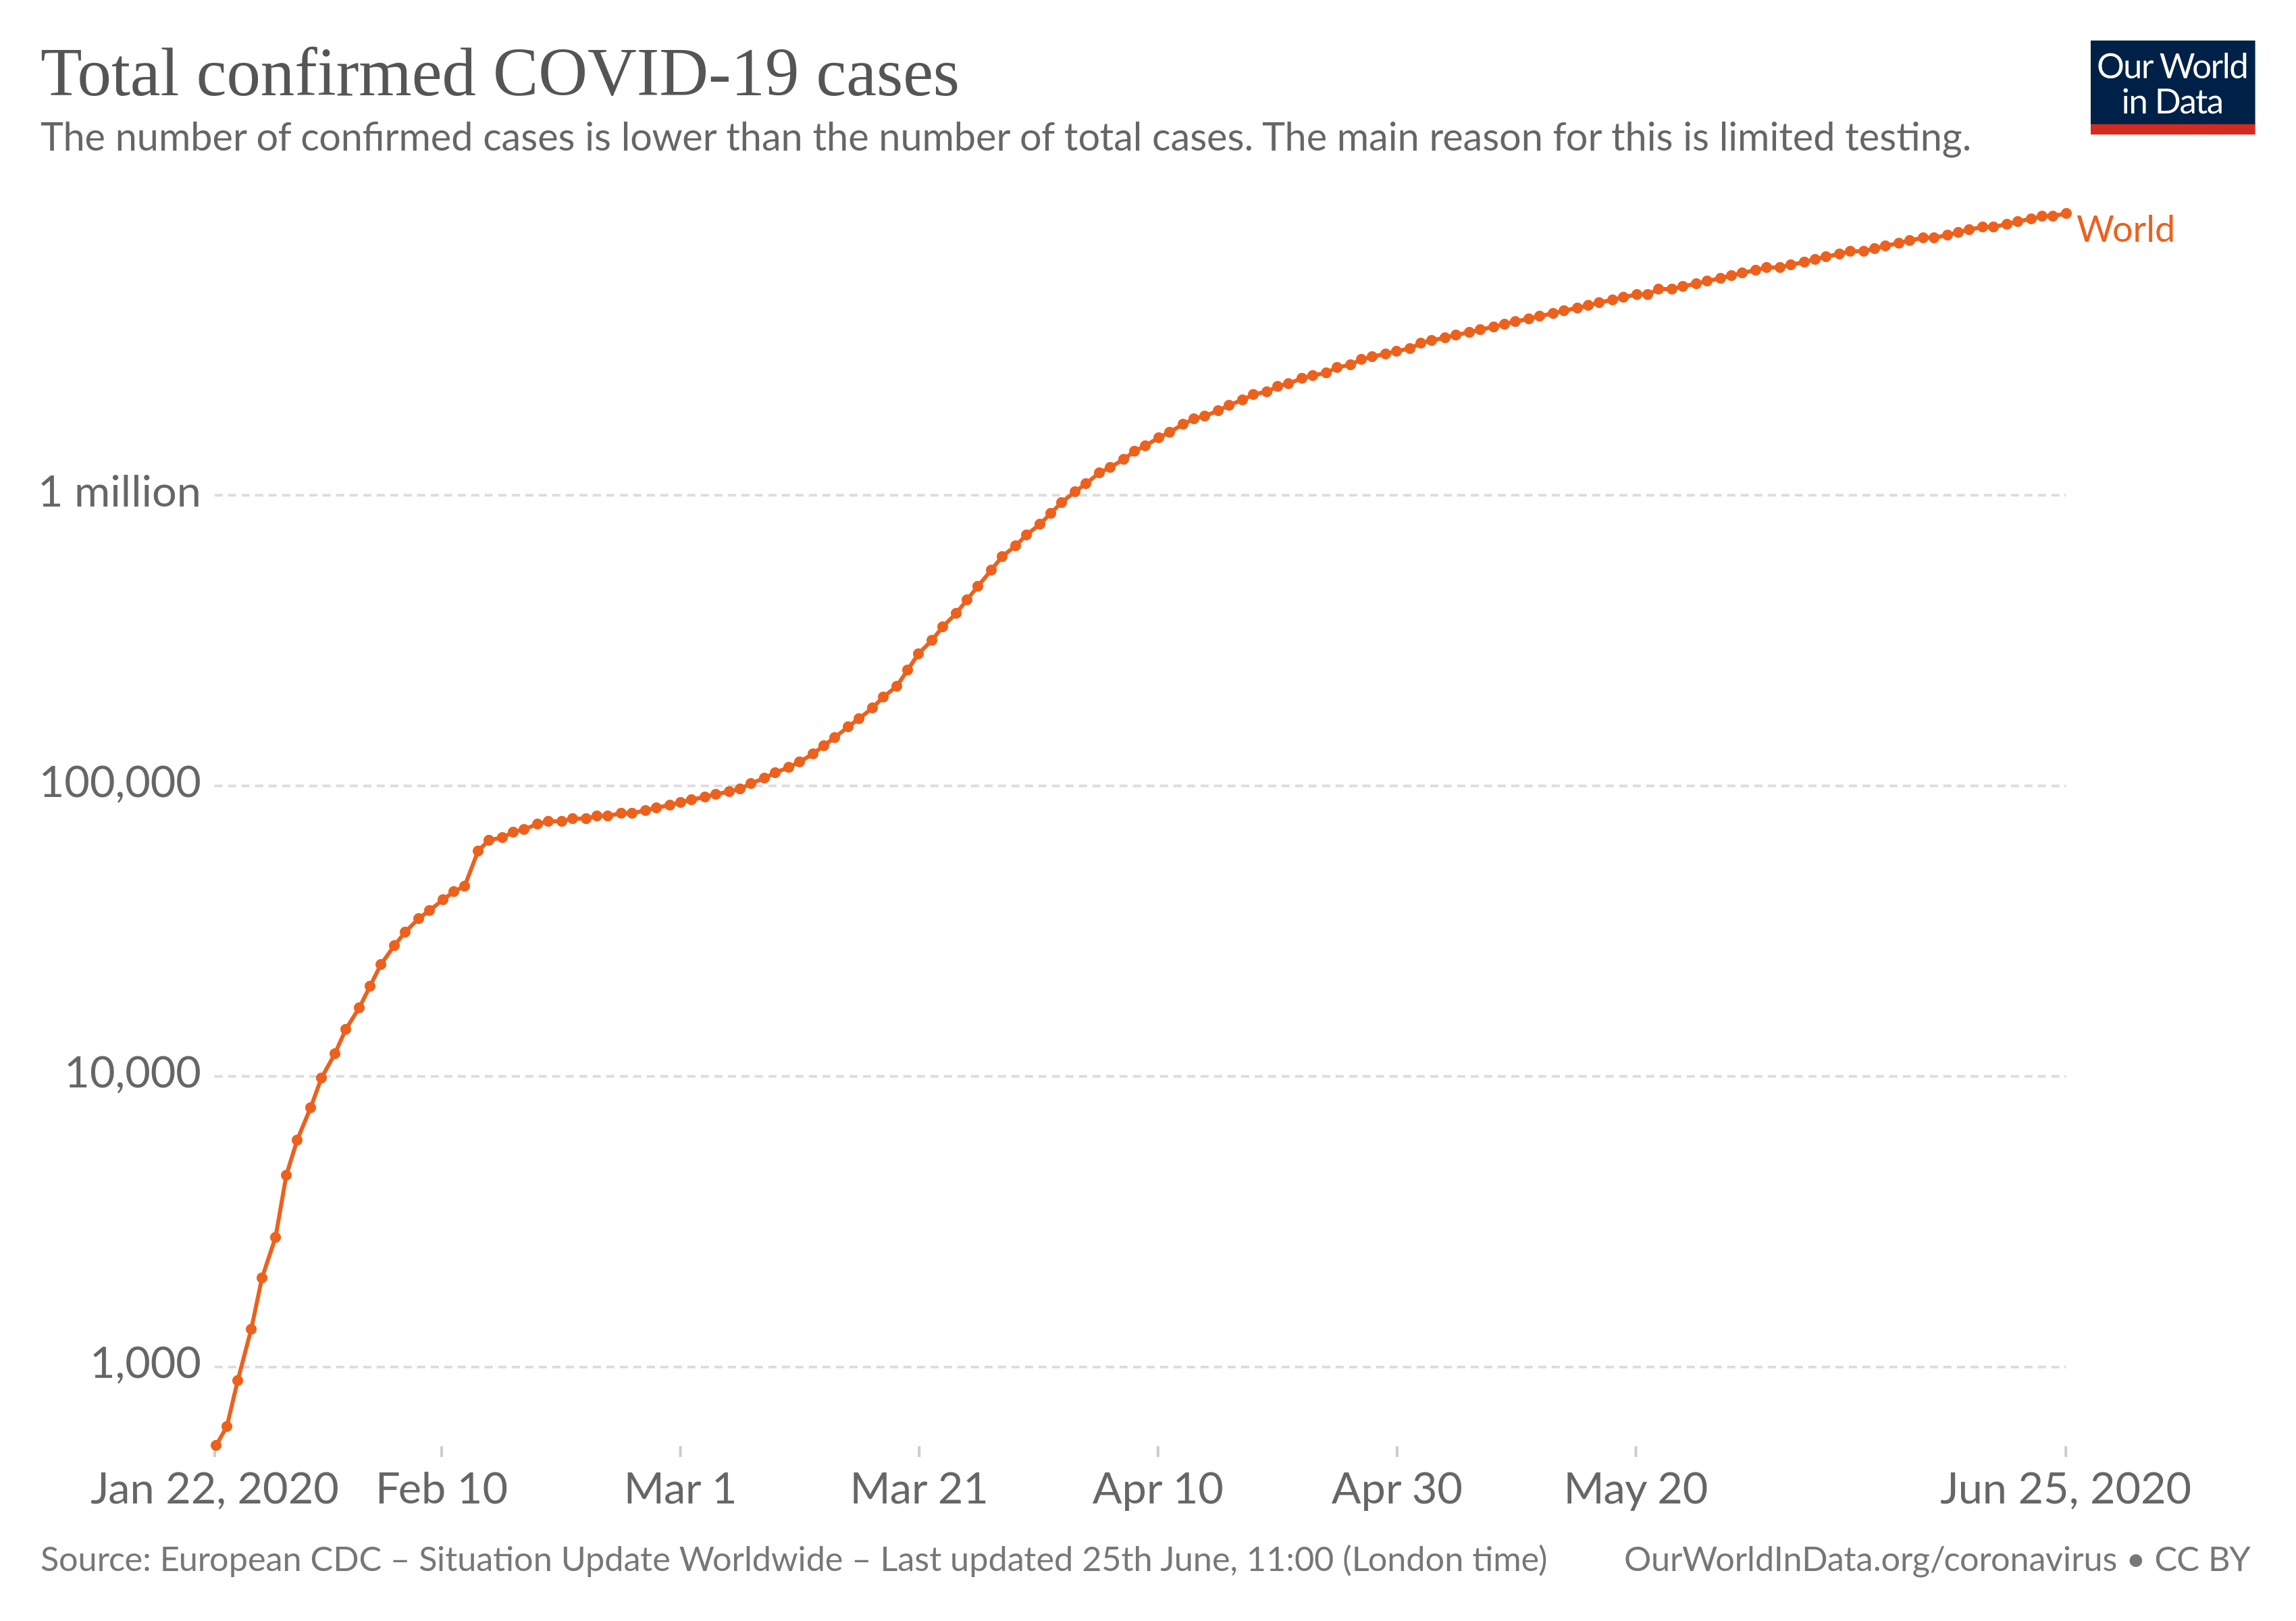
\includegraphics[width=\linewidth]{World_log.png}\vspace{3mm}\\
\textbf{Fonte:} Our World in Data (ourworldindata.org).
\end{center}

\item \label{Exer3} Observando as figuras \ref{bitcoinlinear} e \ref{bitcoinlog}, o crescimento percentual do valor da Bitcoin foi maior entre as datas de 02/10/2013 e 25/01/2014 ou entre 05/11/2017 e 28/02/2018? Como isso pode ser observado nos gráficos?


\item \label{Exer4} (ENEM 2019) Um jardineiro cultiva plantas ornamentais e as coloca à venda quando estas atingem 30 centímetros de altura. Esse jardineiro estudou o crescimento de suas plantas, em função do tempo, e deduziu uma fórmula que calcula a altura em função do tempo, a partir do momento em que a planta brota do solo até o momento em que ela atinge sua altura máxima de 40 centímetros. A fórmula é $h = 5\log_2 (t + 1)$, em que t é o tempo contado em dia e h, a altura da planta em centímetro. A partir do momento em que uma dessas plantas é colocada à venda, em quanto tempo, em dia, ela alcançará sua altura máxima?
\begin{enumerate}
\item 63
\item 96
\item 128
\item 192
\item 255
\end{enumerate}


\item \label{Exer5} (PEIES/2008) Segundo o IBOPE, o número de internautas no Brasil chegou, em março de 2007, a 16,3 milhões de pessoas. Em 2000, esse número era aproximadamente 5 milhões. Suponha que a função N(t), que representa o número de internautas\footnote{Em uma situação real, só é possível esperar crescimento exponencial enquanto o total de internautas é muito menor do que a população total.} (em milhões) em função do tempo $t$ (em ano), possa ser expressa por $N(t) = 5(1{,}184)^t$, onde $t = 0$ representa o ano de 2000, $t = 1$, o ano de 2001 e assim por diante. Então, de acordo com esse modelo, o número de internautas atingirá 50 milhões: (dado $\log 1{,}184 = 0{,}073$)
\begin{enumerate}
\item entre 2008 e 2009;
\item entre 2009 e 2010;
\item em março de 2010;
\item entre 2013 e 2014;
\item somente a partir de 2015.
\end{enumerate}



\item \label{Exer6}

O pH de uma solução é definido por pH$=-\log_{10}(H^+)$  em que $H^+$ é a concentração de hidrogênio em íons-grama por litro de solução. Determine o pH de uma solução tal que $H^+ = 10^{-5}$.


   
\item \label{Exer7} (USF Geral 2015) Terremoto é o termo popular usado para os grandes sismos, sendo que para os pequenos é comum 
usar 
abalo sísmico ou tremor de terra. A escala Richter, também conhecida como escala de magnitude local (ML), atribui um 
número único para quantificar o nível de energia liberada por um sismo. É uma escala logarítmica de base 10, obtida 
calculando o logaritmo da amplitude horizontal combinada (amplitude sísmica) do maior deslocamento a partir do zero em 
um tipo particular de sismógrafo. 

A fórmula utilizada é $ML = \log(A) - \log (A_0)$, em que: 

A = amplitude máxima medida no sismógrafo. 

$A_0$ = uma amplitude de referência. 

Com base nas informações, analise as proposições: 

I. Para um terremoto de magnitude 7, temos que $A_0 = 7A$. 

II. Para um terremoto de magnitude 4 temos que $\frac{A}{A_0}=10^{-4}$ .
 
III. Um terremoto de magnitude 7 produz efeitos 10 vezes maior do que um terremoto de magnitude 6. 

Assinale a correta.
\begin{enumerate}
    \item Apenas a proposição I é verdadeira.
    \item Apenas as proposições I e II são verdadeiras
	\item Apenas as proposições II e III são verdadeiras.
	\item Apenas a proposição II é verdadeira.
	\item Apenas a proposição III é verdadeira.
\end{enumerate}


\item \label{Exer8} (Enem 2011) A Escala de Magnitude de Momento (abreviada como MMS e denotada como $M_w$), introduzida em 1979 por Thomas 
Haks e Hiroo Kanamori, substituiu a Escala de Richter para medir a magnitude dos terremotos em termos de energia 
liberada. Menos conhecida pelo público, a MMS é, no entanto, a escala usada para estimar as magnitudes de todos os 
grandes terremotos da atualidade. Assim como a escala Richter, a MMS é uma escala logarítmica. 
$M_w$ e $M_0$ se relacionam pela fórmula:
$$
M_w = - 10,7 + \frac{2}{3}\log_{ 10 }(M_0).
$$
Onde $M_0$ é o momento sísmico (usualmente estimado a partir dos registros de movimento da superfície, através dos 
sismogramas), cuja unidade é o dina x cm. O terremoto de Kobe, acontecido no dia 17 de janeiro de 1995, foi um dos 
terremotos que causaram maior impacto no Japão e na comunidade científica internacional. Teve magnitude $M_w = 7,3$.
\footnote{U.S. Geological Survey. Historic Earthquakes.
Disponível em: http://earthquake.usgs.gov. 
Acesso em: 1º maio 2010 (adaptado).
U.S. Geological Survey.USGS Earthquake Magnitude Policy.
Disponível em: http://earthquake.usgs.gov. 
Acesso em: 1º maio 2010 (adaptado).}

Mostrando que é possível determinar a medida por meio de conhecimentos matemáticos, qual foi o momento sísmico $M_0$ do 
terremoto de Kobe (em dina$\cdot$cm)?

\begin{enumerate}
    \item $10^{-5,10}$
    \item $10^{-5,73}$
    \item $10^{12,00}$
    \item $10^{21,65}$
    \item $10^{27,00}$
\end{enumerate}




%\item (Vunesp) Os biólogos dizem que há uma alometria entre duas variáveis, x e y, quando é possível determinar duas 
%constantes, $c$ e $n$, de maneira que $y = c\cdot x^n$. Nos casos de alometria, pode ser conveniente determinar $c$ e $n$ por 
%meio de dados experimentais. Consideremos uma experiência hipotética na qual se obtiveram os dados da tabela a seguir.
%Supondo que haja uma relação de alometria entre x e y e considerando $log(2) = 0,301$, determine o valor de $n$.
%\begin{center}
%\begin{tabular}{|c|c|}\hline
%   x  & y  \\ \hline
%   2  & 16 \\ \hline
%   20 & 40 \\
%   \hline
%\end{tabular}
%\end{center}


\item \label{Exer9} (UFSCar-SP) A altura média do tronco de certa espécie de árvore, que se destina a produção de madeira, evolui, 
desde que é plantada, segundo o seguinte modelo matemático:
$$
h(t): 1,5 + \log_3 (t+1),
$$ com $h(t)$ em metros e $t$ em anos. 
Se uma dessas árvores foi cortada quando seu tronco atingiu 3,5m de altura, o tempo (em anos) transcorrido da 
plantação 
ao corte foi de:
\begin{enumerate}
    \item 9
    \item 8
    \item 5
    \item 4
    \item 2
\end{enumerate}



\item \label{Exer10} (UnB-DF) Estima-se que 1 350 $m^2$ de terra sejam necessários para fornecer alimento para uma pessoa. Admite-se, 
também, que há $30 \times 1 350$ bilhões de $m^2$ de terra arável no mundo e que, portanto, uma população máxima de 30 
bilhões de pessoas pode ser sustentada, se não forem exploradas outras fontes de alimento. A população mundial, no 
início de 1987, foi estimada em 5 bilhões de habitantes. Considerando que a população continua a crescer, a uma taxa de 
2{\%} ao ano, e usando as aproximações $\ln(1{,}02) = 0{,}02$;  $\ln(2) = 0{,}70$ e  $\ln(3) = 1{,}10$, determine em quantos anos, 
a partir de 1987, a Terra teria a máxima população que poderia ser sustentada.




\item \label{Exer11} (UFMG) O pH de uma solução aquosa é definido pela expressão pH $= -\log [H^+]$, em que $[H^+]$ indica a concentração, em 
mol/L, de íons de hidrogênio na solução e $\log$, o logaritmo na base 10.
Ao analisar uma determinada solução, um pesquisador verificou que, nela, a concentração de íons de hidrogênio era $[H^+] 
= 5,4\cdot 10^{-8} mol/L$. Para calcular o pH dessa solução, ele usou os valores aproximados de $0{,}30$, para $\log 2$, e de $0{,}48$, para  $\log 3$.
Então, o valor que o pesquisador obteve para o pH dessa solução foi:
\begin{enumerate}
    \item  7,26 
    \item 7,32 
    \item  7,58
    \item 7,74
\end{enumerate}

\item \label{Exer12} (ENEM - 2016) Uma liga metálica sai do forno a uma temperatura de $3.000^o C$ e diminui 1{\%} de sua temperatura a 
cada 
30 min. Use 0,477 como aproximação para $\log (3)$ e 1,041 como aproximação para $\log (11)$. O tempo decorrido, em horas, até 
que a liga atinja $30^0 C$ é mais próximo de
\begin{enumerate}
    \item 22.
    \item 50.
    \item 100.
    \item 200.
    \item 400.
\end{enumerate}


\item \label{Exer13} (PUC-SP) A energia nuclear, derivada de isótopos radiativos, pode ser usada em veículos espaciais para fornecer 
potência. Fontes de energia nuclear perdem potência gradualmente, no decorrer do tempo. Isso pode ser descrito pela 
função exponencial
$$
P=P_0 e^{-\frac{t}{250}}
$$
na qual P é a potência instantânea, em watts, de radioisótopos de um veículo espacial; $P_0$ é a 
potência inicial do veículo; t é o intervalo de tempo, em dias, a partir de $t_0 = 0$; e é a base do sistema de 
logaritmos neperianos. Nessas condições, quantos dias são necessários, aproximadamente, para que a potência de um 
veículo espacial se reduza à quarta parte da potência inicial? (Dado: $\ln 2 = 0{,}693$)
 \begin{enumerate}
     \item 336
     \item 338
     \item 340
     \item 342
     \item 346
 \end{enumerate}



\item \label{Exer14} (UNESP-SP) O altímetro dos aviões é um instrumento que mede a pressão atmosférica e transforma esse resultado em 
altitude. Suponha que a altitude $h$ acima do nível do mar, em quilômetros, detectada pelo altímetro de um avião seja 
dada, em função da pressão atmosférica $p$, em atm, por
$$
h(p)=20\log_{10}\left(\frac{1}{p}\right).
$$
Num determinado instante, a pressão atmosférica medida pelo altímetro era $0{,}4$atm. Considerando a aproximação 
$\log_{10} 2 =0{,}3$, a altitude $h$ do avião nesse instante, em quilômetros, era de

\begin{enumerate}
\item 5. 
\item 8. 
\item 9.
\item 11.
\item 12.
\end{enumerate}


%\item (Unicamp - SP) As populações de duas cidades, $A$ e $B$, são dadas em milhares de habitantes pelas funções 
%$A(t)=\log_8 (t+1)^6$ e $B(t) =\log_2 (4t+4)$, em que a variável $t$ representa o tempo em anos.
%
%\begin{enumerate}
%\item Qual é a população de cada uma das cidades nos instantes $t=1$ e $t=7$? 
%\item Após certo instante $t$, a população de uma dessas cidades é sempre maior do que a da outra. Determine esse 
%instante $t$ e especifique a cidade cuja população é maior após esse instante.
%\end{enumerate}

\item \label{Exer15} (UFPR - 2017) A probabilidade de se vencer uma partida de certo jogo é de 10{\%}. Quantas partidas devem ser 
jogadas em sequência para que a probabilidade de que haja vitória em pelo menos uma delas seja superior a 99{\%}? Se 
necessário, use $\log(3) = 0{,}477$.
\begin{enumerate}
\item 10.
\item 20.
\item 22.
\item 30.
\item 44.

\end{enumerate}

\end{enumerate}

\pagebreak
\know{sem ferramentas de cálculo...}
\begin{ObjetivoEsp}{Sem ferramentas de cálculo...}
{\begin{itemize}
\item Conhecer a motivação histórica para o surgimento dos logaritmos.
\item Calcular logaritmos manualmente através do método da bissecção, que têm sua importância como método computacional também em outros contextos.
\end{itemize}}
{1}
\end{ObjetivoEsp}

Os logaritmos foram inventados pelo matemático escocês John Napier (1550 - 1617) e desenvolvidos na base 10 pelo matemático inglês Henry Briggs (1561 - 1630). Eles desenvolveram os logaritmos para facilitar as cálculos de multiplicação\footnote{A seção \textit{Para saber +: a régua de cálculo} traz mais detalhes sobre essa utilização dos logaritmos}, que eram muito laboriosos e passíveis de erro em uma época que não haviam computadores. Para isso eles precisavam de tabelas extensas, que enchiam livros inteiros, com os valores aproximados de muitos logaritmos em alguma base.

\begin{Recomenda}  %% Texto lateral
{Sem ferramentas de cálculo...}
{Essa seção é opcional. A informação histórica, de que os logaritmos foram desenvolvidos para resolver problemas de multiplicação e divisão, pode ser apresentada nesse momento, mas só poderá ser plenamente desenvolvida quando a turma estiver confortável com as propriedades operatórias dos logaritmos.\\
Tendo em vista a dificuldade no cálculo explicito dos logaritmos, vê-se uma oportunidade para a apresentação de métodos de aproximação. Um método de grande importância no Pensamento Computacional é o método da bissecção, que é ilustrado através de um exemplo de cálculo de um logaritmo.\\
Apesar do cálculo manual não ter muito interesse hoje em dia, o método é interessante e amplamente utilizado para o cálculo de aproximações nos mais diversos códigos de computador.
}
{1}
\end{Recomenda}

\begin{figure}[H]
\centering
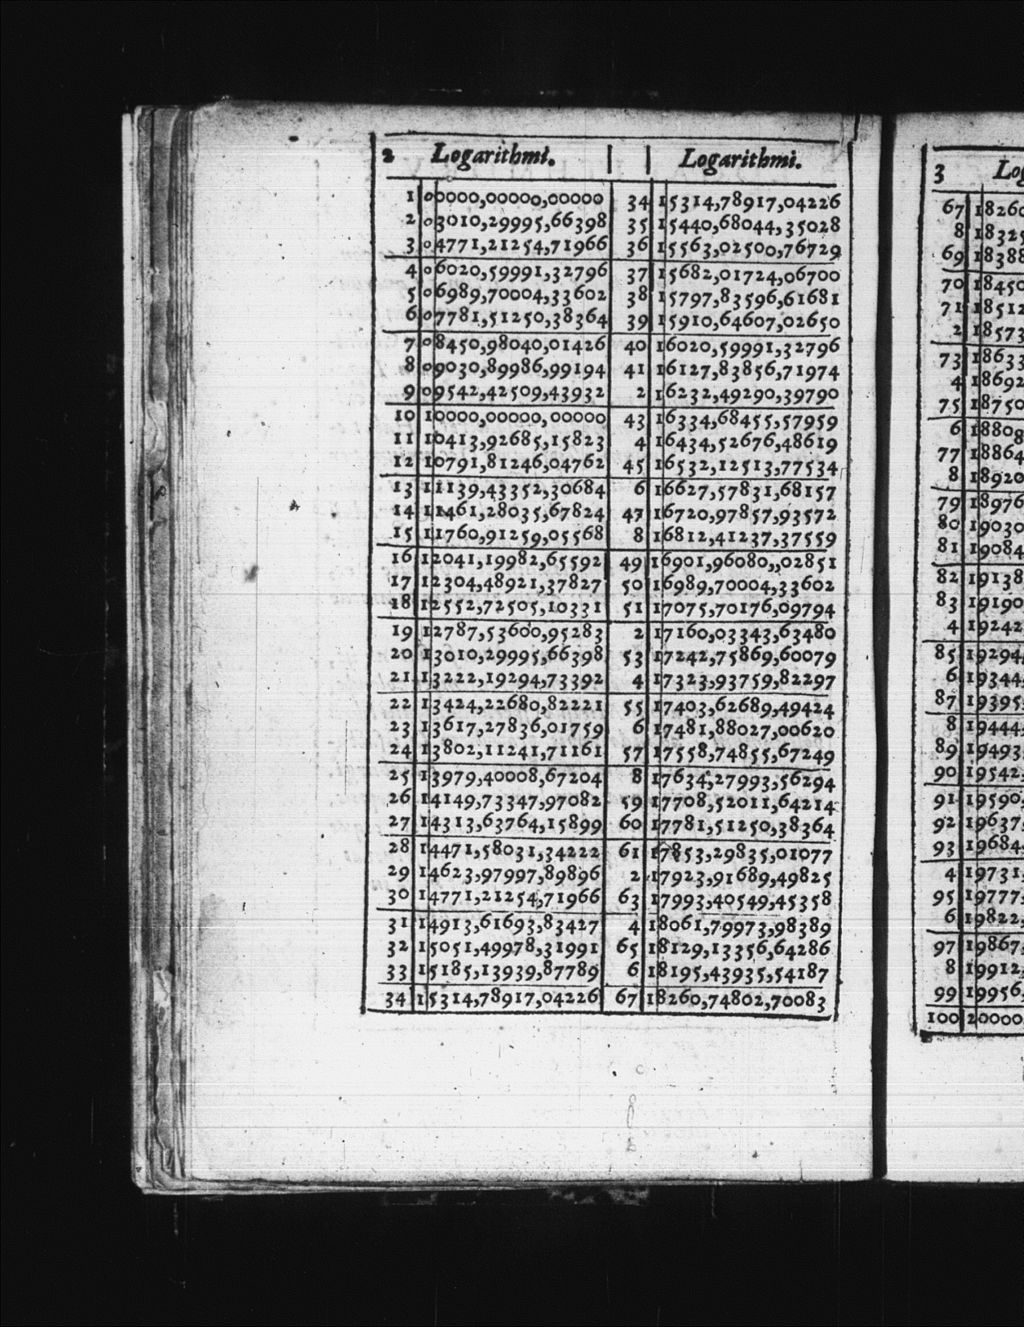
\includegraphics[height=80mm]{Logarithmorum_Chilias_Prima_page_0-67.jpg}%Figura de domínio público
\caption{Uma página do \textit{Logarithmorum Chilias Prima} de Henry Briggs, publicado em 1617, com aproximações dos logarimos em base 10 dos números inteiros de 0 à 67 com precisão de 14 casas decimais.}
\end{figure}


Vamos ilustrar como calcular $\log_2 3$ manualmente utilizando o método da bissecção. Esse método já era utilizado para calcular aproximações\footnote{Outro uso importante é para calcular raízes ou zeros de funções.} antes da invenção dos computadores, mas ainda é bastante utilizado na computação.



\begin{observation}{O método da bissecção}
Para aplicarmos o método da bissecção, tomamos uma aproximação superior e outra inferior para o número buscado, encontrando assim um intervalo no qual temos certeza em que a solução se encontra. Então tomamos o ponto médio desse intervalo como a próxima aproximação e testamos se ele é superior ou inferior ao número buscado, então basta substituirmos o respectivo extremo do intervalo por ele. Repetindo esse processo obtemos aproximações cada vez melhores para o número buscado.
\end{observation}


%Mostre aos estudantes como calcular (opcionalmente peça aos estudantes que calculem) aproximações com três casas 
%decimais de precisão, utilizando o método da bissecção ou o método de Newton (sem o uso da 
%calculadora), para $a = \sqrt{8}$, $b = \sqrt[4]{128}$ e $c=\sqrt[8]{8192}$.
%$$
%\begin{array}{|c|r|}
%\hline \sqrt{8} & \textcolor{blue}{2,828}\\
%\hline \sqrt[4]{128} & \textcolor{blue}{3,363}\\
%\hline \sqrt[8]{8192} & \textcolor{blue}{3,084}\\
%\hline
%\end{array}
%$$

\begin{ObjetivoEsp}{O método da bissecção}
{Aplicar o método da bissecção para a obtenção de aproximações sucessivas cada vez melhores.}
{1}
\end{ObjetivoEsp}

\begin{Recomenda}{O método da bissecção}
{O método é apresentado de forma repetitiva, pois essa é uma de suas característica fundamentais, e pode-se destacar que isso o torna adequado para a implementação no computador, que é uma boa ferramenta para a execução de cálculos repetitivos. A seção sobre \textit{Pensamento Computacional} explora o conceito de erro sob a ótica do computador de maneira mais explícita.

A ilustração geométrica do método esclarece o seu nome "método da bissecção", pois dividimos, vez após vez, um intervalo que contém a solução e decidimos em quais das duas metades deve estar o $\log_2 3$. }
{1}
\end{Recomenda}

O $\log_2 3$ é o expoente em que precisamos elevar $2$ para obter $3$, ou seja $2^{\log_2 3} = 3$, assim precisamos encontrar expoentes tais que 2 elevado a esses expoentes se aproxima cada vez mais de 3.  Podemos iniciar nossas tentativas com os expoentes $1$ e $2$. De fato $2^1=2<3$ e $2^2 = 4>3$, junto ao fato que as potências de 2 crescem quando crescem os expoentes, temos que $1<\log_2 3 < 2$. Para aplicar o método, escolhemos então, inicialmente, as aproximações inferior $i=1$ e superior $s=2$.

Tomamos, então a metade do intervalo $(1,2)$ como uma primeira aproximação $x=(1+2)/2 = 3/2$.
\begin{center}
\begin{tikzpicture}[scale=1.5]
\draw[black] (1,0) -- (6,0);
\draw[black] (2,-0.1) -- (2,0.1);
\draw[black] (3.5,-0.1) -- (3.5,0.1);
\draw[black] (5,-0.1) -- (5,0.1);
\node[black] at (2,-0.5) {$i=1$};
\node[black] at (5,-0.5) {$s=2$};
\node[black] at (3.5,-0.5) {$x=1{,}5$};
\draw[penvinho,->,thick] (4.5,0.5) .. controls(4.1,0.3) .. (3.9,0.05);
\node[penvinho] at (4.9,0.5) {$\log_2 3$};
\end{tikzpicture}
%\captionof{figure}{O $\log_5 100$ está no intervalo $(2,3)$.}
\end{center}

Agora precisamos verificar se $x = 3/2$ é uma aproximação superior ou inferior e fazemos isso verificando se $2^{3/2}$ é maior ou menor do que $3$, que é o mesmo que comparar $2^3=8$ com $3^2=9$, pois a raiz quadrada é uma função crescente. Como $2^3 < 3^2$, temos que $2^{3/2}<3$ e $3/2<\log_2 3$, novamente pelo fato das potências de 2 crescerem quando crescem os expoentes. Assim a nova aproximação inferior passa a ser $i=3/2$ e aproximação superior continua sendo $s=2$.

Tomamos, então a metade do intervalo $(3/2, 2)$ como uma segunda aproximação $x=(3/2+2)/2 = 7/4$. 
\begin{center}
\begin{tikzpicture}[scale=1.5]
\draw[black] (1,0) -- (6,0);
\draw[black] (2,-0.1) -- (2,0.1);
\draw[black] (3.5,-0.1) -- (3.5,0.1);
\draw[black] (5,-0.1) -- (5,0.1);
\node[black] at (2,-0.5) {$i=1{,}5$};
\node[black] at (5,-0.5) {$s=2$};
\node[black] at (3.5,-0.5) {$x=1{,}75$};
\draw[penvinho,->,thick] (4.5,0.5) .. controls(4.1,0.3) .. (3.9,0.05);
\node[penvinho] at (4.9,0.5) {$\log_2 3$};
\end{tikzpicture}
%\captionof{figure}{O $\log_5 100$ está no intervalo $(2,3)$.}
\end{center}

Agora precisamos verificar se $2^{7/4}$ é maior ou menor do que $3$, que é o mesmo que comparar $2^7=128$ com $3^4=81$, pois a raiz quarta é uma função crescente. Como $2^7 > 3^4$, temos que $2^{7/4}>\log_2 3$ e $7/4$ é uma aproximação superior. 

Tomamos, então a metade do intervalo $(3/2, 7/4)$ como uma terceira aproximação $x=(3/2+7/4)/2 = 13/8$.
\begin{center}
\begin{tikzpicture}[scale=1.5]
\draw[black] (1,0) -- (6,0);
\draw[black] (2,-0.1) -- (2,0.1);
\draw[black] (3.5,-0.1) -- (3.5,0.1);
\draw[black] (5,-0.1) -- (5,0.1);
\node[black] at (2,-0.5) {$i=1{,}5$};
\node[black] at (5,-0.5) {$s=1{,}75$};
\node[black] at (3.5,-0.5) {$x=1{,}625$};
\draw[penvinho,->,thick] (4.5,0.5) .. controls(4.1,0.3) .. (3.9,0.05);
\node[penvinho] at (4.9,0.5) {$\log_2 3$};
\end{tikzpicture}
%\captionof{figure}{O $\log_5 100$ está no intervalo $(2,3)$.}
\end{center}

Agora precisamos verificar se $2^{13/8}$ é maior ou menor do que $3$. Para fazer isso comparamos $2^{13/8}$ com $3$, que é o mesmo que comparar $2^{13}=8192$ com $3^8=6561$. Como $2^{13} > 3^8$, temos que $2^{13/8}>\log_2 3$ e $13/8$ é uma aproximação superior. 

Podemos continuar esse processo quantas vezes desejarmos, mas vamos parar com o intervalo $(3/2,13/8)$ e tomar o ponto médio dele $x=(3/2+13/8)/2=25/16$ como aproximação.
\begin{center}
\begin{tikzpicture}[scale=1.5]
\draw[black] (1,0) -- (6,0);
\draw[black] (2,-0.1) -- (2,0.1);
\draw[black] (3.5,-0.1) -- (3.5,0.1);
\draw[black] (5,-0.1) -- (5,0.1);
\node[black] at (2,-0.5) {$i=1{,}5$};
\node[black] at (5,-0.5) {$s=1{,}625$};
\node[black] at (3.5,-0.5) {$x=1{,}5625$};
\draw[penvinho,->,thick] (4.5,0.5) .. controls(4.1,0.3) .. (3.9,0.05);
\node[penvinho] at (4.9,0.5) {$\log_2 3$};
\draw [decorate,decoration={brace,amplitude=10pt},xshift=0.2,yshift=0pt]
(2,0) -- (3.5,0);
\node [black] at (2.75,0.4) {\footnotesize $0{,}0625$};
\end{tikzpicture}
\end{center}

\begin{ObjetivoEsp}{Cálculo do $\log_2 5$}
{Praticar o método da bissecção, aplicando-o no cálculo de logaritmos.}
{1}
\end{ObjetivoEsp}

\begin{Recomenda}{Cálculo do $\log_2 5$}
{O cálculo manual pode ser uma oportunidade para fixar o método da bissecção e poderia ser complementado com atividades práticas interdisciplinares de computação com a implementação do método em alguma linguagem.}
{1}
\end{Recomenda}

A aproximação para o logaritmo está boa? Pelo fato de $3/2 < \log_2 3 < 13/8$, temos certeza que $\log_2 3$ está no intervalo $(3/2,13/8)$. Contudo nossa aproximação está no centro do intervalo e à uma distância menor do que a metade do seu comprimento ($(13/8-3/2)/2= 1/16 = 0,0625$) de qualquer ponto do intervalo, inclusive $\log_2 3$. Assim garantimos que o erro em nossa aproximação é menor do que $0{,}0625$.

\begin{resposta}{Cálculo do $\log_2 5$} 
{Calcular $\log_2 5$ significa encontrar o expoente ao qual deve-se elevar $2$ para obter $5$, ou seja, é o número tal que $2^{\log_2 5} = 5$. Assim buscamos expoentes de $2$ que levem a resultados cada vez mais próximos de 5.

Como $2^2 = 4 <5<8 =2^3$, tomamos $i=2$ e $s=3$ como aproximações iniciais.

Verificamos, então, se o ponto médio $(2+3)/2=5/2$ é uma aproximação superior ou inferior. Isso é feito comparando $2^5=32$ com $5^2=25$. Como $2^5 > 5^2$ temos que $2^{5/2} > 5$ e $5/2 > \log_2 5$, pois a função exponencial $2^x$ cresce, conforme crescem os valores de $x$. Então tomamos $s=5/2=2,5$, enquanto mantemos $i=2$. A aproximação seguinte é, então, $(2+5/2)/2 = 9/4 = 2,25$.

Como $\log_2 5 \in (2, 5/2)$ e $2,25$ está a uma distância menor do que 0,25 de qualquer ponto do intervalo, temos que 2,25 é uma aproximação com o erro menor do que o pedido.}
{1}
\end{resposta}
\begin{task}{cálculo do $\log_2 5$}
Utilize o método da bissecção para calcular $\log_2 5$ com erro menor do que $0,25$. 
\end{task}

\pagebreak

\know{Logaritmos com a régua de cálculo}

\begin{ObjetivoEsp}{Logaritmos com a régua}
{\begin{itemize}
\item Observar as dificuldades inerentes à realização de operações de multiplicação com números grandes.
\item Desenvolver operações de multiplicação e divisão utilizando a soma de logaritmos.
\item Efetuar cálculos de multiplicação e divisão utilizando a régua de cálculo.
\end{itemize}}
{1}
\end{ObjetivoEsp}

\begin{Recomenda}{Logaritmos com a régua}
{A seção \textit{Para saber +: logaritmos com a régua de cálculo} é opcional. A seção realiza uma exploração das ideias que levaram ao desenvolvimento dos logaritmos, como recomenda-se às explorações históricas, que não sejam apenas fatos e anedotas desconexos das ideias e necessidades que levaram ao surgimento de determinada ideia.

Iniciamos a seção apresentado o problema da multiplicação de grandes números, que pode parecer trivial para o leitos moderno, mas que facilmente gera erros. Para ilustrar esse ponto, sugerimos na atividade \textit{Multiplicação manual} que os estudantes calculem $19683 \times 2187$ manualmente.

Nessa etapa ilustra-se como uma tabela de logaritmos pode ser utilizada para realizar multiplicações e divisões. Recomenda-se que o cálculo da atividade anterior seja realizado somando as potência de três, cujos valores poderiam estar tabelados. Para tornar esse tipo de operação mais concreta recomenda-se o desenvolvimento, das operações de multiplicação triviais listadas, com o auxílio da tabela disponível no material do aluno.

Algum estudante pode questionar que é muito mais fácil simplesmente realizar as multiplicações e divisões listadas, o que é verdade, mas cabe ressaltar que estamos realizando esses cálculos apenas para ilustrar a técnica, mas que ela é realmente útil quando trabalhamos com números grandes. Por fim, o funcionamento da régua de cálculo será baseado nesse princípio, o que é a motivação para essa discussão aqui.}
{1}
\end{Recomenda}

Antes do surgimento e popularização das calculadoras digitais, era muito laborioso efetuar todas as operações de multiplicação e divisão necessárias em muitas atividades, como no controle de estoques, na contabilidade, no cálculo de impostos e em cálculos astronômicos (principalmente ligados à navegação). Os logaritmos foram inventados para facilitar esses cálculos. Frequentemente as operações de multiplicação e divisão são consideradas triviais, 
contudo para números razoavelmente longos é fácil cometer erros nos cálculos:


\begin{resposta}{Multiplicação manual}
{Recomenda-se perguntar os resultados obtidos à turma antes de apresentar a resposta correta e espera-se obter diversos resultados distintos. \textbf{O resultado é $43046721$}, mas a experiência mostra que dificilmente algum estudante chega ao resultado correto e recomenda-se que o/a professor/a diga que tais erros eram esperados, pois é muito fácil cometer erros ao multiplicar grandes números.}
{1}
\end{resposta}
\begin{task}{Multiplicação manual}
Calcule, sem a utilização de equipamentos eletrônicos,
$$
19683 \times 2187.
$$
Verifique, com a ajuda de uma calculadora, se obteve a resposta correta.
\end{task}

Erros são bastante comuns em cálculos de multiplicação e representavam um problema sério quando os cálculos eram necessários e 
não havia nenhum 
meio eletrônico que permitisse a verificação deles. A respeito deste problema, o escocês considerado o inventor dos 
logaritmos: John Nepier \footnote{Também conhecido como John Naper ou  Ioannes Neper na versão latinizada de seu 
nome.}, 
escreveu (tradução livre) em sua obra de 1614:
\begin{quote}
Dado que nada (caros amadores apaixonados pela Matemática) é tão desagradável à prática matemática 
(freando e retardando os especialistas no cálculo) quanto as multiplicações, as divisões e as extrações de raízes 
quadradas ou cúbicas de números grandes que, além do incômodo devido ao seu tamanho, induzem a diversos erros 
perigosos; 
como consequência, eu me dediquei a procurar por que meios seguros e cômodos poderia me livrar destas 
dificuldades.

\raggedleft \textit{John Napier - Mirifici logarithmorum canonis descriptio} 
\end{quote}

O cálculo realizado acima pode ser feito de modo muito mais rápido se tivermos uma tabela com os valores das potências de $3$ e levarmos em conta que:
\begin{itemize}
 \item $3^5=2187$,
  \item $3^7=19683$,
   \item $19683 \times 2187 = 3^5 \times 3^7 = 3^{12} = 43046721$.
\end{itemize}


Assim, podemos utilizar a Tabela \ref{potencias2_log} para fazer cálculos de multiplicação ou divisão, somando ou subtraindo  os logaritmos e localizando o resultado correspondente a soma, ao invés de multiplicar explicitamente:
\begin{itemize}
 \item $5 \times 4 \approx 2^{2{,}32} \times 2^2 = 2^{2{,}32 + 2} = 2^{4{,}32} \approx 20$;
 \item $3 \times 5 \approx 2^{1{,}58} \times 2^{2{,}32} = 2^{1{,}58 + 2{,}32} = 2^{3{,}9} \approx 15$;
 \item $3 \times 9 \approx 2^{1{,}58} \times 2^{3{,}16} = 2^{1{,}58+3{,}16} = 2^{4{,}74} \approx 27$.
  \item $20 \div 4 \approx 2^{4{,}32} \div 2^{2} = 2^{4,32-2} = 2^{2{,}32} \approx 5$.
 \end{itemize}

\begin{ObjetivoEsp}{Multiplicações com uma tabela}
{Entender como uma tabela de logaritmos pode ser utilizada para efetuar cálculos de multiplicação.}
{1}
\end{ObjetivoEsp}

\begin{Recomenda}{Multiplicações com uma tabela}
{Nessa etapa busca-se ilustrar como a multiplicação de dois números pode ser realizada utilizando uma tabela. Isso é efetuado somando os logaritmos dos números e encontrando o valor dessa soma na tabela. Os cálculos efetuados são simples devido as limitações de nossa tabela e buscam apenas mostrar o princípio, que será fundamental para os cálculos com a régua de cálculo.

Essa explicação pode ser transformada em uma atividade se o/a professor/a achar necessário.}
{1}
\end{Recomenda}

Apesar dos cálculos da soma dos expoentes não darem, necessariamente, os valores exatos que temos na 
tabela, buscamos o que melhor se aproxima. Fazemos isso pois sabemos que o produto de dois naturais é novamente um 
natural e temos todos os naturais até 30 listados na tabela.


Napier escreveu um livro inteiro de logaritmos tabelados para consulta e utilização em cálculos. Henri Briggs, um dos pais dos logaritmos, publicou um livro\footnote{Há uma foto de uma página do livro no \textit{Para saber +: sem ferramentas de cálculo...}} com todos os logaritmos em base 10 dos números naturais de $1$ à $20000$. Mas, não é muito prático carregarmos uma longa tabela por aí. Para lidar com esse problema, William Oughtred  (1574 – 1660) inventou réguas de cálculo.
\begin{figure}
\caption{Uma régua de cálculo}
\centering
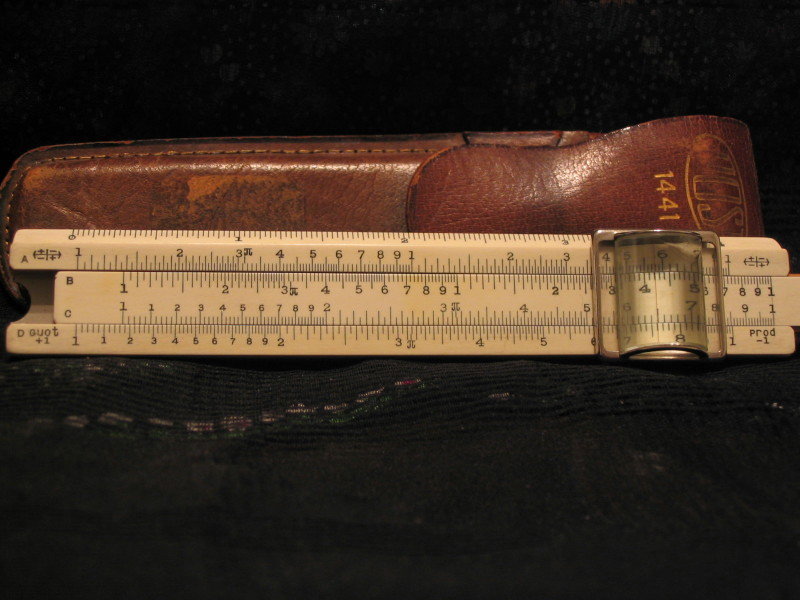
\includegraphics[width=0.5\linewidth]{Figuras/Reguadecalculo}\\
{\textbf{Fonte:} Slide Rule em Flickr / Usuário: The Last Cookie}% https://www.flickr.com/photos/cabeel/2197888941/in/photostream/
\end{figure}
A régua linear de Oughtred efetuava multiplicações e divisões com duas escalas logarítmicas, fazendo as partes da régua deslizarem uma sobre a outra. A régua de cálculo, com suas variantes, foi, durante mais de 300  anos, uma ferramenta indispensável para engenheiros e cientistas, era um presente dado de pais para filhos ao final do 
ginásio. Ela aprimorada por diversos cientistas e engenheiros até chegar em sua versão atual. Estudaremos uma régua de cálculo simplificada nas atividades seguintes.


\textbf{A Régua de Cálculo}

Na régua aritmética ou linear, o comprimento 1cm corresponde ao número 1, o comprimento 2 cm corresponde ao número 2 e assim sucessivamente. Na régua de cálculo logarítmica de base 2, o número 1 corresponde ao comprimento do logaritmo de 1 em base 2, o número 2 corresponde ao comprimento do logaritmo de 2 e assim por diante. A Figura \ref{Reguas} 
ilustra uma régua de cálculo formada por duas partes, cada uma com uma linha central e uma escala linear, ambas na cor 
cinza, e uma escala logarítmica na cor preta. Note que na escala logarítmica marcamos, por exemplo, o número 3 à distância 1,59 do 
ponto inicial da escala, o número 1, pois $\log_2 3 \approx 1{,}59$.

\begin{center}
\captionof{figure}{Uma régua de cálculo e sua utilização calculando 4x2 e 4x3.}\label{Reguas}
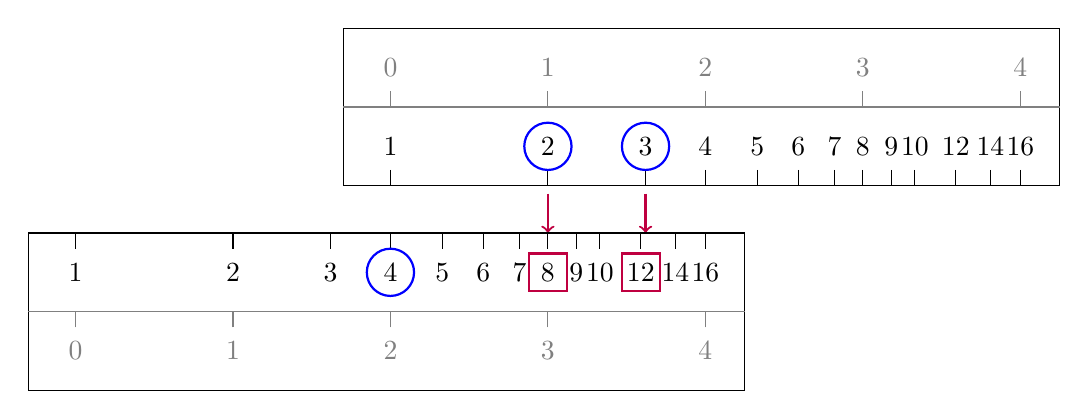
\begin{tikzpicture}[scale=2]
 \fill [white] (1.7,1.3) rectangle (6.25,2.3);
\draw (1.7,1.3)--(6.25,1.3);
 \draw (1.7,2.3)--(6.25,2.3);
 \draw (1.7,1.3)--(1.7,2.3);
 \draw (6.25,1.3)--(6.25,2.3);
 \draw (2,1.4)--(2,1.3);
 \node at (2,1.55) {1};
  \draw (3,1.4)--(3,1.3);
 \node at (3,1.55) {2};
 \draw[blue,thick] (3,1.55) circle (0.15cm);
  \draw[purple,thick,->] (3,1.25) -- (3,1);
   \draw (3.62,1.4)--(3.62,1.3);
 \node at (3.62,1.55) {3};
 \draw[blue,thick] (3.62,1.55) circle (0.15cm);
   \draw[purple,thick,->] (3.62,1.25) -- (3.62,1);
   \draw (4,1.4)--(4,1.3);
 \node at (4,1.55) {4};
   \draw (4.33,1.4)--(4.33,1.3);
 \node at (4.33,1.55) {5};
   \draw (4.59,1.4)--(4.59,1.3);
 \node at (4.59,1.55) {6};
   \draw (4.82,1.4)--(4.82,1.3);
 \node at (4.82,1.55) {7};
   \draw (5,1.4)--(5,1.3);
 \node at (5,1.55) {8};
   \draw (5.18,1.4)--(5.18,1.3);
 \node at (5.18,1.55) {9};
   \draw (5.33,1.4)--(5.33,1.3);
 \node at (5.33,1.55) {10};
    \draw (5.59,1.4)--(5.59,1.3);
 \node at (5.59,1.55) {12};
    \draw (5.81,1.4)--(5.81,1.3);
 \node at (5.81,1.55) {14};
    \draw (6,1.4)--(6,1.3);
 \node at (6,1.55) {16};
   \draw[gray] (1.7,1.8)--(6.25,1.8);
   \draw[gray] (2,1.9)--(2,1.8);
 \node[gray] at (2,2.05) {0};
    \draw[gray] (3,1.9)--(3,1.8);
 \node[gray] at (3,2.05) {1};
    \draw[gray] (4,1.9)--(4,1.8);
 \node[gray] at (4,2.05) {2};
    \draw[gray] (5,1.9)--(5,1.8);
 \node[gray] at (5,2.05) {3};
    \draw[gray] (6,1.9)--(6,1.8);
 \node[gray] at (6,2.05) {4};
  \fill [white] (-0.3,0) rectangle (4.25,1);
 \draw (-0.3,0)--(4.25,0);
 \draw (-0.3,1)--(4.25,1);
 \draw (-0.3,0)--(-0.3,1);
 \draw (4.25,0)--(4.25,1);
 \draw (0,0.9)--(0,1);
 \node at (0,0.75) {1};
  \draw (1,0.9)--(1,1);
 \node at (1,0.75) {2};
   \draw (1.62,0.9)--(1.62,1);
 \node at (1.62,0.75) {3};
   \draw (2,0.9)--(2,1);
 \node at (2,0.75) {4};
\draw[blue,thick] (2,0.75) circle (0.15cm);
 \draw (2.33,0.9)--(2.33,1);
 \node at (2.33,0.75) {5};
   \draw (2.59,0.9)--(2.59,1);
 \node at (2.59,0.75) {6};
   \draw (2.82,0.9)--(2.82,1);
 \node at (2.82,0.75) {7};
   \draw (3,0.9)--(3,1);
 \node at (3,0.75) {8};
     \draw[purple,thick] (2.88,0.63) rectangle (3.12,0.87);
   \draw (3.18,0.9)--(3.18,1);
 \node at (3.18,0.75) {9};
   \draw (3.33,0.9)--(3.33,1);
 \node at (3.33,0.75) {10};
    \draw (3.59,0.9)--(3.59,1);
 \node at (3.59,0.75) {12};
      \draw[purple,thick] (3.47,0.63) rectangle (3.71,0.87);
    \draw (3.81,0.9)--(3.81,1);
 \node at (3.81,0.75) {14};
    \draw (4,0.9)--(4,1);
 \node at (4,0.75) {16};
  \draw[gray] (-0.3,0.5)--(4.25,0.5);
   \draw[gray] (0,0.4)--(0,0.5);
 \node[gray] at (0,0.25) {0};
    \draw[gray] (1,0.4)--(1,0.5);
 \node[gray] at (1,0.25) {1};
    \draw[gray] (2,0.4)--(2,0.5);
 \node[gray] at (2,0.25) {2};
    \draw[gray] (3,0.4)--(3,0.5);
 \node[gray] at (3,0.25) {3};
    \draw[gray] (4,0.4)--(4,0.5);
 \node[gray] at (4,0.25) {4};
 \end{tikzpicture}\\
\vspace{3mm}
\textbf{Fonte:} Logaritmos e a régua de cálculo, Pedrosa \& Adames.
\end{center}
\begin{ObjetivoEsp}{Régua em base 2}
{Entender o mecanismo de funcionamento da régua de cálculo.}
{1}
\end{ObjetivoEsp}

\begin{Recomenda}{Régua em base 2}
{Nessa etapa busca-se ilustrar como a régua de cálculo funciona em uma régua de cálculo de base $2$, que pode ser mais natural para os estudantes. Recomenda-se que o professor mostre como fazer cálculos com a régua dessa base e, se possível, construa o par de réguas de base $2$ em maior tamanho para mostrar aos estudantes o funcionamento.

Recomenda-se que seja destacado que, ao colocarmos as réguas lado a lado, estamos somando os logaritmos dos números na escala linear e, de acordo com os exemplos anteriores, obtemos o resultado correto na multiplicação.}
{1}
\end{Recomenda}

Podemos utilizar as réguas de cálculo para fazer multiplicações ou divisões.

Para multiplicar $a \times b$, basta colocar as duas metades da régua uma sobre a outra, como na figura, colocando o número 1 da metade 
superior da régua sobre $a$. O resultado estará então abaixo de $b$. Como ilustra a Figura \ref{Reguas} nas 
multiplicações 4x2 e 4x3.

\begin{center}
\captionof{figure}{Uma régua de cálculo utilizada para calcular $14 \div 7$.}\label{Reguas}
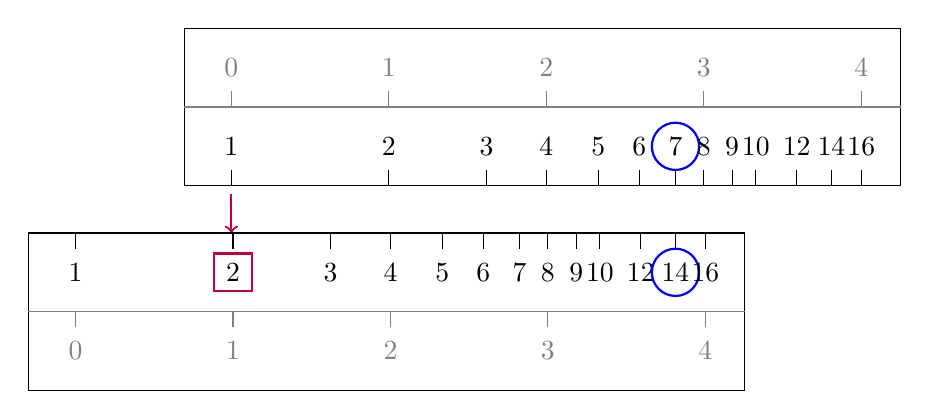
\begin{tikzpicture}[scale=2]
 \fill [white] (0.69,1.3) rectangle (5.24,2.3);
\draw (0.69,1.3)--(5.24,1.3);
 \draw (0.69,2.3)--(5.24,2.3);
 \draw (0.69,1.3)--(0.69,2.3);
 \draw (5.24,1.3)--(5.24,2.3);
 \draw (0.99,1.4)--(0.99,1.3);
 \node at (0.99,1.55) {1};
  \draw (1.99,1.4)--(1.99,1.3);
 \node at (1.99,1.55) {2};
   \draw (2.61,1.4)--(2.61,1.3);
 \node at (2.61,1.55) {3};
   \draw[purple,thick,->] (0.99,1.25) -- (0.99,1);
   \draw (2.99,1.4)--(2.99,1.3);
 \node at (2.99,1.55) {4};
   \draw (3.32,1.4)--(3.32,1.3);
 \node at (3.32,1.55) {5};
   \draw (3.58,1.4)--(3.58,1.3);
 \node at (3.58,1.55) {6};
   \draw (3.81,1.4)--(3.81,1.3);
 \node at (3.81,1.55) {7};
  \draw[blue,thick] (3.81,1.55) circle (0.15cm);
   \draw (3.99,1.4)--(3.99,1.3);
 \node at (3.99,1.55) {8};
   \draw (4.17,1.4)--(4.17,1.3);
 \node at (4.17,1.55) {9};
   \draw (4.32,1.4)--(4.32,1.3);
 \node at (4.32,1.55) {10};
    \draw (4.58,1.4)--(4.58,1.3);
 \node at (4.58,1.55) {12};
    \draw (4.8,1.4)--(4.8,1.3);
 \node at (4.8,1.55) {14};
    \draw (4.99,1.4)--(4.99,1.3);
 \node at (4.99,1.55) {16};
   \draw[gray] (0.69,1.8)--(5.24,1.8);
   \draw[gray] (0.99,1.9)--(0.99,1.8);
 \node[gray] at (0.99,2.05) {0};
    \draw[gray] (1.99,1.9)--(1.99,1.8);
 \node[gray] at (1.99,2.05) {1};
    \draw[gray] (2.99,1.9)--(2.99,1.8);
 \node[gray] at (2.99,2.05) {2};
    \draw[gray] (3.99,1.9)--(3.99,1.8);
 \node[gray] at (3.99,2.05) {3};
    \draw[gray] (4.99,1.9)--(4.99,1.8);
 \node[gray] at (4.99,2.05) {4};
  \fill [white] (-0.3,0) rectangle (4.25,1);
 \draw (-0.3,0)--(4.25,0);
 \draw (-0.3,1)--(4.25,1);
 \draw (-0.3,0)--(-0.3,1);
 \draw (4.25,0)--(4.25,1);
 \draw (0,0.9)--(0,1);
 \node at (0,0.75) {1};
  \draw (1,0.9)--(1,1);
 \node at (1,0.75) {2};
 \draw[purple,thick] (0.88,0.63) rectangle (1.12,0.87);
   \draw (1.62,0.9)--(1.62,1);
 \node at (1.62,0.75) {3};
   \draw (2,0.9)--(2,1);
 \node at (2,0.75) {4};
 \draw (2.33,0.9)--(2.33,1);
 \node at (2.33,0.75) {5};
   \draw (2.59,0.9)--(2.59,1);
 \node at (2.59,0.75) {6};
   \draw (2.82,0.9)--(2.82,1);
 \node at (2.82,0.75) {7};
   \draw (3,0.9)--(3,1);
 \node at (3,0.75) {8};
   \draw (3.18,0.9)--(3.18,1);
 \node at (3.18,0.75) {9};
   \draw (3.33,0.9)--(3.33,1);
 \node at (3.33,0.75) {10};
    \draw (3.59,0.9)--(3.59,1);
 \node at (3.59,0.75) {12};
    \draw (3.81,0.9)--(3.81,1);
 \node at (3.81,0.75) {14};
  \draw[blue,thick] (3.81,0.75) circle (0.15cm);
    \draw (4,0.9)--(4,1);
 \node at (4,0.75) {16};
  \draw[gray] (-0.3,0.5)--(4.25,0.5);
   \draw[gray] (0,0.4)--(0,0.5);
 \node[gray] at (0,0.25) {0};
    \draw[gray] (1,0.4)--(1,0.5);
 \node[gray] at (1,0.25) {1};
    \draw[gray] (2,0.4)--(2,0.5);
 \node[gray] at (2,0.25) {2};
    \draw[gray] (3,0.4)--(3,0.5);
 \node[gray] at (3,0.25) {3};
    \draw[gray] (4,0.4)--(4,0.5);
 \node[gray] at (4,0.25) {4};
 \end{tikzpicture}\\
\end{center}

Para dividir $a / b$, basta colocar as duas metades da régua uma sobre a outra, como na figura, colocando o número $b$ da metade 
superior da régua sobre $a$. O resultado estará então abaixo do número $1$. Como pode ser visto no resultado de $14 \div 7$, que está abaixo do número $1$.

Isso funciona pois ao colocarmos as réguas assim, estamos adicionando ou  subtraindo os comprimentos dos logaritmos dos respectivos números (na escala linear em cinza claro).

Por fim ainda temos o problema que a base dois cresce muito rapidamente. Para resolver isso podemos tomar uma que seja bem próxima de 1 e um pouco maior.

Produzimos réguas de cálculo, que estão no final do capítulo, utilizando a base $x = 10^{1/50}\approx 1{,}04713$, de modo que $\log_{x}100=100$. As graduações na régua correspondem aos logaritmos em base $x$ dos números de 0 a 10 com uma casa decimal de precisão e dos números naturais de 11 até 100. A régua também contém uma escala linear e as posições dos números na escala logarítmica correspondem aos valores dos logaritmos daqueles números na base $x$. A Figura \ref{ReguaCalculo} ilustra a régua.


\captionof{figure}{A régua de cálculo que acompanha este material.}\label{ReguaCalculo}
\begin{figure}[!ht]
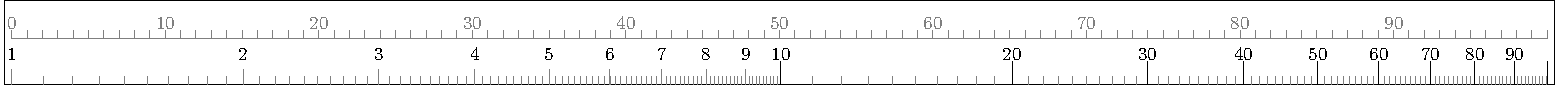
\includegraphics[width=\linewidth]{Figuras/Ruler1.pdf}
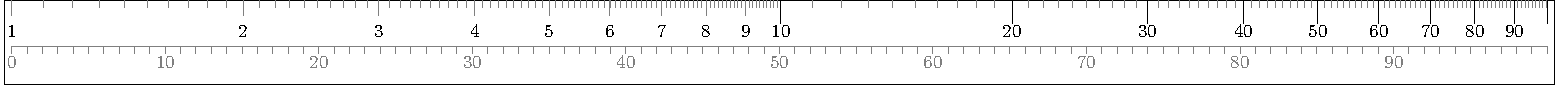
\includegraphics[width=\linewidth]{Figuras/Ruler2.pdf}
\end{figure}
\vspace{3mm}
\begin{center}
\textbf{Fonte:} Logaritmos e a régua de cálculo, Pedrosa \& Adames.
\end{center}

\begin{ObjetivoEsp}{Cálculos com a régua}
{Aplicar uma régua de cálculo em operações de multiplicação e divisão.}
{1}
\end{ObjetivoEsp}

\begin{Recomenda}{Cálculos com a régua}
{Recomenda-se que se destaque um problema na utilização da régua em base dois: os números crescem rápido demais. Aqui seria possível questionar aos alunos como esse problema poderia ser resolvido, antes de apresentar a resposta: tomar uma base menor (mas que ainda precisará ser maior do que $1$, caso contrário teríamos uma escala decrescente na régua).

Recomenda-se então que os estudantes utilizem, em grupos, as réguas disponíveis com o material para efetuar as operações indicadas. O/A professor/a pode tirar cópias das réguas no anexo, recortá-las e entregar aos alunos para que não sejam removidas do material.}
{1}
\end{Recomenda}

\begin{task}{Cálculos com a régua}

Em pequenos grupos, vamos utilizar as réguas de cálculo para efetuar os seguintes cálculos:
\begin{enumerate}
 \item 9 x 7. %\textcolor{blue}{Basta colocar deslizar a metade superior de modo que o número 1 esteja sobre o número 9 da régua inferior e observar a resposta 63 abaixo do número 7 da metade superior.}
 \item 3,5 x 4.% \textcolor{blue}{Basta colocar deslizar a metade superior de modo que o número 1 esteja sobre o número 3,5 da régua inferior e observar a resposta 14 abaixo do número 4 da metade superior.}
 \item 2,8 x 2,5.% \textcolor{blue}{Basta colocar deslizar a metade superior de modo que o número 1 esteja sobre o número 2,8 da régua inferior e observar a resposta 7 abaixo do número 2,5 da metade superior.}
 \item 28 x 25.% \textcolor{blue}{Apesar dos números 28 e 25 estarem nas duas metades da régua, a posição onde estaria a reposta fica além do comprimento da régua, mas podemos realizar esse cálculo lembrando que $28 \times 25 = 2,8 \times 2,5 \times 10^2 = 7 \times 10^2 = 700$.}
 \item 3,2 x 3,1.% \textcolor{blue}{Ao aplicarmos o procedimento a resposta parece dar $9,9$. Isso ocorre pois há um limite para a escala de graduações escrita na régua, que tem precisão máxima de uma casa decimal para números menores do que 10 e precisão apenas da parte inteira para números maiores do que 10. A resposta exata seria 9,92 e a resposta 9,9 é uma aproximação para ela.}
\item 5,8 x 9,3.% \textcolor{blue}{A régua mostra a aproximação 54, que está bastante próxima da resposta exata 53,94.}
\item 583 x 93.% \textcolor{blue}{$583 \times 93 = 5,83 \times 9,3 \times 10^3 \approx 54 \times 10^3 = 54000$, que é uma aproximação para a resposta exata 54219.}
\item 78326 x 648.% \textcolor{blue}{$78326 \times 648 = 7,8326 \times 6,48 \times 10^6 \approx 51 \times 10^6 = 51000000$, que é uma aproximação para a resposta exata 50755248.}
\item 56 $\div$ 7.% \textcolor{blue}{Basta colocar deslizar a metade superior de modo que o número 7 esteja sobre o número 56 da régua inferior e observar a resposta 8 abaixo do número 1 da metade superior. Essa operação funciona pois a resposta para $56 \div 7$ é o número que multiplicado por 7 da 56, de modo que, ao colocarmos o número 7 sobre o número 56, o número abaixo do 1 é a resposta para $56 \div 7$.}
\item 58 $\div$ 4. %\textcolor{blue}{A régua mostra um valor entre 14 e 15, nesses casos podemos tomar a média entre eles, 14,5, que, por acaso, acaba coincidindo com a resposta exata.}
\item 93 $\div$ 5.% \textcolor{blue}{A régua mostra um valor entre 18 e 19, nesses casos podemos tomar a média entre eles, 18,5, que aproxima resposta exata 18,6.}
\item 476 $\div$ 93.% \textcolor{blue}{$476 \div 93 = 47,6 \div 9,3 \approx 5,1$, que é uma aproximação para a resposta dada pela calculadora 5,11827957 (que é apenas uma aproximação...).}
\item 7345 $\div$ 57.% \textcolor{blue}{$7345 \div 57 =73,45 \div 5,7 \times 10\approx 12,5 \times 10 = 125$, que é uma aproximação para a resposta dada pela calculadora 128,859649123 (que é apenas uma aproximação...).}
\end{enumerate}
\end{task}
\begin{resposta}{Cálculos com a régua}
{\begin{enumerate}[label=\alph*)]
\item[] Nessas atividades basta deslizar a metade superior de modo que o número 1 esteja sobre o primeiro dos fatores e observar a resposta abaixo do segundo fator na régua superior.
\item $9 \times 7 = 63$.
 \item $3{,}5 \times 4 = 14$.
 \item $2{,}8 \times 2,5 = 7$.
 \item $28 \times 25 = 700$. Apesar dos números $28$ e $25$ estarem nas duas metades da régua, a posição onde estaria a reposta fica além do comprimento da régua, mas podemos realizar esse cálculo lembrando que $28 \times 25 = 2{,}8 \times 2{,}5 \times 10^2 = 7 \times 10^2 = 700$.
 \item $3{,}2 \times 3{,}1 \approx 9{,}9$. Ao aplicarmos o procedimento a resposta parece dar $9,9$. Isso ocorre pois há um limite para a escala de graduações escrita na régua, que tem precisão máxima de uma casa decimal para números menores do que $10$ e precisão apenas da parte inteira para números maiores do que $10$. A resposta exata seria $9{,}92$ e a resposta $9{,}9$ é uma aproximação para ela.
\item $5{,}8 \times 9{,}3 \approx 54$. A régua mostra a aproximação $54$, que está bastante próxima da resposta exata $53{,}94$.
\item $583 \times 93\approx 54000$. $583 \times 93 = 5,83 \times 9,3 \times 10^3 \approx 54 \times 10^3 = 54000$, que é uma aproximação para a resposta exata $54219$.
\item $78326 \times 648 \approx 51000000$. $78326 \times 648 = 7,8326 \times 6,48 \times 10^6 \approx 51 \times 10^6 = 51000000$, que é uma aproximação para a resposta exata $50755248$.
\item $56 \div 7 = 8$.
\item $58 \div 4 = 14{,}5$. A régua mostra um valor entre $14$ e $15$, nesses casos podemos tomar a média entre eles, $14{,}5$, que, por acaso, acaba coincidindo com a resposta exata.
\item $93 \div 5 \approx 18{,}6$. A régua mostra um valor entre $18$ e $19$, nesses casos podemos tomar a média entre eles, $18{,}5$, que aproxima resposta exata $18{,}6$.
\item $476 \div 93 \approx 5{,}1$. $476 \div 93 = 47{,}6 \div 9{,}3 \approx 5{,}1$, que é uma aproximação para a resposta dada pela calculadora $5{,}11827957$ (que é apenas uma aproximação...).
\item $7345 \div 57 \approx 125$. $7345 \div 57 =73,45 \div 5{,}7 \times 10\approx 12{,}5 \times 10 = 125$, que é uma aproximação para a resposta dada pela calculadora $128{,}859649123$ (que é apenas uma aproximação...).
\end{enumerate}}
{1}
\end{resposta}

\pagebreak

\know{Ajustes de curvas}

\begin{ObjetivoEsp}{Ajustes de curvas}
{Utilizar ferramentas computacionais na busca de funções que melhor aproximem dados reais.}
{1}
\end{ObjetivoEsp}

\begin{Recomenda}{Ajustes de curvas}
{O desenvolvimento dessa seção é opcional e pretende explorar a aproximação de dados reais através de funções conhecidas. A atividade propõe analisar a adequação do ajuste de curvas aos dados reais utilizando ferramentas matemáticas e computacionais (já desenvolvidas no applet do GeoGebra relacionado), relacionando-se à habilidade EM13MAT104.

Se o/a professor/a achar adequado no contexto da turma e tiver disponibilidade de tempo, seria possível estender a atividade para as outras medidas listadas (colocando os dados no \textit{applet} fazendo discussões similares).}
{1}
\end{Recomenda}

Quando buscamos uma função para aproximar dados reais, podemos escolher que tipo de função parece mais adequada (o que pode ser um pouco subjetivo). Contudo, quando escolhemos um tipo de função, que valores escolhemos para os coeficientes dessa função? Por exemplo, se os dados parecem crescer como uma função logarítmica, qual deve ser a base? Para determinarmos essas constantes existem métodos mas que muitos programas de computador podem calcular automaticamente.

A caderneta de saúde abaixo traz as medidas (nas datas especificadas) da idade, do peso, da altura e do perímetro encefálico de uma criança.
\begin{center}
\captionof{figure}{Dados médicos na carteirinha de uma criança.}
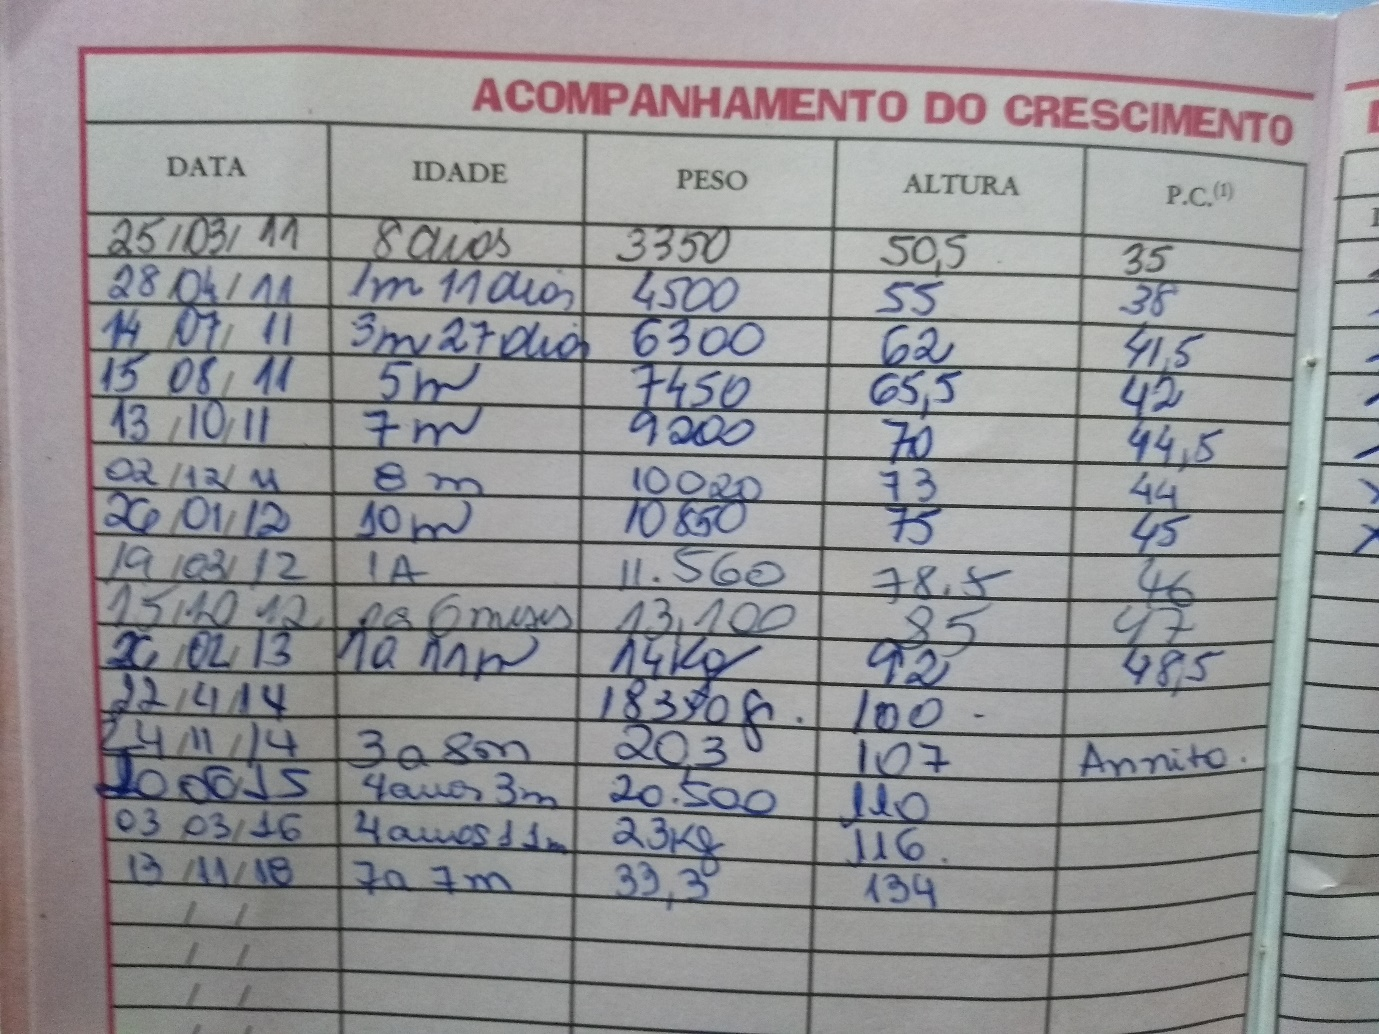
\includegraphics[width=0.8\linewidth]{Figuras/Caderneta.png}
\end{center}

Anotamos os dados de idade e altura no GeoGebra, no endereço abaixo, e utilizamos as funções do programa para aproximar os dados utilizando curvas do tipo: exponencial, logarítmica, linear, logística, potência e polinomial.

https://www.geogebra.org/calculator/za7dq64a \begin{minipage}{0.3\linewidth}
\includegraphics[width=\linewidth]{Figuras/QRcode_ajuste_curvas.png}\end{minipage}

\begin{ObjetivoEsp}{Para refletir}
{\begin{itemize}
\item Analisar a utilização de diversas funções no ajuste de curvas de dados reais.
\item Interpretar criticamente o ajuste de curvas utilizando funções conhecidas, contextualizando a situação na realidade.
\end{itemize}}
{1}
\end{ObjetivoEsp}

\begin{Recomenda}{Para refletir}
{Recomenda-se a observação das funções ajustadas no applet do GeoGebra, seguida da reflexão sobre a adequação das funções escolhidas, que pode levar em conta fatores conhecidos, como o fato que crianças crescem mais rápido do que adultos e que seres humanos atingem suas alturas máximas no início da vida adulta. Também pode ser importante discutir as limitações dos modelos, que não se aplicariam à velhice, quando nossa altura começa a diminuir.}
{1}
\end{Recomenda}

\begin{reflection}
Vamos observar as funções mostradas pelo \textit{applet}. Quais dos ajustes parecem adequados ao crescimento da altura de uma pessoa? Quais levariam a previsões absurdas? Justifique os motivos que o levaram a realizar essas escolhas.
\end{reflection}

\begin{resposta}{Para refletir}
{Observa-se que as funções exponencial, linear e polinomial tem crescimento muito rápido para valores maiores que os dados apresentados. Isso levaria a previsões de crescimento que não condizem com seres humanos. As funções logarítmica e logística crescem muito lentamente para valores maiores do que aqueles dos dado apresentados, gerando valores abaixo dos esperados para a altura de um ser humano saudável. Por eliminação das outras possibilidades, a função potência parece ser mais adequada à situação.}
{1}
\end{resposta}

Foge dos objetivos desse material estudar em detalhes os métodos para encontrar as funções que \textit{melhor aproximam} os dados reais de cada um dos tipos. Contudo um dos métodos, chamado de \textit{regressão linear} está relacionado com os logaritmos.

\begin{knowledge}
A \textit{regressão linear} é um método utilizado com frequência para encontrar a função exponencial $y(x) =a \times b^x$ que melhor aproxima dados reais e consiste em aplicar logaritmos dos dois lados da equação, obtendo $\log y = \log a + x \log b$, que é uma equação linear do tipo $v = c + dx$, com $v = \log y$ e constantes $c=\log a$ e $d=\log b$. Essa nova equação pode ser ajustada aos logaritmos dos dados reais por um método chamado de mínimos quadrados, encontrando os melhores valores para $c$ e $d$ e, então, achamos $a= 10^c$ e $b=10^d$.
\end{knowledge}


\begin{ObjetivoEsp}{Regressão linear}
{\begin{itemize}
\item Analisar uma situação real a partir de dados concretos, com auxilio da tecnologia, e fazer previsões sobre valores futuros.
\item Avaliar criticamente os resultados obtidos.
\end{itemize}}
{1}
\end{ObjetivoEsp}

\begin{task}{Regressão linear}
Utilizando os dados reais do número de casos nos Estados Unidos (fonte: Our World in Data) entre 22/01/2020 e 21/03/2020, aplicamos regressão linear com uma ferramenta computacional para estimar o número de casos pela fórmula $f(t) = 0{,}000275279 \times 1{,}36451^t$, onde $t=0$ representa o dia 22/01 e $t= 59$ o dia 21/03. %(Ref: https://towardsdatascience.com/modeling-exponential-growth-49a2b6f22e1f)

Utilizando a fórmula, quantos dias seriam necessários para que a pandemia ultrapassasse 100.000 infectados naquele país?
\end{task}

Vamos comparar os dados obtidos pela fórmula com os dados reais.
\begin{center}
\captionof{table}{Total de Casos nos E.U.A.}
\begin{tabular}{|c|c|c|c|c|c|c|}
\hline
& \cellcolor[HTML]{00A59D} 22/03 & \cellcolor[HTML]{00A59D}  23/03 & \cellcolor[HTML]{00A59D} 24/03 & \cellcolor[HTML]{00A59D}  25/03 &
\cellcolor[HTML]{00A59D} 26/03 & \cellcolor[HTML]{00A59D}  27/03\\
\hline Dados reais & 33.404 & 44.183 & 54.453 & 68.440 & 85.356 & 103.321\\
\hline Previsão da função & 34.544 & 47.136 & 64.317 & 87.762 & 119.752 & 163.403\\
\hline
\end{tabular}
\end{center}
Os valores são próximos no começo, mas começam a ficar distintos. Explicamos isso pelo fato da pandemia não se desenvolver livremente, mas há reações da população e das autoridades, como medidas sanitárias, que podem reduzir as taxas de infecção.


\begin{resposta}{Regressão linear}
{\begin{align*}
&100000 \approx 0{,}000275 \times 1{,}36451^t,\\
\Rightarrow& 1{,}36451^t \approx 363267811{,}92,\\
\Rightarrow& t \approx \log_{1{,}36451} 363267811{,}9 \approx 63{,}42
\end{align*}
Assim a fórmula estaria prevendo que o primeiro dia com mais de 100.000 casos seria o 64$^o$ dia de pandemia, o dia 26/03/2020.}
{1}
\end{resposta}

\pagebreak

\know{Logaritmos e progressões}

\begin{ObjetivoEsp}{Logaritmos e progressões}
{\begin{itemize}
\item Conhecer o desenvolvimento histórico das ideias envolvendo logaritmos.
\item Entender a relação dos logaritmos aos conteúdos de P.A. e P.G.
\end{itemize}}
{1}
\end{ObjetivoEsp}

\begin{Recomenda}{Logaritmos e progressões}
{Essa atividade é opcional, caso haja espaço no cronograma e o desejo de explorar o desenvolvimento de ideias da história da matemática. Quando Napier desenvolveu seus logaritmos, eram frequentes as construções matemáticas envolvendo movimentos e Napier explicou suas ideias sobre logaritmos nesses termos.

No movimento proposto por Napier, as posições de dois objetos eram observadas a intervalos regulares de tempo. Como o primeiro objeto move-se a velocidade constante, suas posições formam uma P.A. Já o segundo move-se uma quantidade de unidades proporcional à sua distância da origem, formando uma P.G. A atividade propõem que isso seja verificado em um exemplo concreto.

Após a atividade, recomenda-se que se reforce a interpretação de que o logaritmo de um termo da P.G é o respectivo termo da P.A.

Por fim essa relação entre logaritmos e as progressões pode ser associada à habilidade da BNCC - EM13MAT508: Identificar e associar progressões geométricas (PG) a funções exponenciais de domínios discretos, para análise de propriedades, dedução de algumas fórmulas e resolução de problemas.}
{1}
\end{Recomenda}


Napier pensava nos logaritmos como produzidos por um movimento dinâmico. Traduzimos isso pensando em dois objetos $P$ e $Q$ movendo-se sobre duas semi-retas, um partindo da origem 0 e o outro do número 1, de modo que o  primeiro desloca-se com velocidade constante, mas o segundo tem velocidade proporcional a distância que ele está da origem da semi-reta. Assim, se tomarmos intervalos de tempo igualmente espaçados $T, 2T, 3T, 4T, \ldots$, obtemos posições distintas $P_1,P_2, \ldots$ e $Q_1,Q_2, \ldots$ para os dois objetos, como ilustra a Figura \ref{Movimento}.  

\begin{center}
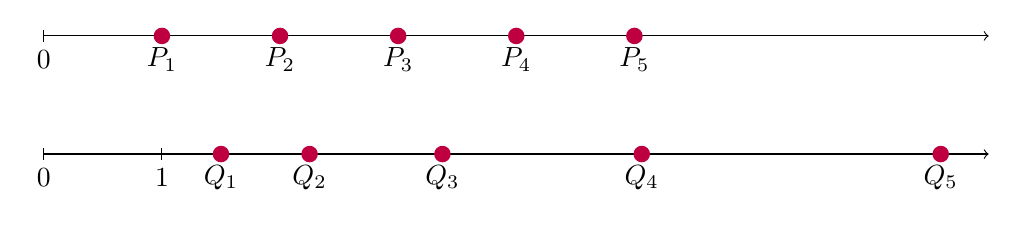
\begin{tikzpicture}[scale=1.5]
% \fill [white] (1.7,1.3) rectangle (6.25,2.3);
\draw [->](0,0)--(8,0);
\draw [->](0,-1)--(8,-1);
\draw (0,-0.05)--(0,0.05);
\node at (0,-0.2) {0};
\draw (0,-1.05)--(0,-0.95);
\node at (0,-1.2) {0};
\draw (1,-1.05)--(1,-0.95);
\node at (1,-1.2) {1};
\fill[purple,thick] (1,0) circle (0.7mm);
\node at (1,-0.2) {$P_1$};
\fill[purple,thick] (1.5,-1) circle (0.7mm);
\node at (1.5,-1.2) {$Q_1$};
\fill[purple,thick] (2,0) circle (0.7mm);
\node at (2,-0.2) {$P_2$};
\fill[purple,thick] (2.25,-1) circle (0.7mm);
\node at (2.25,-1.2) {$Q_2$};
\fill[purple,thick] (3,0) circle (0.7mm);
\node at (3,-0.2) {$P_3$};
\fill[purple,thick] (3.375,-1) circle (0.7mm);
\node at (3.375,-1.2) {$Q_3$};
\fill[purple,thick] (4,0) circle (0.7mm);
\node at (4,-0.2) {$P_4$};
\fill[purple,thick] (5.0625,-1) circle (0.7mm);
\node at (5.0625,-1.2) {$Q_4$};
\fill[purple,thick] (5,0) circle (0.7mm);
\node at (5,-0.2) {$P_5$};
\fill[purple,thick] (7.59375,-1) circle (0.7mm);
\node at (7.59375,-1.2) {$Q_5$};
\end{tikzpicture}
\end{center}

\captionof{figure}{Objetos movendo-se com velocidades distintas.}\label{Movimento}

Podemos, então, associar os pontos das duas semi-retas entendendo que dois pontos $P_t$ e $Q_t$ estão associados se os objetos $P$ e $Q$ estão nessas respectivas posições no mesmo instante $t$. Assim $Q_1$ está associado à 
$P_1$, $Q_2$ está associado à $P_2$ e assim por diante.

\begin{resposta}{Progressões}
{\begin{itemize}
\item $\{1,2,3,4,5,6,7,8,\cdots\};$
\item[] $\{2,4,8,16,32,64,\cdots\};$
\item $\{1,2,3,4,5,6,7,8,\cdots\};$
\item são os valores da primeira sequência.
\end{itemize}}
{1}
\end{resposta}

\begin{task}{Progressões}
Vamos pensar que o objeto $P$ na primeira reta move-se, a cada segundo, uma unidade para a direita e que inicia na origem. Já o objeto $Q$ inicia a duas unidades da origem e move-se, a cada segundo, uma quantidade de unidades igual à distância que está da origem. Escreva os 10 primeiros termos da sequência de distâncias à origem de cada um dos objetos.
\begin{itemize}
\item Você reconhece as duas sequências que estão se formando? 
\item Quais os valores dos logaritmos em base 2 dos valores encontrados na segunda sequência?
\item Você consegue reconhecer esses logaritmos na primeira sequência?
\end{itemize}
\end{task}

Observamos que a sequência das distâncias do ponto $Q$ à origem forma a P.G. $Q_n=r^n$, de razão $r$, e a sequências das distâncias do ponto $P$ à origem forma uma P.A. $P_n =n$. A interpretação de Napier é que o logaritmo do número $r^n$ da P.G. é o número associado na P.A., $n$. Assim, Napier associava os conceitos de P.A. e P.G. ao conceito de logaritmo.


\pagebreak


\know{A Lei de Weber.}

\begin{ObjetivoEsp}{A Lei de Weber.}
{Criar uma ferramenta para avaliar o custo benefício de um produto utilizando funções logarítmicas.}
{1}
\end{ObjetivoEsp}

\begin{Recomenda}{A Lei de Weber.}
{A seção "Para saber +: a lei de Weber"\, é opcional e propõem que o estudante crie uma escala para auxiliar em suas decisões financeiras. É a única atividade no material de logaritmos a estimular diretamente o desenvolvimento do nível mais alto da Taxonomia de Bloom Revisada - Criar.

Recomendamos que o/a professor/a desenvolva a atividade antes de trazê-la aos estudantes, para  melhor avaliar sua adequação à turma. Não apresentamos respostas para os exercícios, pois eles dependem das escolhas realizadas pelos estudantes.

Cabe ressaltar que não há respostas certas e que é possível que o estudante chegue a conclusão que a fórmula proposta (em toda a sua simplicidade e subjetividade) não auxilia no processo de escolha do produto com melhor relação de custo-benefício. Por fim incentiva-se que os estudantes reflitam sobre os resultados obtidos.}
{1}
\end{Recomenda}


Vamos considerar as seguintes situações:
\begin{enumerate}
\item Uma lanchonete vende um hambúrguer por R$\$$ 30,00 e outra lanchonete vende um hambúrguer similar por R$\$$ 20,00. A diferença de preço parece significativa para você? Seria importante na decisão de qual lanchonete visitar?
\item Uma loja de eletrodomésticos vende uma geladeira por R$\$$1.837,00 e outra loja vende uma geladeira similar por R$\$$1.847,00. A diferença de preço parece significativa para você? Seria importante na decisão de qual geladeira comprar?
\end{enumerate}

Muitas pessoas diriam que a diferença de R$\$$ 10,00 no primeiro caso é significativa, mas que a mesma diferença é irrelevante no segundo caso. Isso ocorre porque nossos sentidos percebem as mudanças de acordo com a magnitude dos valores envolvidos. Vimos exemplos de situações similares no Decibel, no pH e nas escalas Richter e de Magnitude de Momento Sísmico, nas quais são necessárias alterações significativas nos estímulos para percebermos diferença nos eventos.

A Lei de Weber, ou Lei de Weber-Fechner, foi proposta (para a percepção de pesos) por Ernst Heinrich Weber em 1834 e afirma que nossas percepções aos estímulos do mundo real variam de acordo com o tamanho dos estímulos e, deste modo, em escala logarítmica.

Essa lei empírica é utilizada para determinar alterações nos preços e nos tamanhos de embalagens de produtos (como o chocolate, por exemplo, cujas embalagens são frequentemente reduzidas).


\begin{resposta}{Criando a própria escala.}
{Apresentamos uma resposta como exemplo de desenvolvimento da atividade:
\begin{enumerate}
\item automóveis;
\item carro A 1.0 – R$\$ 40.000{,}00$ e carro B 1.3 – R$\$60.000{,}00$;
\item devido aos opcionais adicionados e o motor mais potente, considero o carro B 30$\%$ melhor;
\item $v(x) = 0{,}3\log_{3/2}\left(x/40000\right)$;
\item carro C 1.0 - R$\$ 48.000{,}00$, $p_c=10\%$; carro D 1.5 - R$\$ 65.000{,}00$, $p_d=35\%$; carro E 1.3 - R$\$ 50.000{,}00$, $p_e=25\%$;
\item $v(c) = 0{,}3\log_{3/2}\left(48/40\right) \approx 13{,}48\%$; $v(d) = 0{,}3\log_{3/2}\left(65/40\right) \approx 35{,}92\%$ e $v(e) = 0{,}3\log_{3/2}\left(45/40\right) \approx 16{,}51\%$;
\item $p_c = 10\% < 13{,}48\% = v(c)$, assim consideramos o carro $10\%$ melhor, mas seu valor relativo de compra é $13{,}48\%$ maior, desse modo seu custo relativo é maior do que o aumento no preço e sua aquisição não parece ser muito recomendável; $p_d = 35\% < 35{,}92\% = v(c)$, assim consideramos o carro é $35\%$ melhor e seu valor relativo de compra é $35{,}92\%$ maior, desse modo seu custo benefício é similar ao dos carros A e B; $p_e = 25\% > 16{,}51\% = v(e)$, assim consideramos o carro $25\%$ melhor, mas seu valor relativo de compra é $16{,}51\%$ maior, desse modo seu custo relativo é melhor do que os anteriores e sua aquisição parece mais recomendável;
\item a fórmula parece adequar os valores de modo a permitir comparar custo-benefício de produtos com preços bastante distintos. 
\end{enumerate}}
{1}
\end{resposta}


\begin{task}{Criando a própria escala.}
Vamos desenvolver a nossa própria escala para compararmos preços distintos? Isso precisará ser feito em etapas:
\begin{enumerate}
\item escolha uma categoria de produto, como automóveis, televisores, motocicletas, videogames, $\ldots$;
\item escolha dois produtos dentro da categoria, A e B, com preços $a$ e $b$, significativamente distintos, que tenham o mesmo custo-benefício para você;
\item determine um percentual $0 < p <1$, que o produto mais caro é melhor do que o produto mais barato para você (o que é subjetivo e não precisa estar diretamente ligado aos preços dos produtos);
\item escreva a sua própria função de valor relativo percentual através da expressão
$$
v(x)=p\log_{b/a} \left( \frac{x}{a} \right),
$$
de modo que $v(b) = p$ e $v(a)=a$, ou seja, $v(x)$ tenta estimar a diferença percentual no valor relativo do produto B com o produto A (para você);
\item encontre três produtos $C$, $D$ e $E$, na mesma categoria dos anteriores, anote os preços deles $c$, $d$ e $e$, e determine os percentuais $p_c$, $p_d$ e $p_e$ que eles são melhores ou piores do que o produto A (o que é subjetivo);
\item calcule $v(c)$, $v(d)$ e $v(e)$ e observe se os valores concordam com os percentuais que você estimou;
\item  $p_c, p_d, p_e$ são maiores, menores ou iguais a $v(c), v(d), v(e)$, respectivamente? o que essa informação diz sobre o custo benefício dos produtos?  
\item você acha que os resultados obtidos condizem com as suas percepções ou a fórmula apresentou grandes distorções?
\end{enumerate}
\end{task}

\pagebreak



%\clearmargin  %força comentários na próxima página
\begin{ObjetivoEsp}{Projeto Aplicado}
{Utilizar os conhecimentos sobre logaritmos como ferramenta para a tomada de decisão.}
{1}
\end{ObjetivoEsp}
\begin{Recomenda}{Projeto Aplicado}
{Essa atividade lúdica deve ser desenvolvida com toda a turma se for possível encaixá-la no cronograma da turma, pois está relacionada a habilidade EM13MAT203, que não precisa ser, necessariamente, trabalhada no contexto de logaritmos. A atividade ilustra como os logaritmos poderiam auxiliar na tomada de decisão em um contexto de matemática financeira. O professor precisará de papeletes ou um dado de 10 faces para realizar os sorteios.

No item a), o professor pode discutir com os estudantes os cálculos que devem ser realizados, e apresentar os valores dos logaritmos.

No item b) o/a professor/a deve sortear números mensalmente e os alunos vão saindo da brincadeira conforme seus números são sorteados, até que alguém atinja o objetivo.

Obs: quem escolheu o plano A não vai  sair, mas como sua taxa de juros é baixa, até que ele atinja o valor, outro aluno pode vencer antes, daí ele também perde. Se todos os outros perderem os investidores do plano A são os vencedores. }
{1}
\end{Recomenda}
\begin{resposta}{Projeto aplicado} 
{\begin{itemize}
\item[] Plano A - $\log_{1,01} 1,5 \approx 40,75$, portanto serão necessários 41 meses; 
\item[] Plano B - $\log_{1,02} 1,5 \approx 20,48$, portanto serão necessários 21 meses;
\item[] Plano C - $\log_{1,05} 1,5 \approx 8,31$, portanto serão necessários 9 meses;
\item[] Plano D - $\log_{1,07} 1,5 \approx 5,99$, portanto serão necessários 6 meses.
\end{itemize}}
{1}
\end{resposta}\begin{project}
Um banco tem 4 opções de investimento (A : sem risco, B: baixo risco, C: médio risco e D: alto risco), com taxas de juros mensais de $1\%$, $2\%$, $5\%$ e $7\%$ respectivamente. Você investirá R$\$ 10.000,00$ em um desses investimentos e quer obter R$\$15.000,00$.

\begin{enumerate}
\item Quantos meses você levará para atingir seu objetivo em cada um dos Planos?

\begin{table}[H]
\centering
\begin{tabular}{|l|l|l|l|l|}
\hline
\rowcolor[HTML]{00A59D} 
\cellcolor[HTML]{EFEFEF}Plano & A   & B   & C   & D   \\ \hline
\rowcolor[HTML]{FFFFFF} 
\cellcolor[HTML]{EFEFEF}Taxa  & 1\% & 2\% & 5\% & 7\% \\ \hline
\rowcolor[HTML]{FFFFFF} 
\cellcolor[HTML]{EFEFEF}Tempo &  \hspace{25mm}   &  \hspace{25mm}   &  \hspace{25mm}   &  \hspace{25mm}   \\ \hline
\end{tabular}
\end{table}

\item Nesse item propomos um jogo. “JOGO DE RISCO” depois que os alunos calcularem o tempo (em meses) para acumular o valor desejado eles devem escolher um dos planos possíveis para investir seu capital. Cada aluno escolhe, então, 0, 1, 2 ou 3 “números do azar” de 0 a 9. Quem escolheu o plano A escolhe 0 números de azar e quem escolheu D deve escolher 3 números. A cada mês o professor sorteará um número de 0 a 9 e aqueles que tiverem o número sorteado perdem tudo e saem do jogo. O primeiro a atingir o montante desejado vence.
\end{enumerate}
\end{project}


\pagebreak

\ifnum \aluno=1
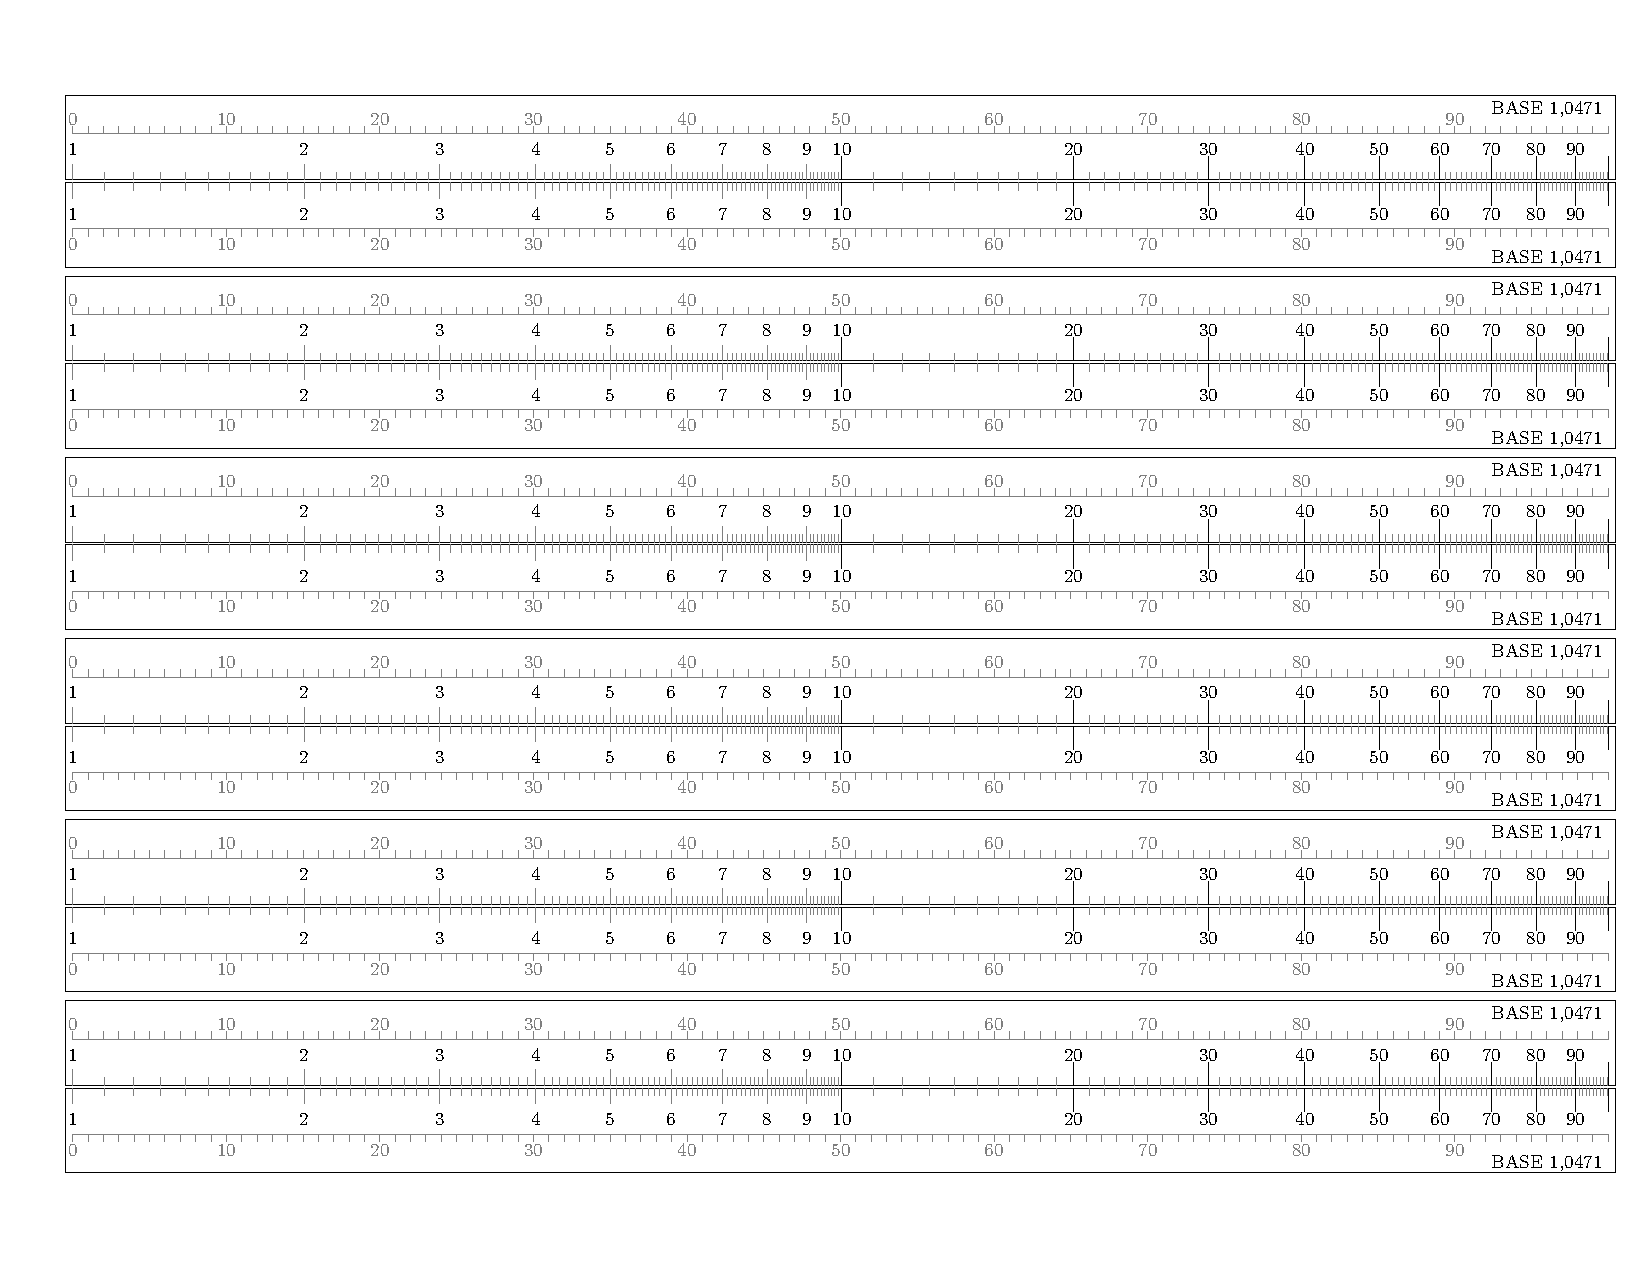
\includepdf[angle=-90]{Figuras/Ruler.pdf}
\else
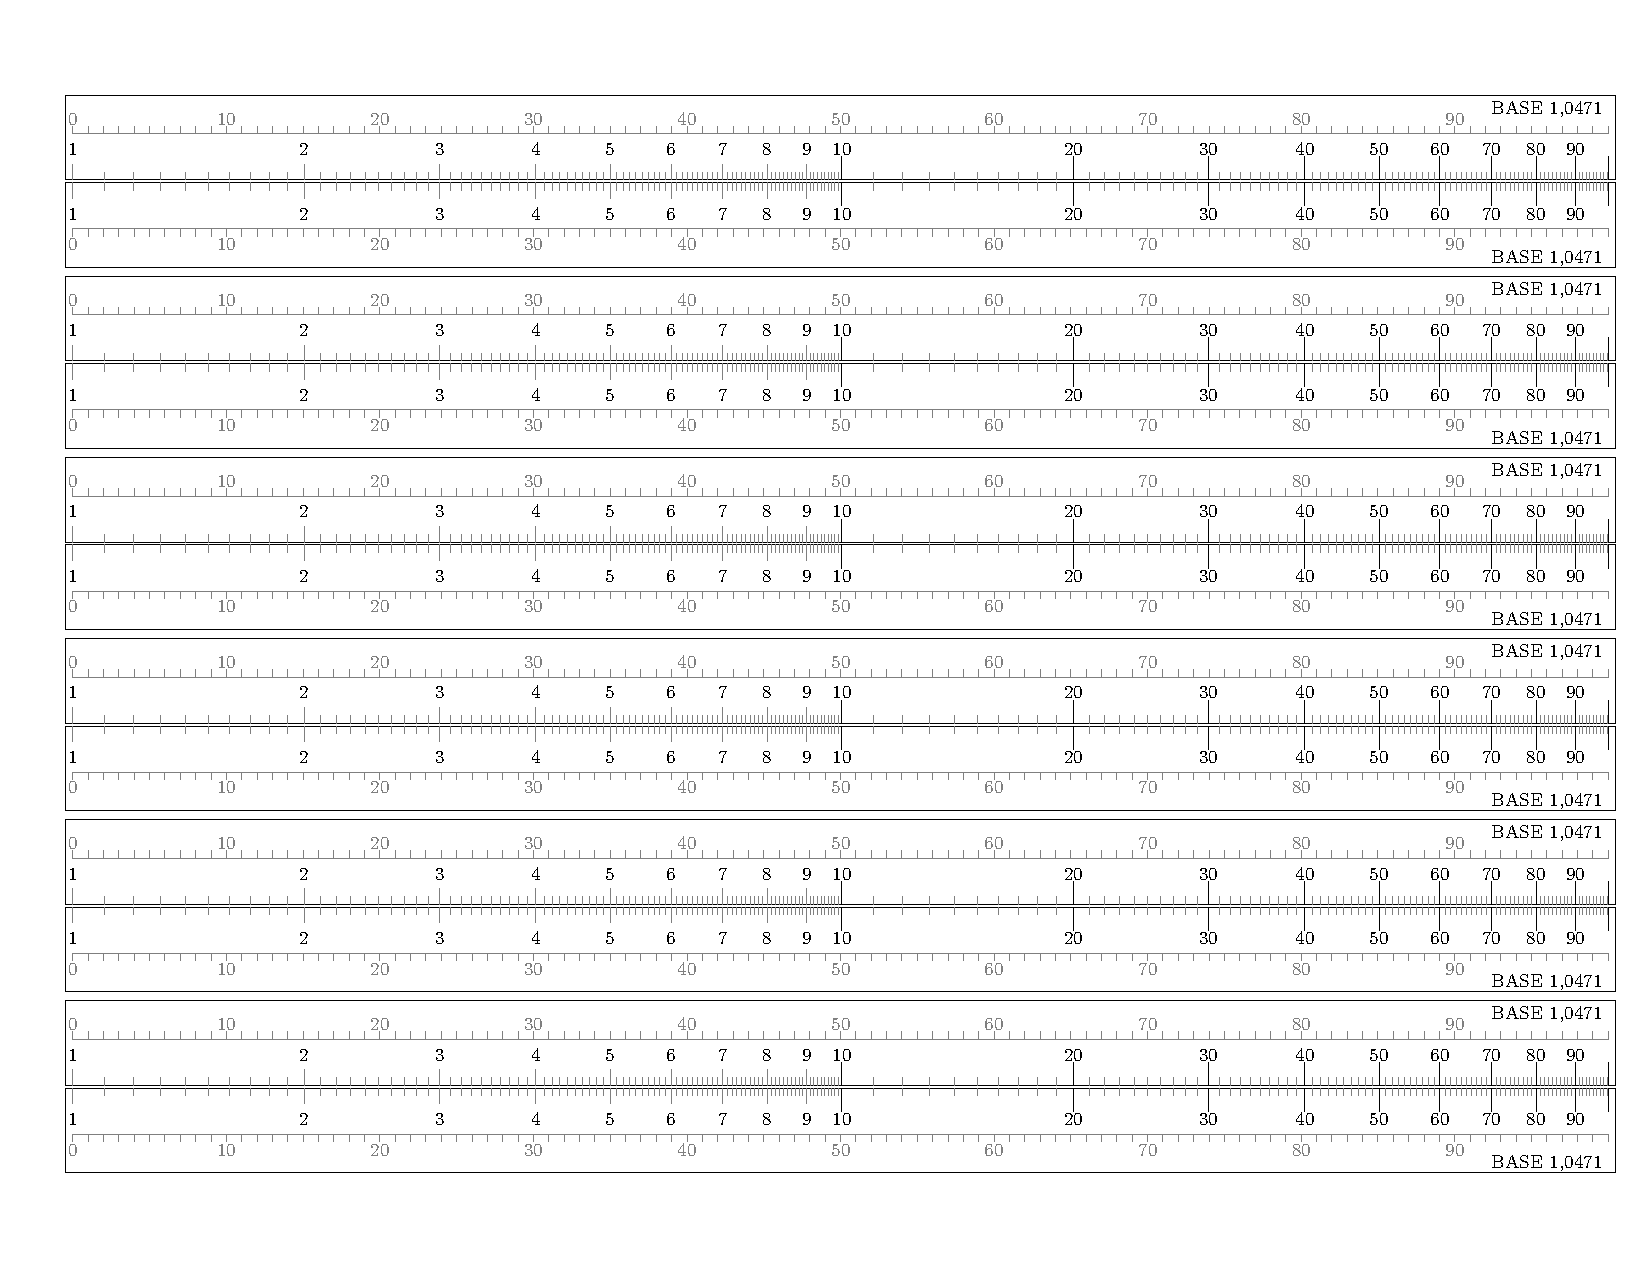
\includepdf[angle=-90, offset = 0mm 2mm]{Figuras/Ruler.pdf}
\fi



%
%
